\chapter{Implementasi dan Pengujian}
\label{chap:implementasiPengujian}

Bab ini terdiri atas dua bagian, yaitu Implementasi Perangkat Lunak dan Pengujian Perangkat Lunak. Bagian implementasi berisi penjelasan lingkungkan pengembangan perangkat lunak dan hasil implementasi. Sedangkan bagian pengujian berisi hasil pengujian fungsional dan eksperimental terhadap perangkat lunak yang telah dibangun.

\section{Implementasi}
\label{sec:implementasi}

\subsection{Lingkungan Implementasi}
		\label{sec:lingkungan_implementasi}
			Lingkungan implementasi yang digunakan adalah Heroku \footnote{\url{https://devcenter.heroku.com/categories/reference}}. Heroku merupakan \textit{cloud platform} yang menyediakan fitur yang dapat membantu pengguna untuk dapat memiliki alamat domain. Semua aplikasi Heroku dijalankan dalam koleksi kontainer Linux ringan yang disebut dynos. Spesifikasi Heroku yang digunakan oleh IFStudentPortal akan dijelaskan pada Tabel \ref{tab:dynotype}
\begin{table}[H]
	\centering
		\caption{Spesifikasi Heroku}
			\begin{tabular}{ |p{2.65cm}|p{1.5cm}|p{2cm}|p{1.5cm}|p{1.5cm}|p{1.5cm}|p{1.5cm}|}
			\hline
			Dyno Type & Sleeps & Professional Features & Memory (RAM) & CPU Share & Dedicated & Compute \\ \hline
			free & yes & no & 512 MB & 1x & no & 1x-4x \\ \hline
			hobby & no & no & 512 MB & 1x & no & 1x-4x \\ \hline
			standard-1x & no & yes & 512 MB & 1x & no & 1x-4x \\ \hline
			standard-2x & no & yes & 1024 MB & 2x & no & 4x-8x \\ \hline
			performance-m & no & yes & 2.5 GB & 100\% & yes & 11x \\ \hline
			performance-l & no & yes & 15 GB & 100\% & yes & 46x \\ \hline
			\end{tabular}
		\label{tab:dynotype}
\end{table}
			Dari tabel \ref{tab:dynotype} penjelasan detail dari masing-masing kolom adalah sebagai berikut:
			\begin{enumerate}
				\item \textbf{Dyno Type}, Heroku menyediakan sejumlah \textit{dyno type} yang berbeda masing-masing dengan satu set properti unik dan karakteristik kinerja.
				\item \textbf{Sleeps}, jika aplikasi memiliki \textit{web dyno}, dan \textit{web dyno} tidak menerima \textit{traffic} dalam periode 30 menit, \textit{web dyno} akan tidur. Selain \textit{web dyno} yang sedang tidur, \textit{worker dyno} (jika ada) juga akan tidur. Jika \textit{web dyno} tidur menerima \textit{web traffic}, maka akan menjadi aktif kembali setelah penundaan singkat. Jika aplikasi memiliki \textit{worker dyno} yang ditingkatkan sebelum tidur, maka akan ditingkatkan lagi juga.  
				\item \textbf{Professional Features}, \textit{dyno type} yang digunakan adalah \textit{free}, sehingga fitur profesional seperti \textit{horizontal scalability, application metrics, dan preboot} tidak ada pada \textit{dyno type} tersebut.
				\item \textbf{Memory (RAM)}, RAM yang digunakan adalah sebesar 512 MB.
				\item \textbf{CPU Share}, menentukan alokasi daya pemrosesan yang dialokasikan ke \textit{Virtual Machine} dalam layanan \textit{Cloud}.
				\item \textbf{Compute}, Heroku \textit{compute unit} hanya \textit{Amazon compute unit} (karena Heroku berjalan diatas AWS). Satu unit komputasi pada AWS didefinisikan sebagai kekuatan komputer dari 1.0-1.2Ghz dari \textit{CPU server 2007}.
			\end{enumerate}
			
\subsection{Implementasi IFStudentPortal ke Heroku}
Langkah-Langkah implementasi IFStudentPortal ke Heroku, yaitu:
\begin{enumerate}
	\item Membuat akun heroku yang dapat dibuat pada alamat situs berikut \url{https://signup.heroku.com/}.
	\item Setelah membuat akun heroku kemudian \textit{login} dengan akun yang sudah dibuat.
	\item Setelah login akan diarahkan ke halaman \textit{dashboard} dari heroku, kemudian pilih ``create new app''.
	\item Kemudian masukkan nama aplikasi ``ifstudentportalskripsi'' dan klik ``create app''.
	\item Setelah berhasil, masuk ke menu ``deploy'' disana terdapat beberapa cara untuk melakukan \textit{deploy} ke heroku.
	\item Metode yang digunakan untuk deploy IFStudentPortal ke Heroku yaitu menggunakan ``heroku git'', beberapa langkah sebelum melakukan deploy, yaitu
	\begin{enumerate}
		\item Melakukan \textit{git clone } \url{https://github.com/AndriantoSugiarto/IFStudentPortal.git} pada ``terminal'' atau ``command prompt'' dari sistem operasi yang digunakan.
		\item Mengubah secret key pada file ``conf/application.conf'' dan mengikuti petunjuk cara mengubah secret key pada playframework di \url{https://www.playframework.com/documentation/2.6.x/ApplicationSecret}.
		\item Mengunduh dan menginstall ``Heroku CLI''
		\item Setelah berhasil menginstall ``Heroku CLI'', kemudin melakukan perintah ``heroku login''.
		\item Kemudian melakukan perintah ``heroku git:remote -a ifstudentportalskripsi''.
		\item Kemudian melakukan perintah ``git push heroku master'' untuk melakukan \textit{deploy} IFStudentPortal ke heroku.
		\item Setelah berhasil melakukan \textit{deploy} aplikasi dapat diakses melalui alamat ``\url{http://ifstudentportalskripsi.herokuapp.com/}''.
	\end{enumerate}
\end{enumerate}
\subsection{Hasil Implementasi}
		Hasil implementasi berupa aplikasi berbasis web yang dikembangkan untuk menyesuaikan dengan StudentPortal versi 2018 dan Kurikulum 2018. Aplikasi dapat diakses dengan URL \url{https://ifstudentportalskripsi.herokuapp.com}. Aplikasi Informatika Student Portal terdiri dari lima halaman antara lain:
		\begin{enumerate}
			\item\textbf{Halaman \textit{Login}}\\
				Halaman \textit{login} digunakan pengguna untuk masuk ke dalam aplikasi. Pada halaman ini, pengguna dapat melakukan \textit{login} dengan mengisi \textit{email} pada kolom \textit{email} dan \textit{password} pada kolom \textit{password} kemudian mengklik tombol login. Tangkapan layar dari halaman \textit{login} dapat dilihat pada Gambar \ref{fig:5_halaman_login}.
					\begin{figure}[H]
						\centering
						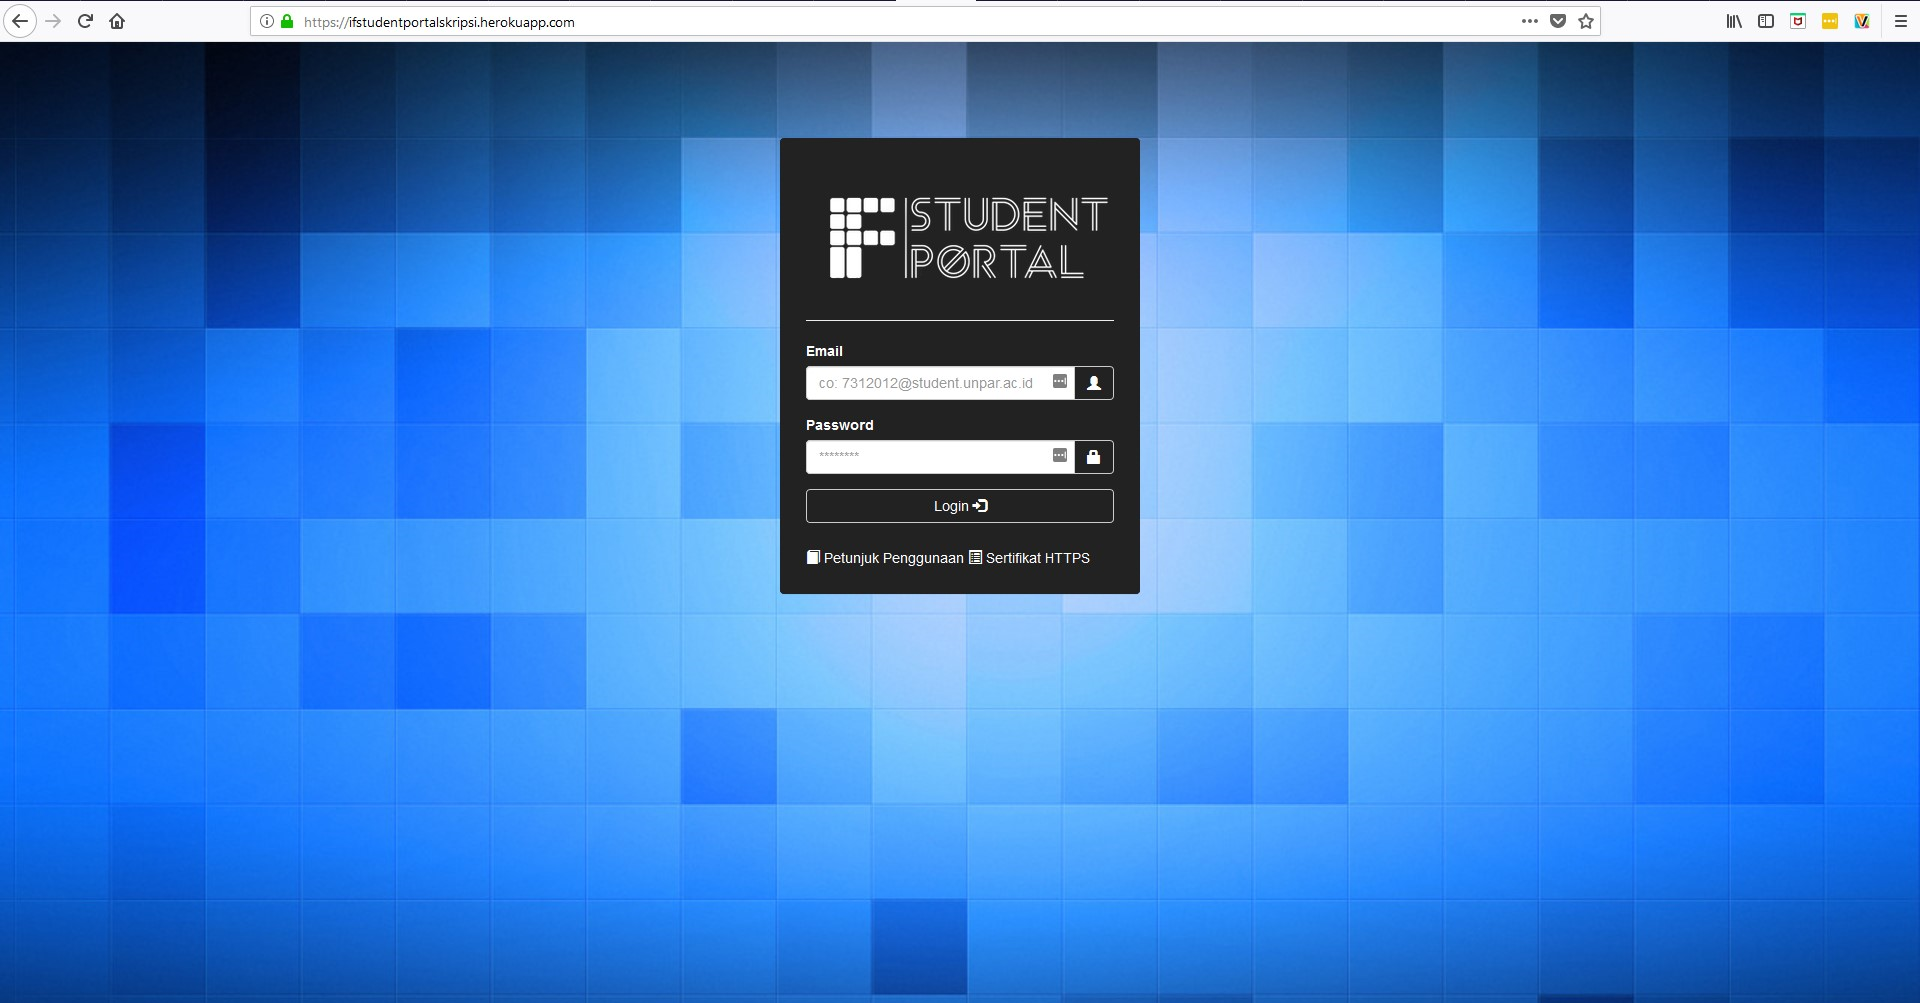
\includegraphics[scale=0.34]{Gambar/halaman_login}
						\caption{Halaman \textit{Login}} 
						\label{fig:5_halaman_login}
					\end{figure}
					
				\item\textbf{Halaman \textit{Home}}\\
				Halaman utama merupakan halaman yang pertama kali dituju setelah melakukan \textit{login}. Halaman utama menampilkan identitas pengguna dan \textit{link} menuju kode sumber aplikasi Informatika Student Portal. Tangkapan layar dari halaman utama dapat dilihat pada Gambar \ref{fig:5_halaman_utama}.
					\begin{figure}[H]
						\centering
						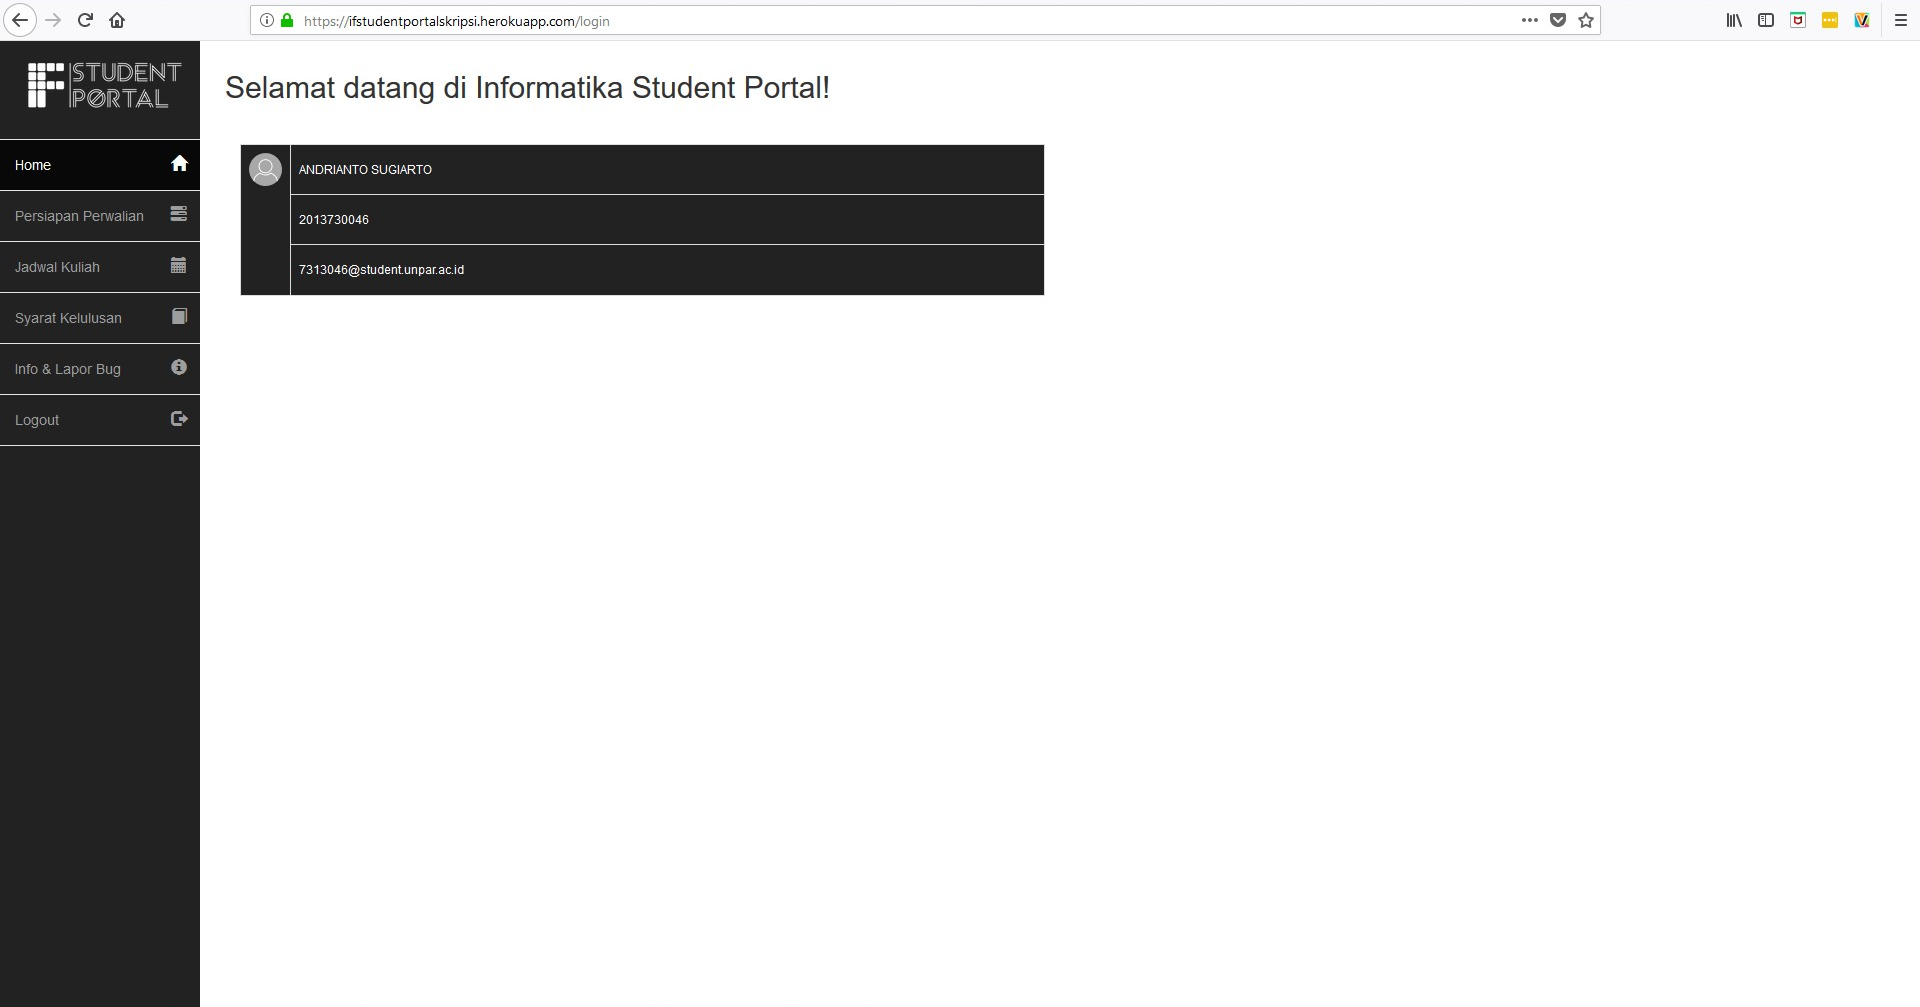
\includegraphics[scale=0.34]{Gambar/halaman_home}
						\caption{Halaman \textit{Home}} 
						\label{fig:5_halaman_utama}
					\end{figure}
						
				\item\textbf{Halaman Persiapan Perwalian}\\
				Halaman ini menampilkan data akademik dan tabel prasyarat mata kuliah. Pengguna dapat mengklik kode mata kuliah, kemudian akan diarahkan ke kode sumber aturan prasyarat mata kuliah tersebut. Tangkapan layar dari halaman prasyarat mata kuliah dapat dilihat pada Gambar \ref{fig:5_halaman_persiapan_perwalian}.
					\begin{figure}[H]
						\centering
						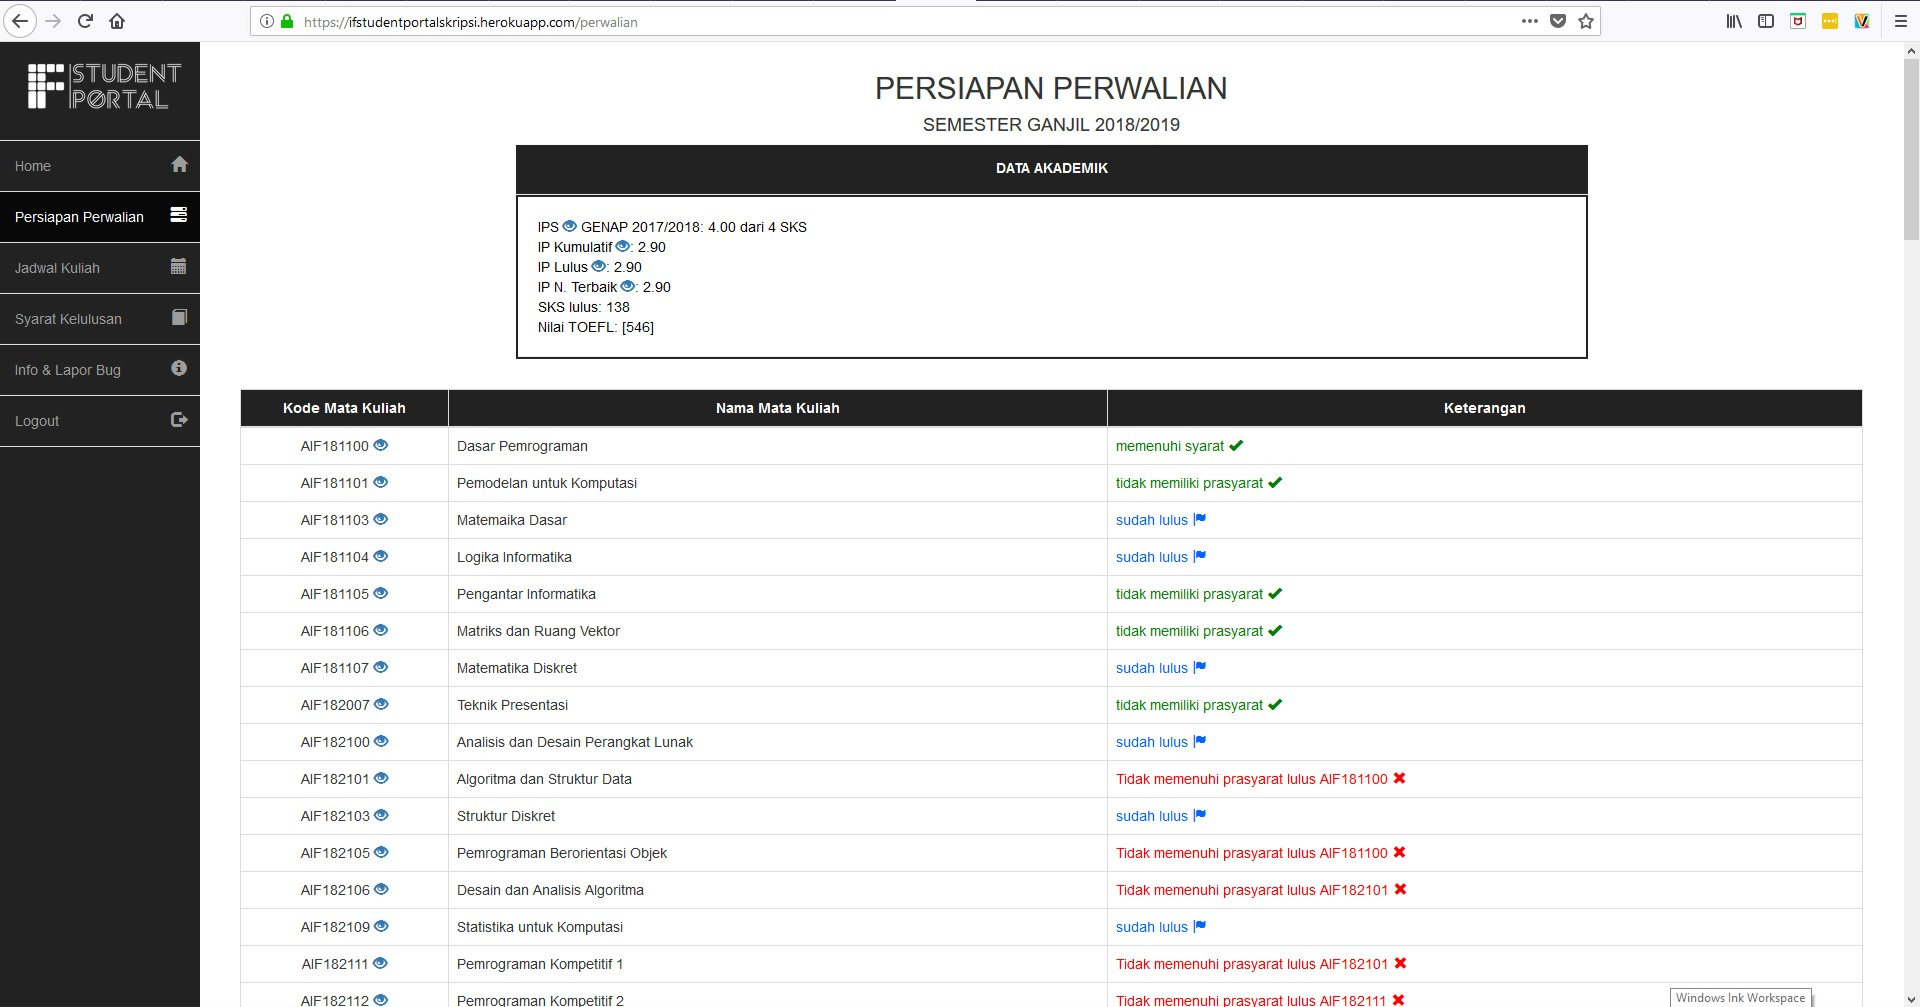
\includegraphics[scale=0.34]{Gambar/halaman_persiapan_perwalian}
						\caption{Halaman Persiapan Perwalian} 
						\label{fig:5_halaman_persiapan_perwalian}
					\end{figure}

				\item\textbf{Halaman Jadwal Kuliah}\\
				Halaman ini menampilkan jadwal kuliah yang tersusun dan terurut berdasarkan hari. Tangkapan layar dari halaman jadwal kuliah dapat dilihat pada Gambar \ref{fig:5_halaman_jadwal}. Jika kode mata kuliah diklik, akan muncul \textit{popup} seperti pada Gambar \ref{fig:5_halaman_jadwal_rinci} yang berisi rincian dari jadwal kuliah tersebut.
				\begin{figure}[H]
						\centering
						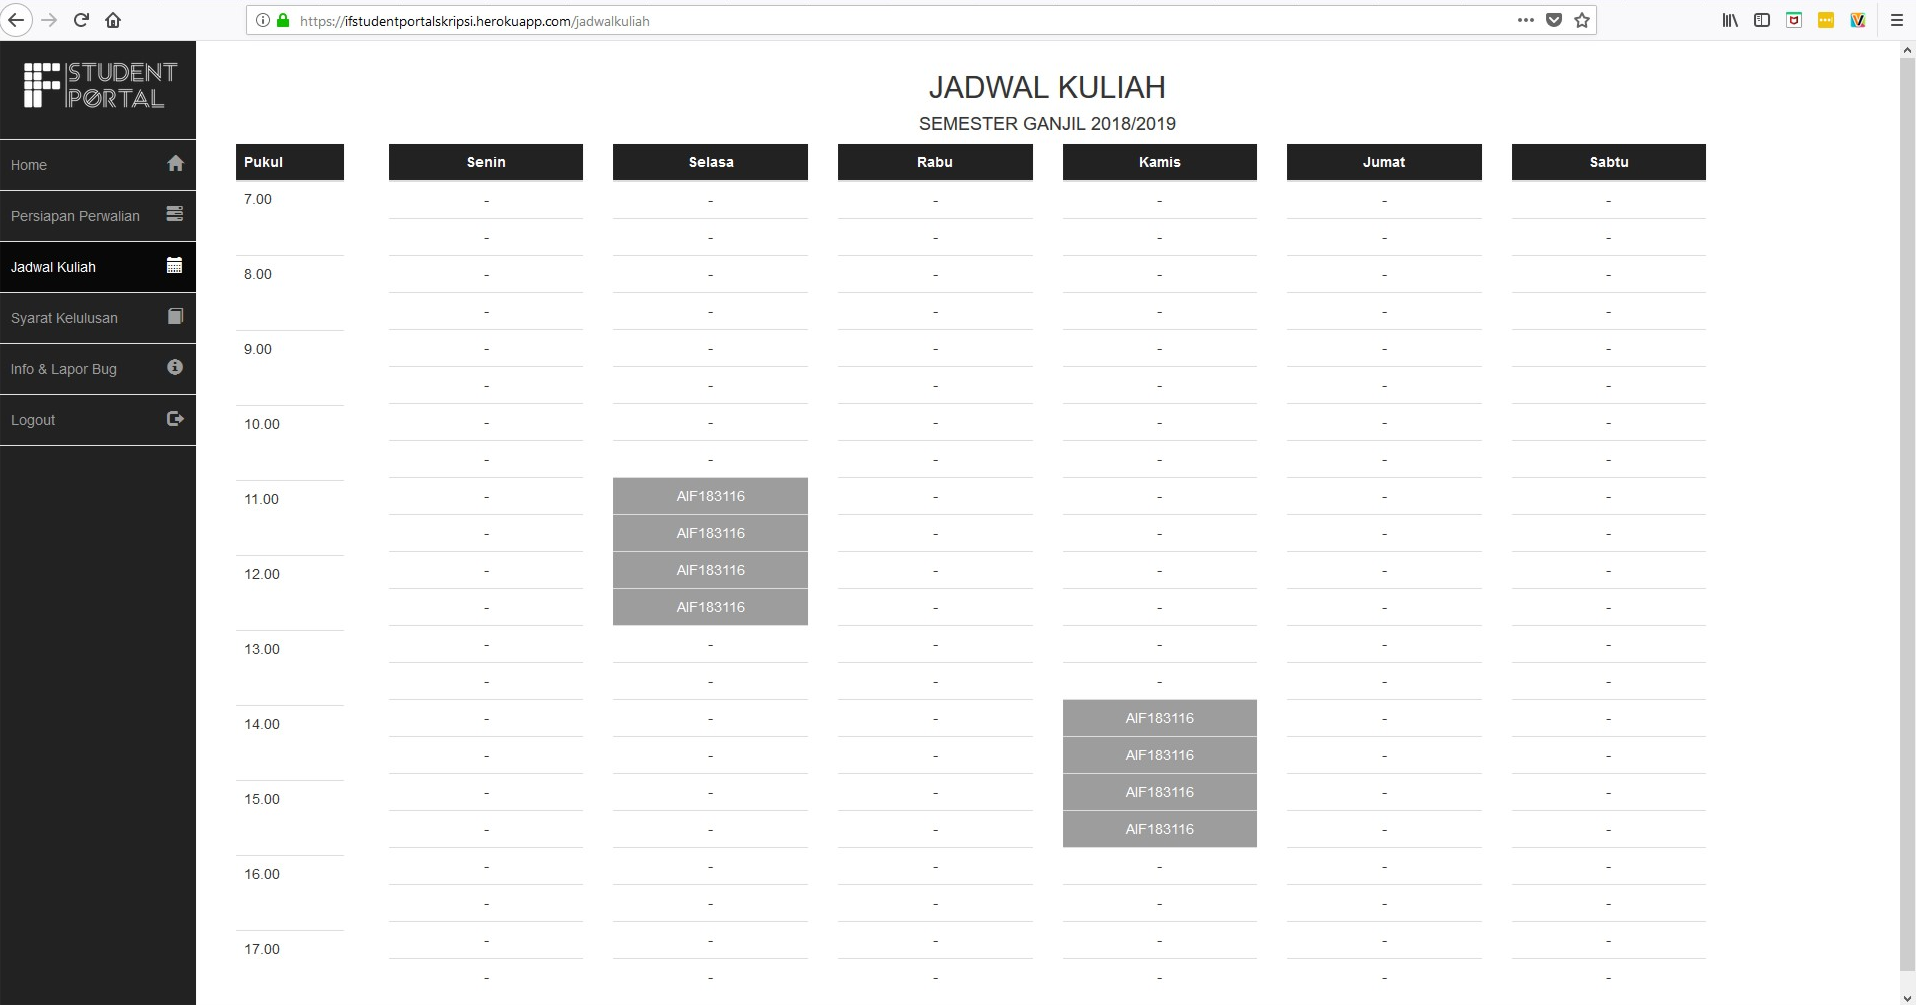
\includegraphics[scale=0.34]{Gambar/halaman_jadwal}
						\caption{Halaman Jadwal Kuliah} 
						\label{fig:5_halaman_jadwal}
					\end{figure}
					
					\begin{figure}[H]
						\centering
						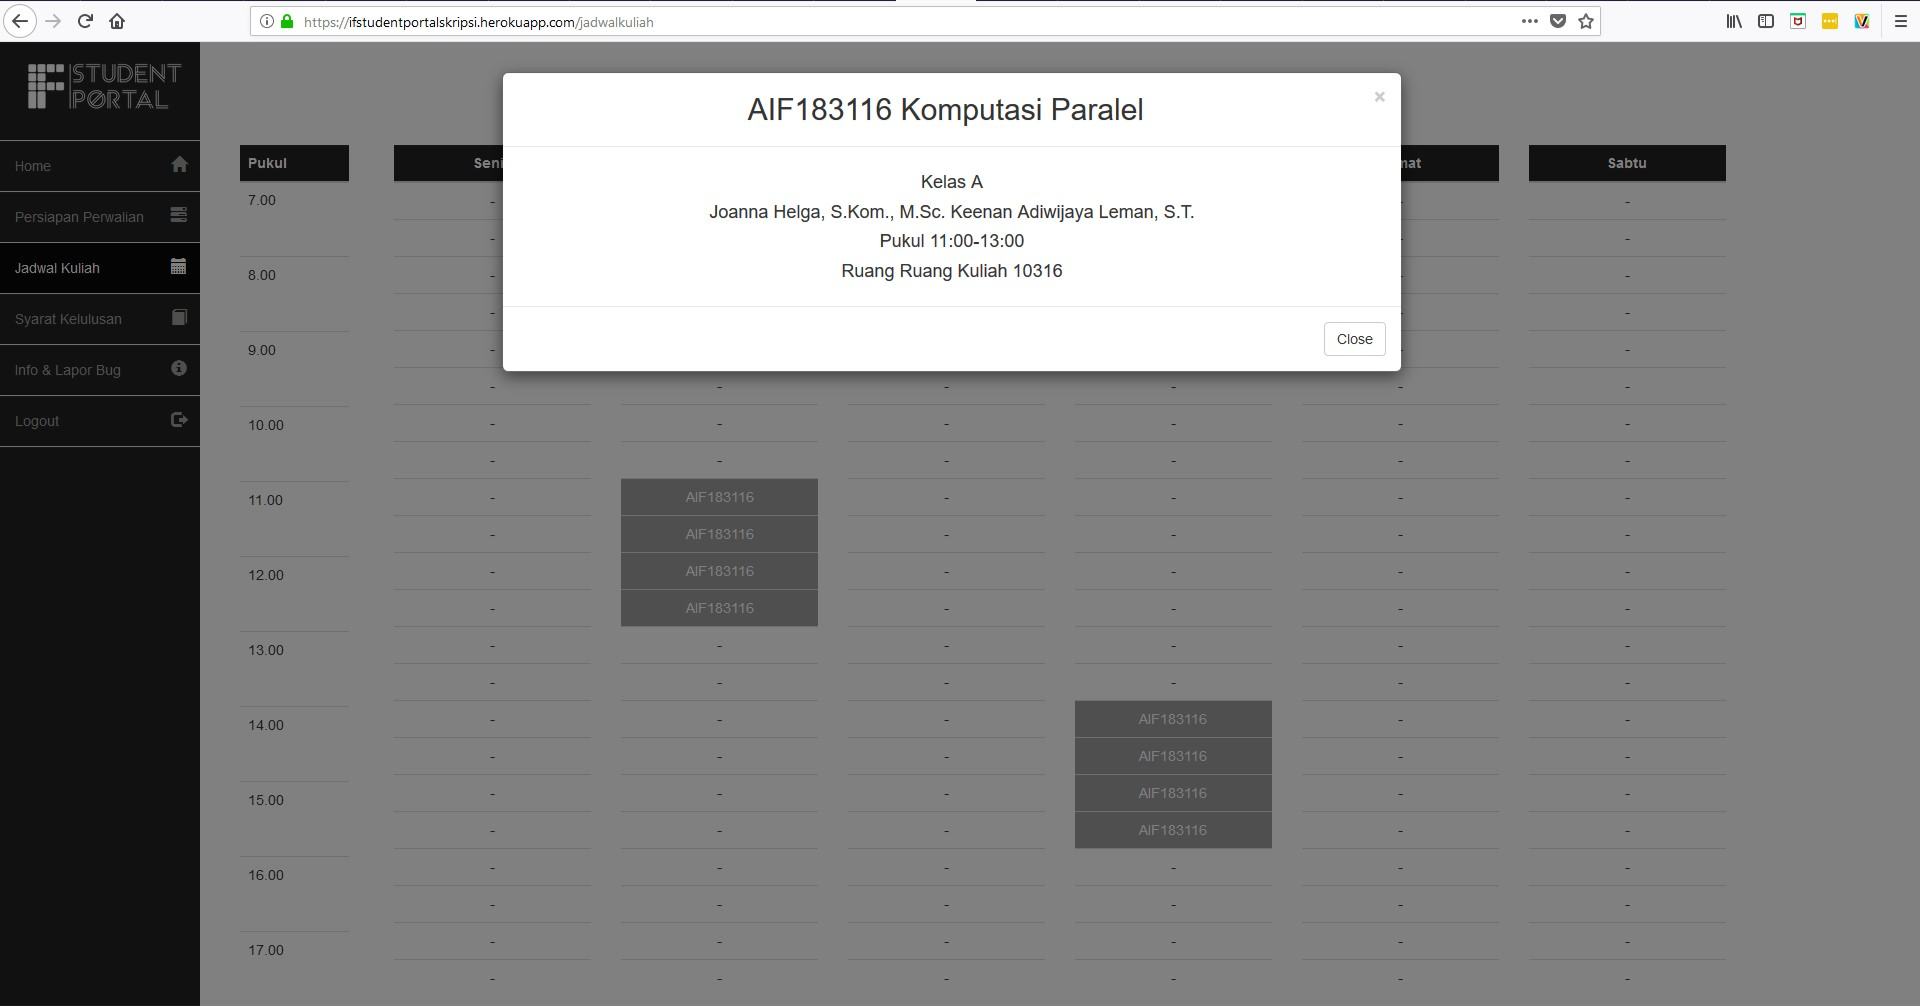
\includegraphics[scale=0.34]{Gambar/halaman_jadwal_rinci}
						\caption{Rincian Jadwal Kuliah} 
						\label{fig:5_halaman_jadwal_rinci}
					\end{figure}
					
				\item\textbf{Halaman Syarat Kelulusan}\\
				Halaman ini menampilkan syarat kelulusan dari Program Studi Teknik Informatika yang belum dipenuhi oleh mahasiswa. Tangkapan layar dari halaman data akademik dapat dilihat pada Gambar \ref{fig:5_halaman_syarat_kelulusan}.
				\begin{figure}[H]
						\centering
						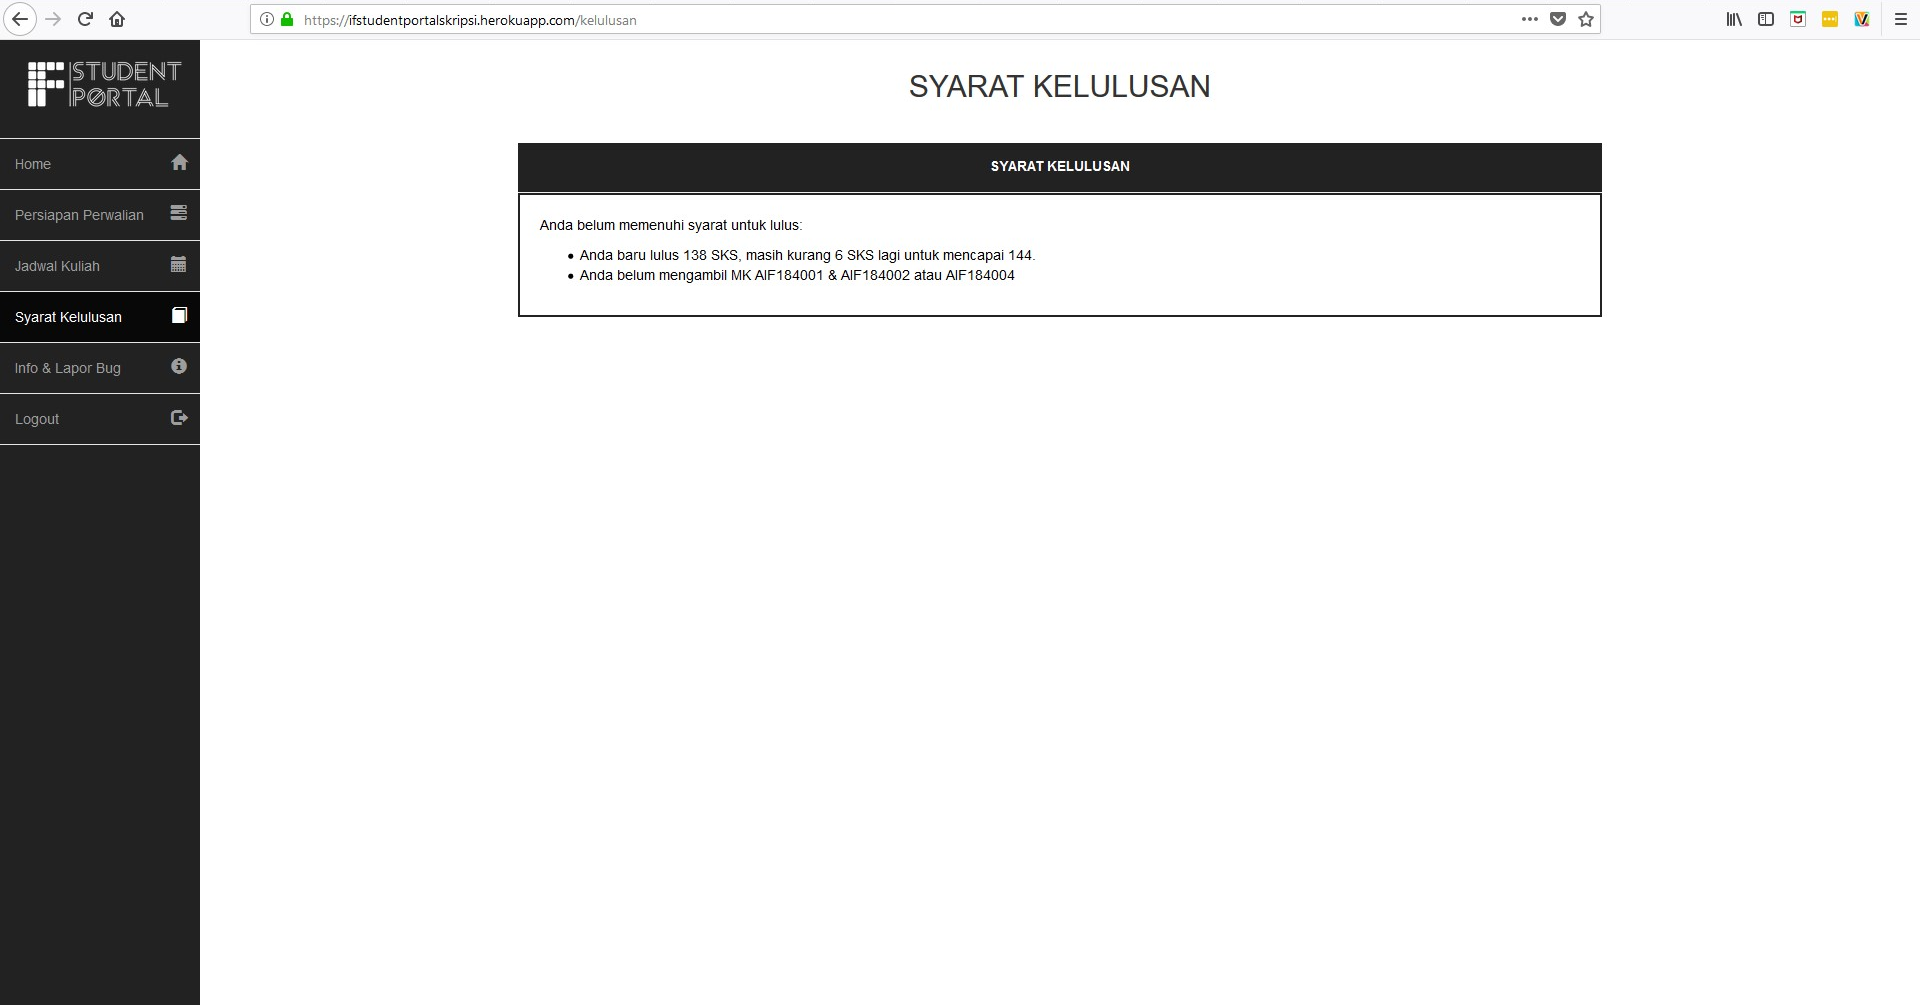
\includegraphics[scale=0.34]{Gambar/halaman_syarat_kelulusan}
						\caption{Halaman Syarat Kelulusan} 
						\label{fig:5_halaman_syarat_kelulusan}
					\end{figure}
		\end{enumerate}
		
\section{Pengujian}

\subsection{Pengujian Fungsional}
\label{subsec:fungsional}

Pengujian fungsional dilakukan sekitar bulan oktober sampai november untuk mengetahui kesesuaian reaksi perangkat lunak dengan reaksi yang diharapkan berdasarkan aksi pengguna terhadap perangkat lunak. Pengujian dilakukan pada \textit{cloud platform} dan Windows dengan hasil yang sama.

			\begin{table}[H]
			\centering
			\caption{Tabel Pengujian Fungsional}
				\begin{tabular}{|p{0.25cm}| p{3.5cm}| p{7cm}| p{2.5cm}|} \hline
				No.	&	Aksi Pengguna	&	Reaksi yang diharapkan	&	Reaksi Perangkat Lunak \\ \hline
				1.	&	Pengguna menjalankan aplikasi	&	Halaman \textit{login} akan ditampilkan	&	sesuai	\\ \hline
				2.	&	Pengguna memasukkan \textit{email} dan \textit{password}	&	Jika \textit{email} dan \textit{password}	sesuai, pengguna akan diarahkan ke halaman utama. & sesuai\\ \hline
				3.	&	Pengguna memilih menu ``Perwalian'' &	Jika pengguna belum memiliki riwayat nilai(masih menempuh semester 1), akan ditampilkan pesan ``DATA AKADEMIK BELUM TERSEDIA'' dan ``PRASYARAT BELUM TERSEDIA''	&	sesuai	\\ \hline
					&	&	Jika pengguna sudah memiliki riwayat nilai	akan ditampilkan tabel prasyarat mata kuliah beserta status pengambilannya dan ringkasan data akademik mahasiswa berupa IPS semester terakhir, IPK, IP Lulus, IP N. Terbaik, SKS Lulus, dan nilai TOEFL &	sesuai	\\ \hline
				4.	&	Pengguna memilih menu ``Jadwal Kuliah'' &	Jika pengguna belum melakukan FRS, cuti studi, atau jadwal kuliah pengguna belum tersedia, akan ditampilkan pesan ``JADWAL KULIAH BELUM TERSEDIA''	&	sesuai	\\ \hline
					&	&	Jika jadwal kuliah pengguna sudah tersedia, akan ditampilkan jadwal kuliah dalam bentuk kalendar yang sudah diurutkan berdasarkan hari &	sesuai	\\ \hline
				5.	&	Pengguna memilih menu ``Syarat Kelulusan'' &	Jika pengguna belum memiliki riwayat nilai(masih menempuh semester 1), akan ditampilkan pesan ``DATA AKADEMIK BELUM TERSEDIA'' &	sesuai	\\ \hline
					&	&	Jika pengguna sudah memiliki riwayat nilai, akan ditampilkan syarat kelulusan yang belum dipenuhi dari mahasiswa &	sesuai	\\ \hline
				6.	&	Pengguna memilih tombol \textit{logout}	&	Pengguna akan diarahkan kembali ke halaman \textit{login} &	sesuai	\\ \hline
				7.	& Dua pengguna menggunakan aplikasi secara bersamaan	&	Pengguna dapat menggunakan aplikasi dengan akun yang sesuai &	sesuai	\\ \hline
				\end{tabular}
				\label{table:hasilFungsional}
			\end{table}
			
\subsection{Pengujian Eksperimental}
Pengujian eksperimental dilakukan terhadap mahasiswa Teknik Informatika UNPAR angkatan 2013 sampai 2018 dan Mahasiswa Teknik informatika UNPAR yang sudah lulus. Dari setiap angkatan, diambil dua orang untuk melakukan pengujian. Setiap responden diminta untuk melakukan \textit{login} kemudian melihat dari setiap halaman pada Student Portal dan memastikan apakah data tersebut sesuai dengan data sebenarnya. Pengujian eksperimental sempat terjadi masalah, karena saat pengujian ekspermintal dilakukan sekitar awal bulan november nilai per semester pada StudentPortal menjadi kosong. Tanggal 14 November nilai per semester telah muncul kembali, sehingga pengujian eksperimental kembali dilakukan.
Hasil pengujian eksperimental dirangkum sebagai berikut:
\begin{itemize}
	\item Angkatan 2013 \\
	Untuk angkatan 2013 pengujian dilakukan kepada dua orang mahasiswa, yaitu:
	\begin{enumerate}
		\item Steven Haryanto - 2013730028 \\
		\begin{figure}[H]
			\centering
			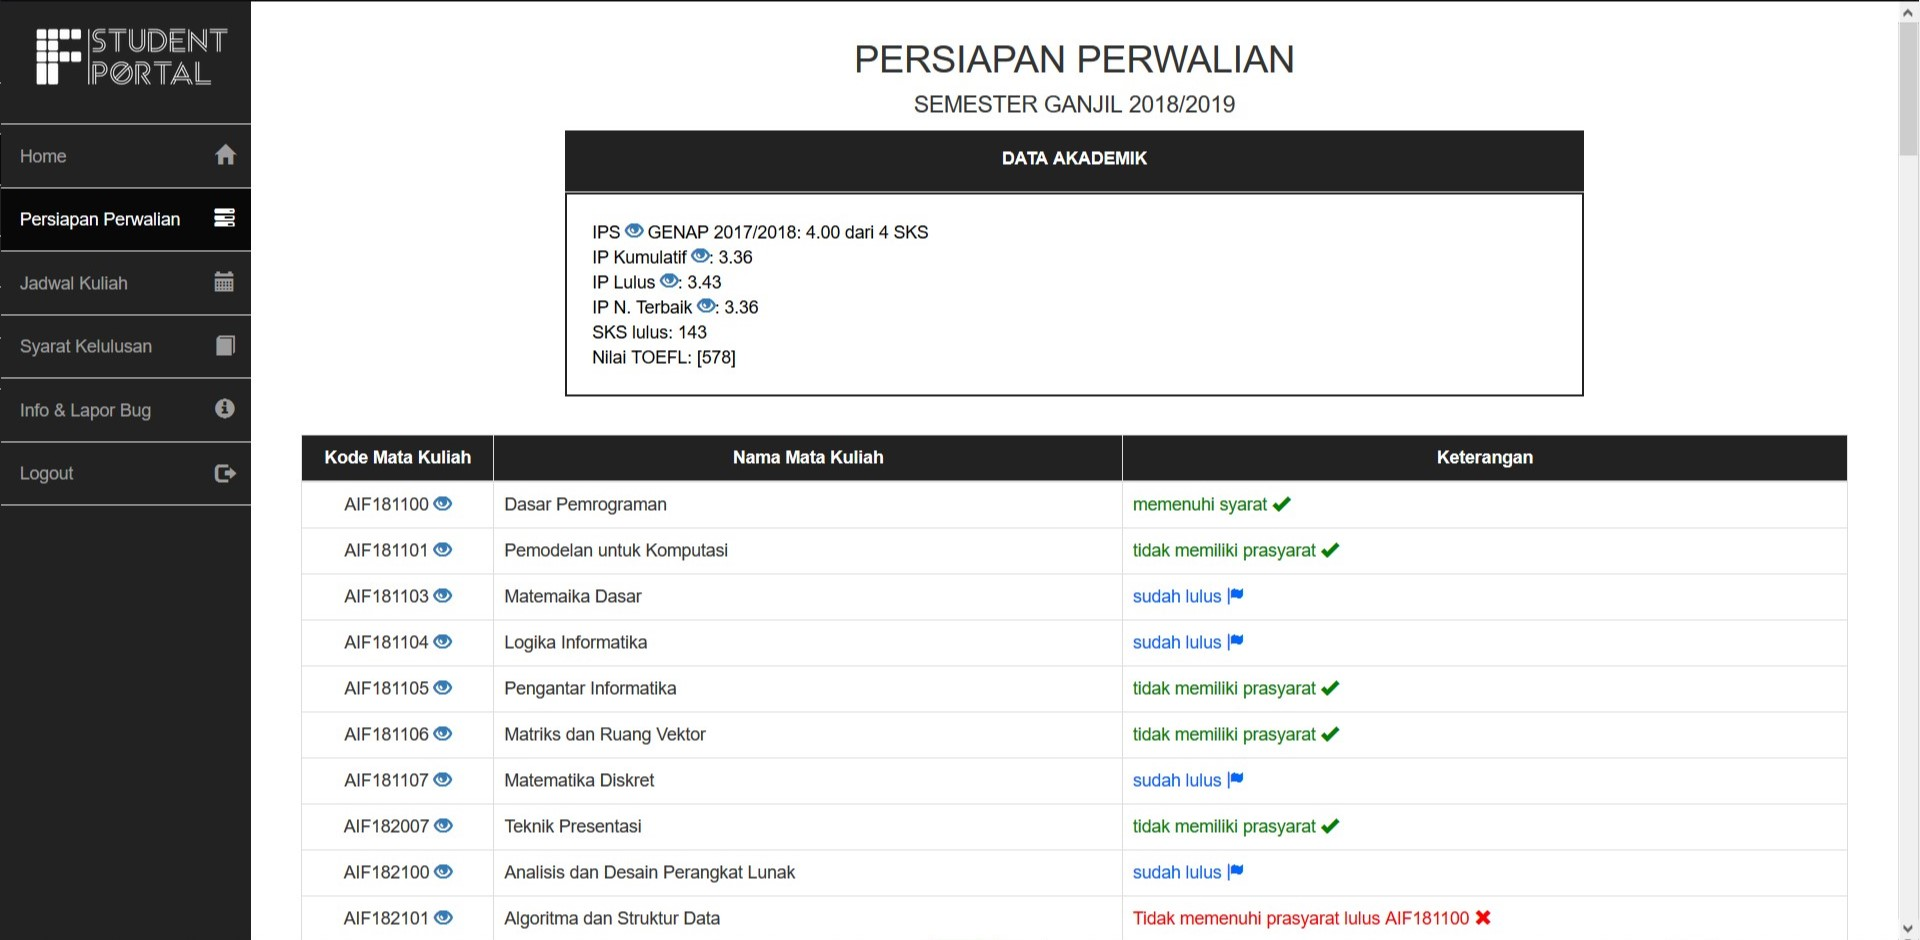
\includegraphics[scale=0.425]{Gambar/HasilPengujian/2013_1_persiapan_perwalian_ifstudentportal}
			\caption{Halaman Persiapan Perwalian (IFStudentPortal) - Steven Haryanto}
			\label{fig:2013_1_persiapan_perwalian_ifstudentportal}
		\end{figure}
		\begin{figure}[H]
			\centering
			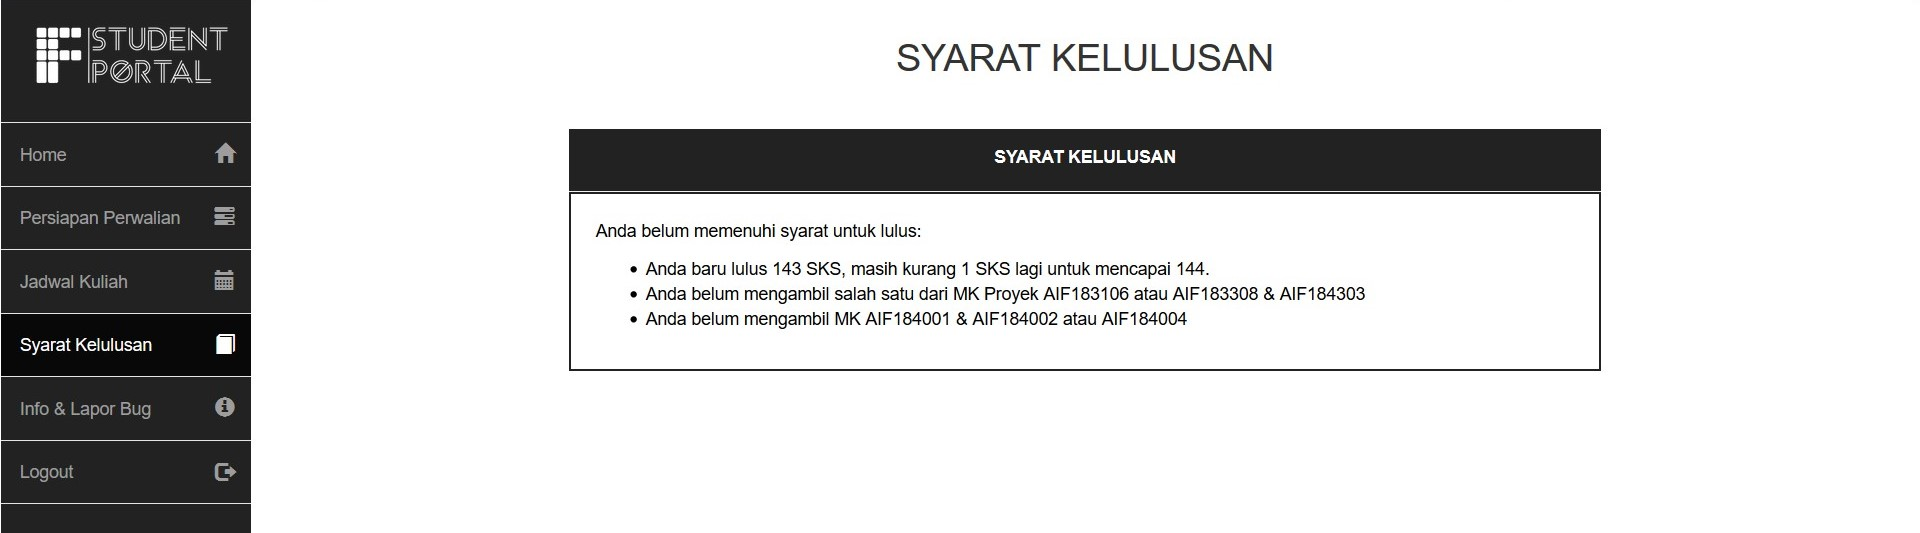
\includegraphics[scale=0.425]{Gambar/HasilPengujian/2013_1_syarat_kelulusan_ifstudentportal}
			\caption{Halaman Syarat Kelulusan (IFStudentPortal) - Steven Haryanto}
			\label{fig:2013_1_syarat_kelulusan_ifstudentportal}
		\end{figure}
		\begin{figure}[H]
			\centering
			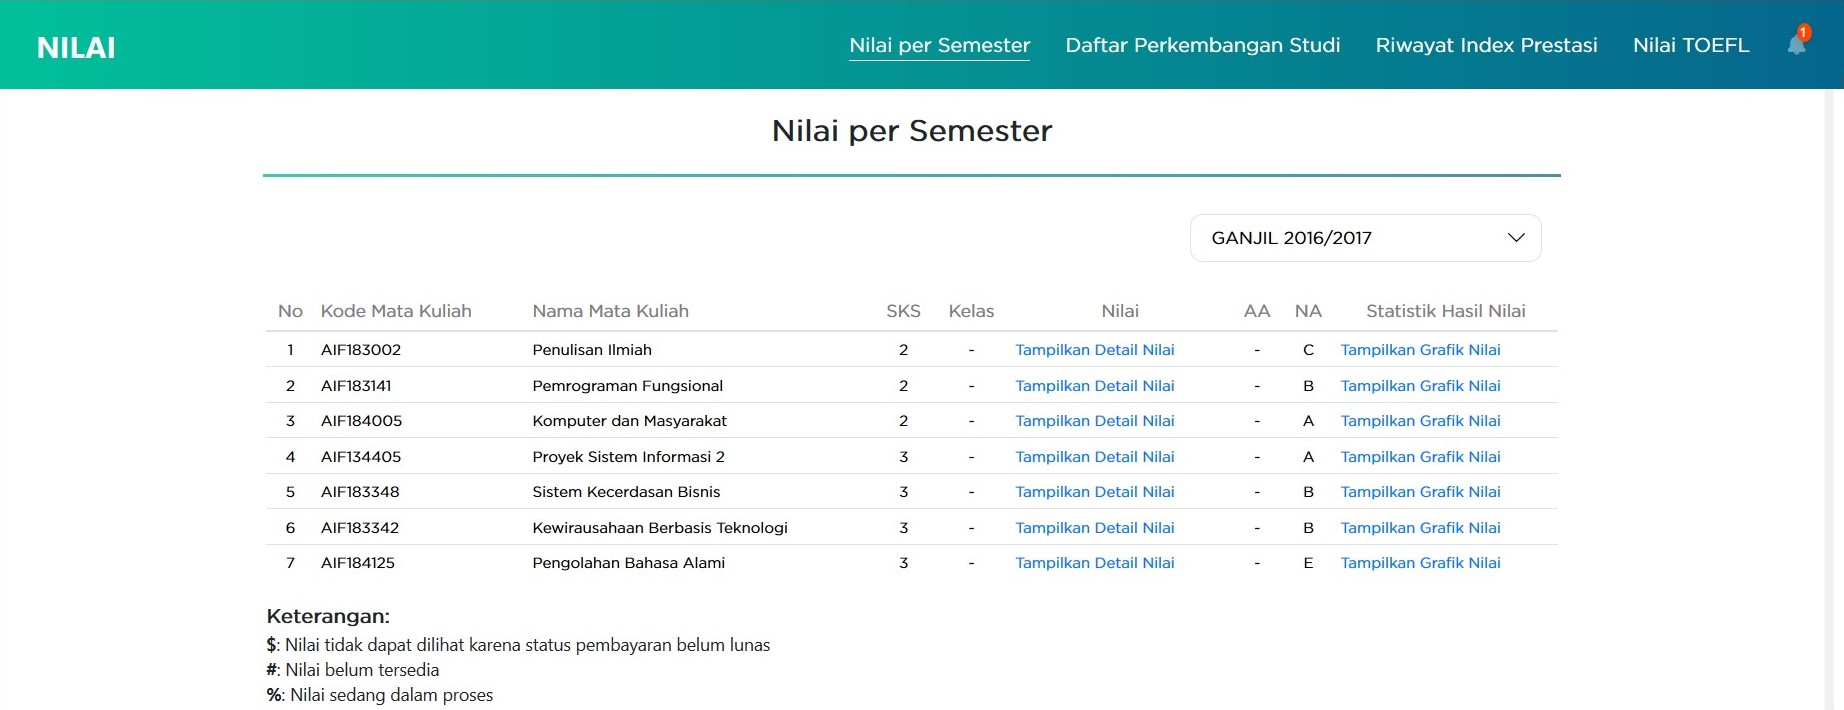
\includegraphics[scale=0.4]{Gambar/HasilPengujian/2013_1_nps_studentportal}
			\caption{Halaman Nilai Per Semester (Student Portal) - Steven Haryanto}
			\label{fig:2013_1_nps_studentportal}
		\end{figure}
		\begin{figure}[H]
			\centering
			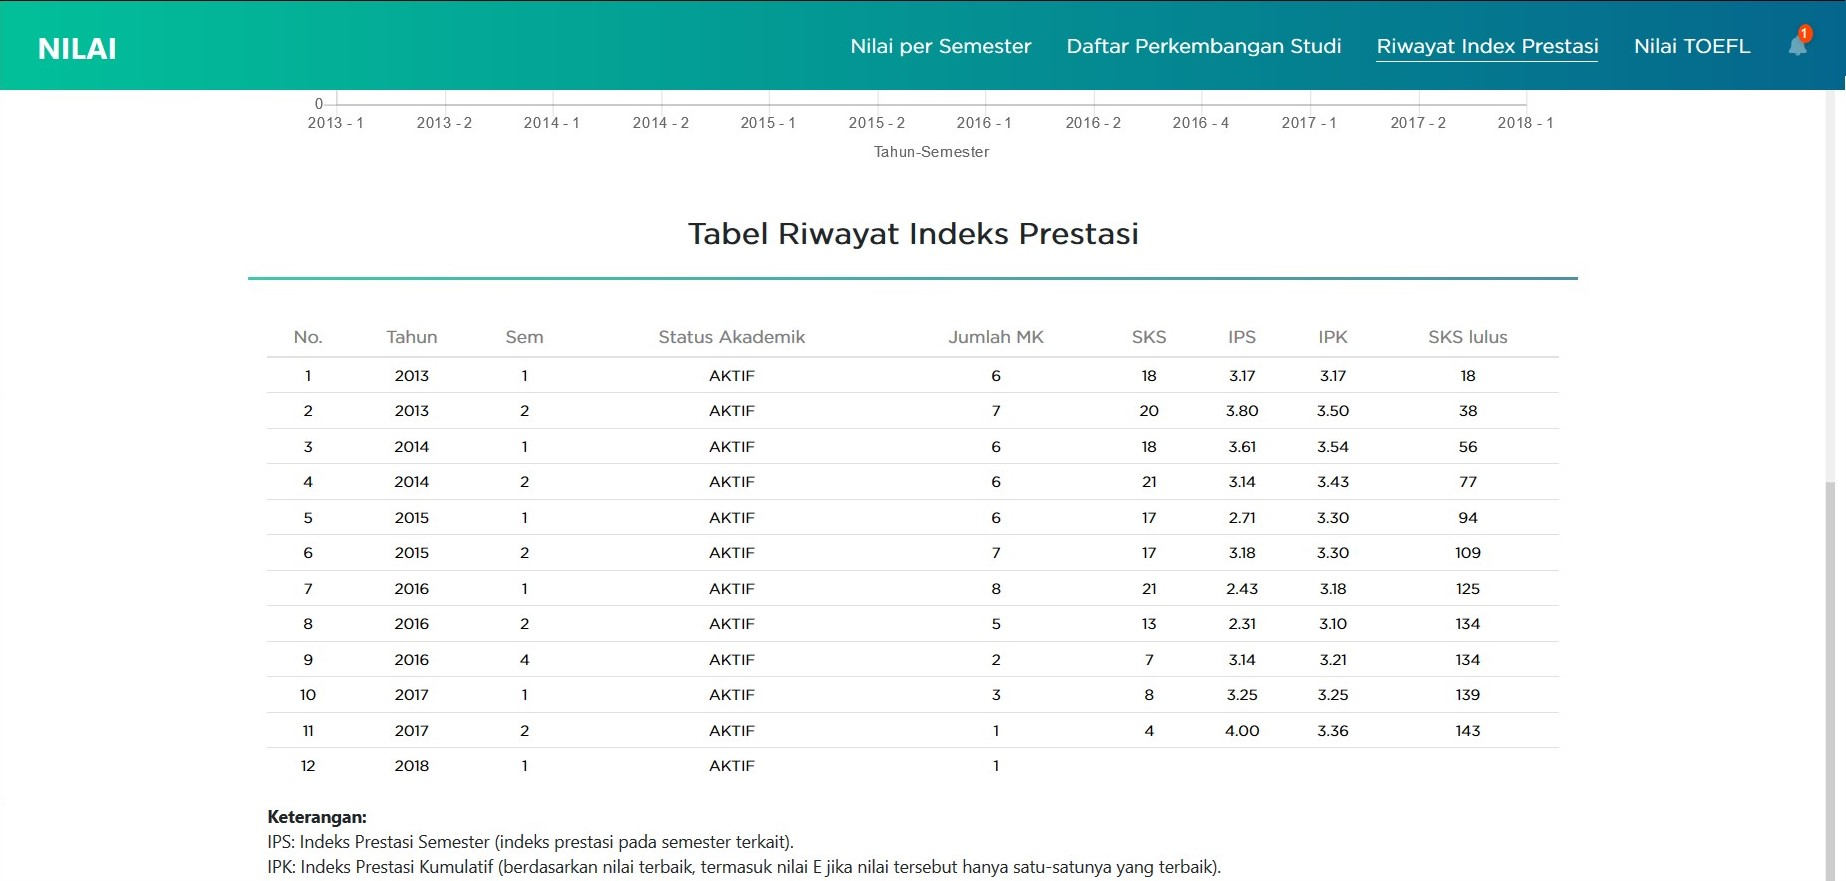
\includegraphics[scale=0.4]{Gambar/HasilPengujian/2013_1_rip_studentportal}
			\caption{Halaman Riwayat Indek Prestasi (Student Portal) - Steven Haryanto}
			\label{fig:2013_1_rip_studentportal}
		\end{figure}
		\begin{figure}[H]
			\centering
			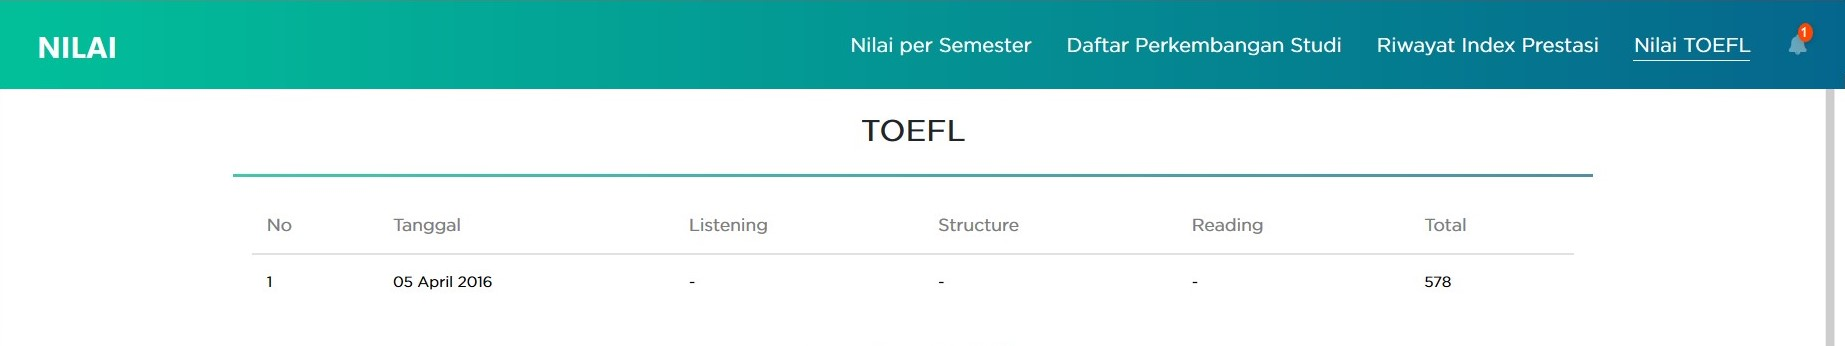
\includegraphics[scale=0.4]{Gambar/HasilPengujian/2013_1_toefl_studentportal}
			\caption{Halaman Nilai TOEFL (Student Portal) - Steven Haryanto}
			\label{fig:2013_1_toefl_studentportal}
		\end{figure}
		\begin{figure}[H]
			\centering
			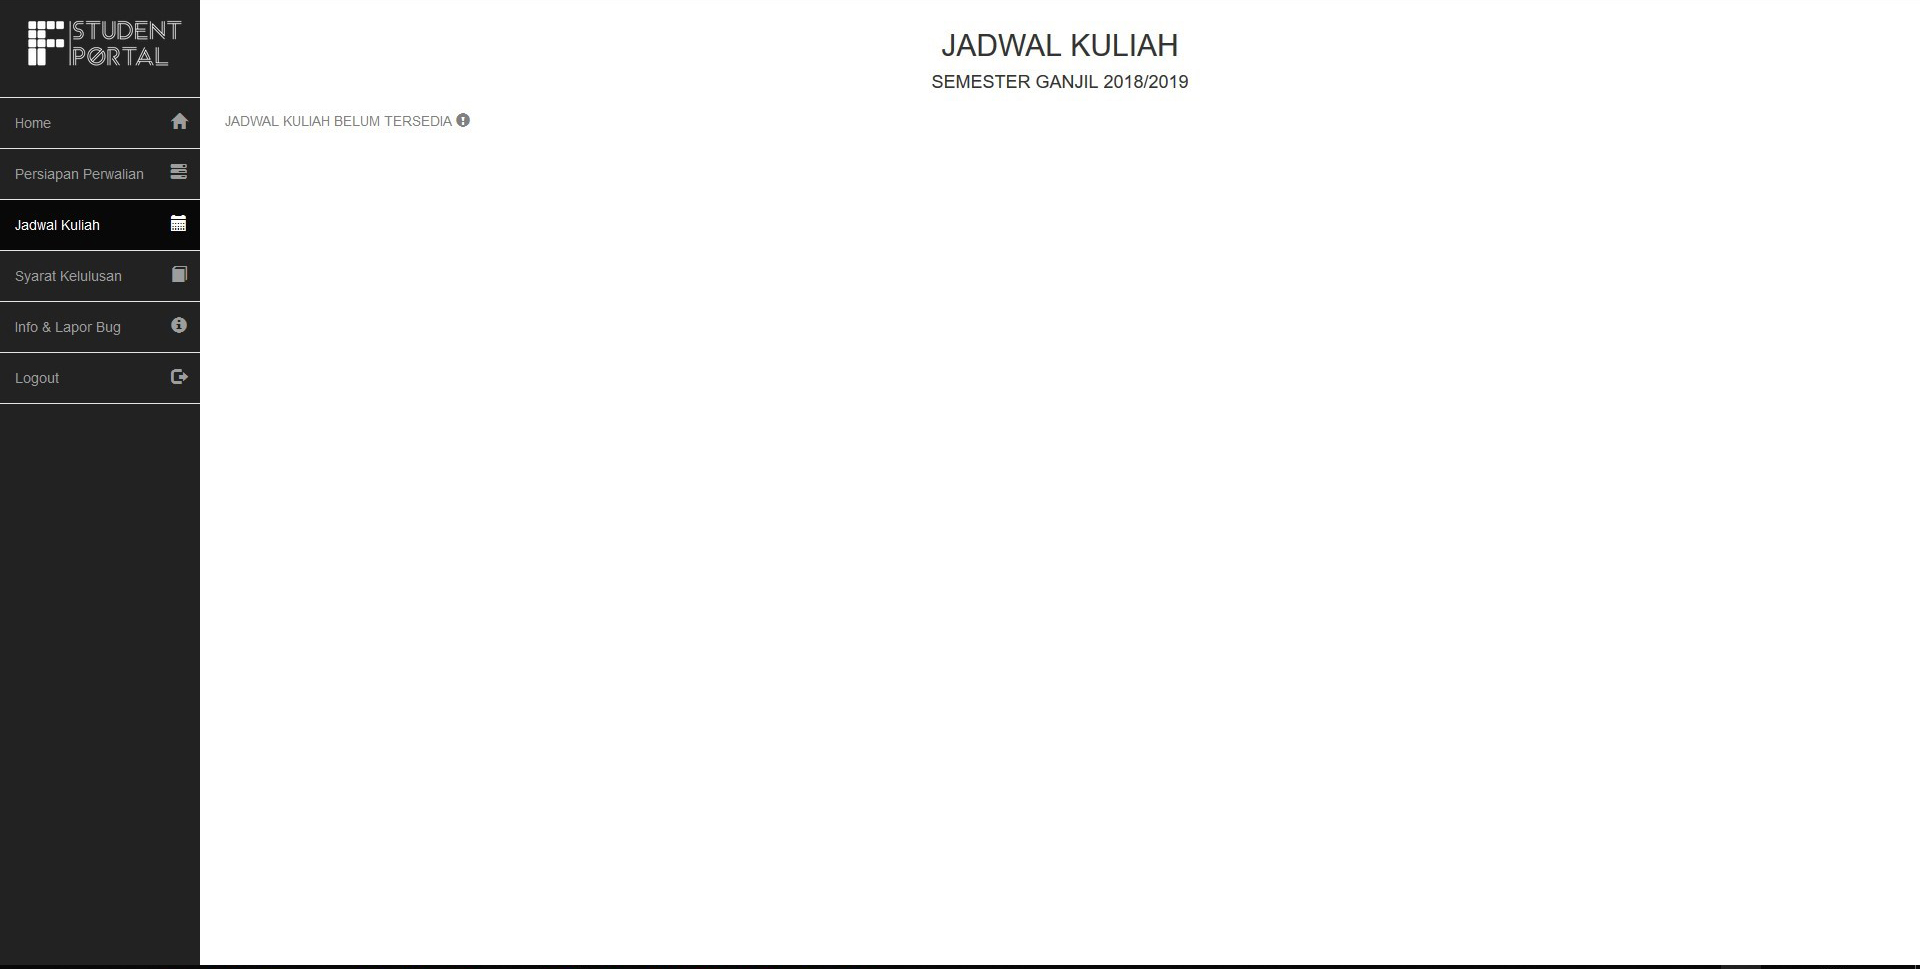
\includegraphics[scale=0.325]{Gambar/HasilPengujian/2013_1_jadwal_kuliah_ifstudentportal}
			\caption{Halaman Jadwal Kuliah (IFStudentPortal) - Steven Haryanto}
			\label{fig:2013_1_jadwal_kuliah_ifstudentportal}
		\end{figure}
		\begin{figure}[H]
			\centering
			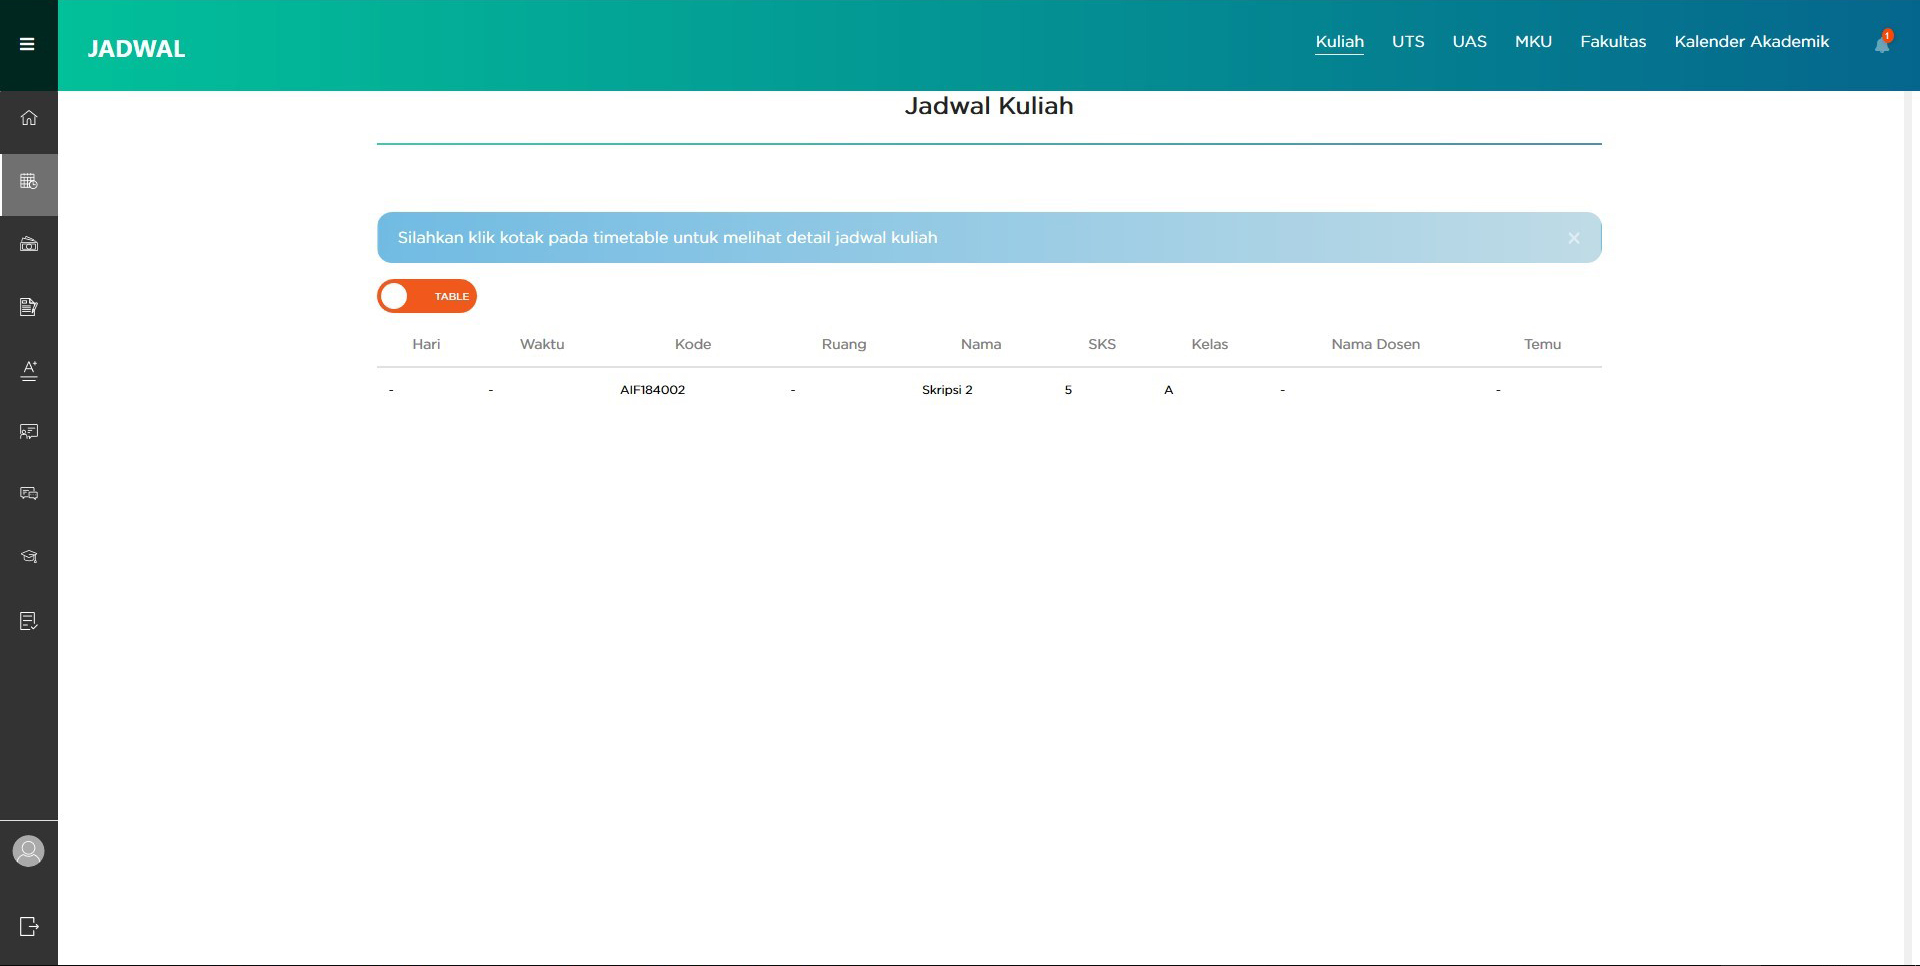
\includegraphics[scale=0.325]{Gambar/HasilPengujian/2013_1_jadwal_kuliah_studentportal}
			\caption{Halaman Jadwal Kuliah (Student Portal) - Steven Haryanto}
			\label{fig:2013_1_jadwal_kuliah_studentportal}
		\end{figure}
			Hasil pengujian eksperimental halaman persiapan perwalian dari IFStudentPortal yang berisi data akademik (IPS, IPK, IP Lulus, IP Nilai Terbaik, sks lulus, dan nilai TOEFL) dan data mata kuliah berserta prasyaratnya dapat dilihat pada Gambar \ref{fig:2013_1_persiapan_perwalian_ifstudentportal}. Gambar \ref{fig:2013_1_rip_studentportal} menunjukkan riwayat IP sedangkan Gambar \ref{fig:2013_1_nps_studentportal} menunjukkan salah satu nilai per semester mahasiswa dan Gambar \ref{fig:2013_1_toefl_studentportal} menunjukkan riwayat nilai TOEFL mahasiswa. Hasil tersebut menunjukkan bahwa halaman persiapan perwalian sudah sesuai dengan data mahasiswa pada Student Portal. Hasil pengujian berikutnya mahasiswa melakukan pemeriksaan syarat kelulusan terdapat syarat yang seharusnya sudah lulus yaitu ``Anda belum mengambil salah satu dari MK Proyek AIF183106 atau AIF183308 \& AIF184303''(Gambar \ref{fig:2013_1_syarat_kelulusan_ifstudentportal}). Hal ini disebabkan perbedaan kode mata kuliah ``Proyek Sistem Infomasi 2'' dengan \cite{dokumenkurikulum2018}. Pada \cite{dokumenkurikulum2018} dituliskan hasil transisi untuk mata kuliah ``Proyek Sistem Infomasi 2'' adalah ``AIF184303'', sedangkan pada StudentPortal adalah ``AIF134405''(Gambar \ref{fig:2013_1_nps_studentportal}). Hasil pengujian berikutnya dapat dilihat pada Gambar \ref{fig:2013_1_jadwal_kuliah_ifstudentportal} menunjukan jadwal kuliah mahasiswa pada IFStudentPortal. Kemudian jadwal kuliah mahasiswa pada Student Portal dapat dilihat pada Gambar \ref{fig:2013_1_jadwal_kuliah_studentportal}. Hasil tersebut menunjukkan bahwa jadwal kuliah dari IFStudentPortal sudah sesuai dengan jadwal kuliah pada Student Portal.
		\item Harseto Pandityo - 2013730060 \\
		\begin{figure}[H]
			\centering
			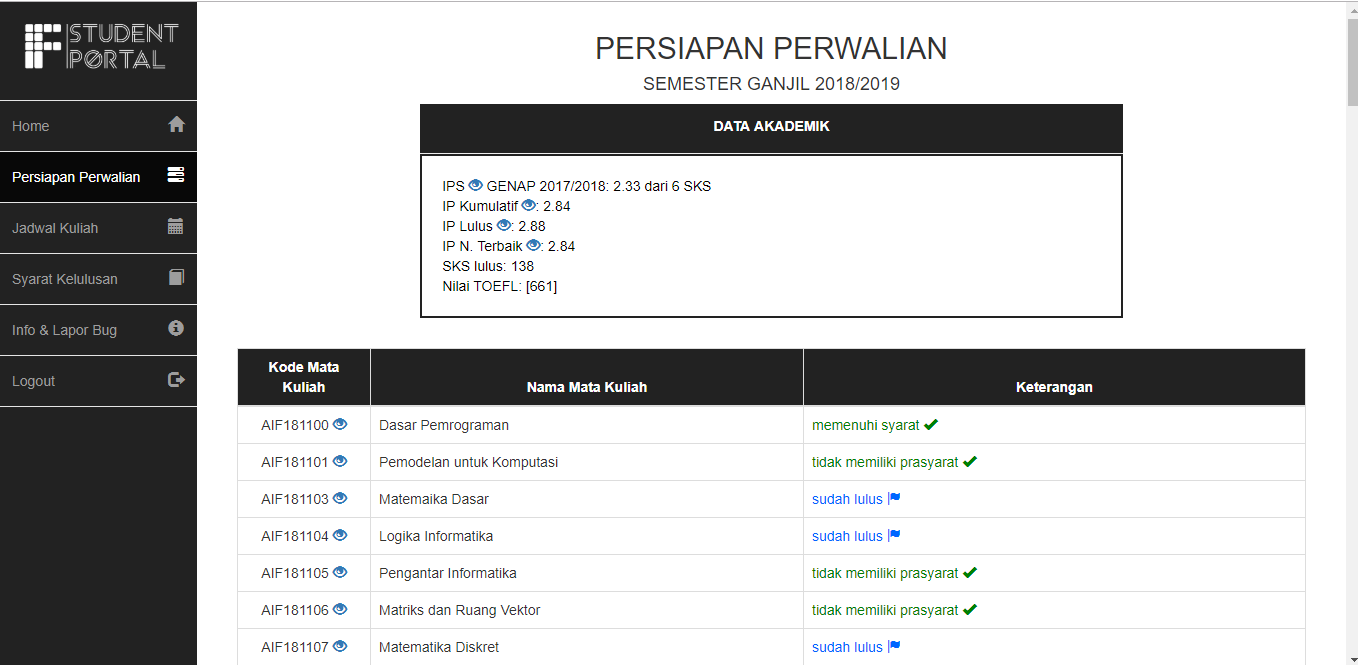
\includegraphics[scale=0.45]{Gambar/HasilPengujian/2013_2_persiapan_perwalian_ifstudentportal}
			\caption{Halaman Persiapan Perwalian (IFStudentPortal) - Harseto Pandityo}
			\label{fig:2013_2_persiapan_perwalian_ifstudentportal}
		\end{figure}
		\begin{figure}[H]
			\centering
			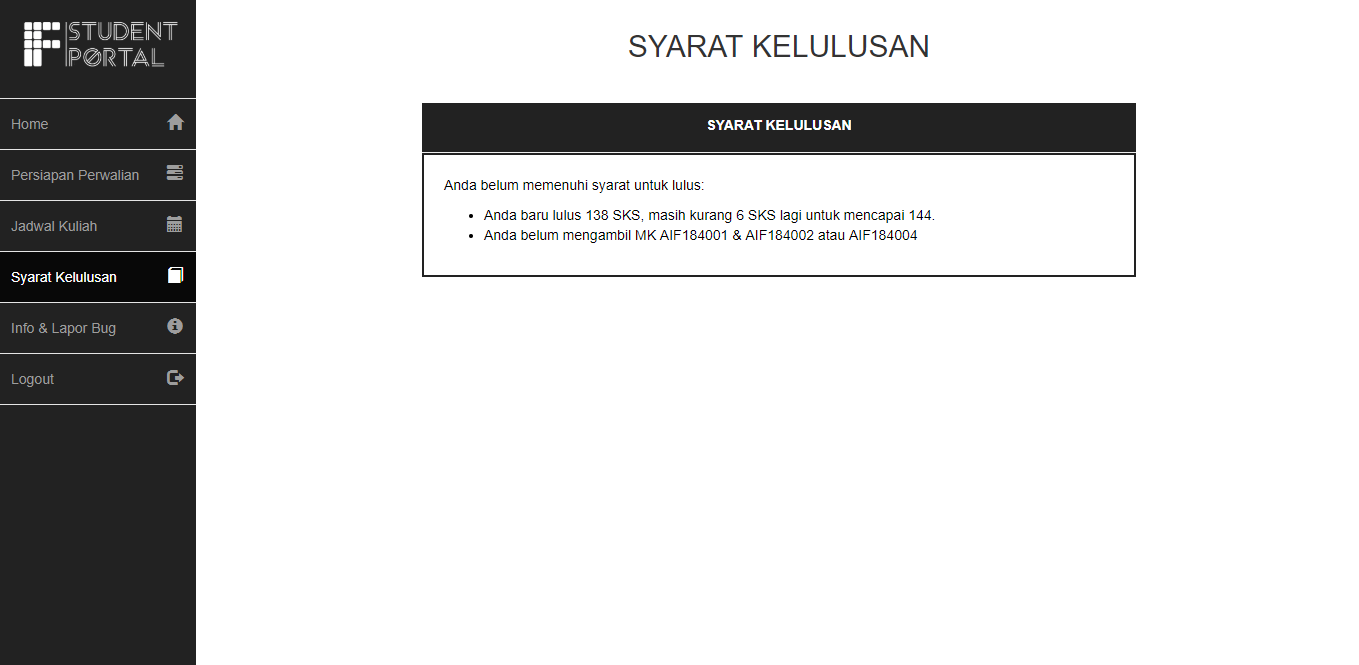
\includegraphics[scale=0.45]{Gambar/HasilPengujian/2013_2_syarat_kelulusan_ifstudentportal}
			\caption{Halaman Syarat Kelulusan (IFStudentPortal) - Harseto Pandityo}
			\label{fig:2013_2_syarat_kelulusan_ifstudentportal}
		\end{figure}
		\begin{figure}[H]
			\centering
			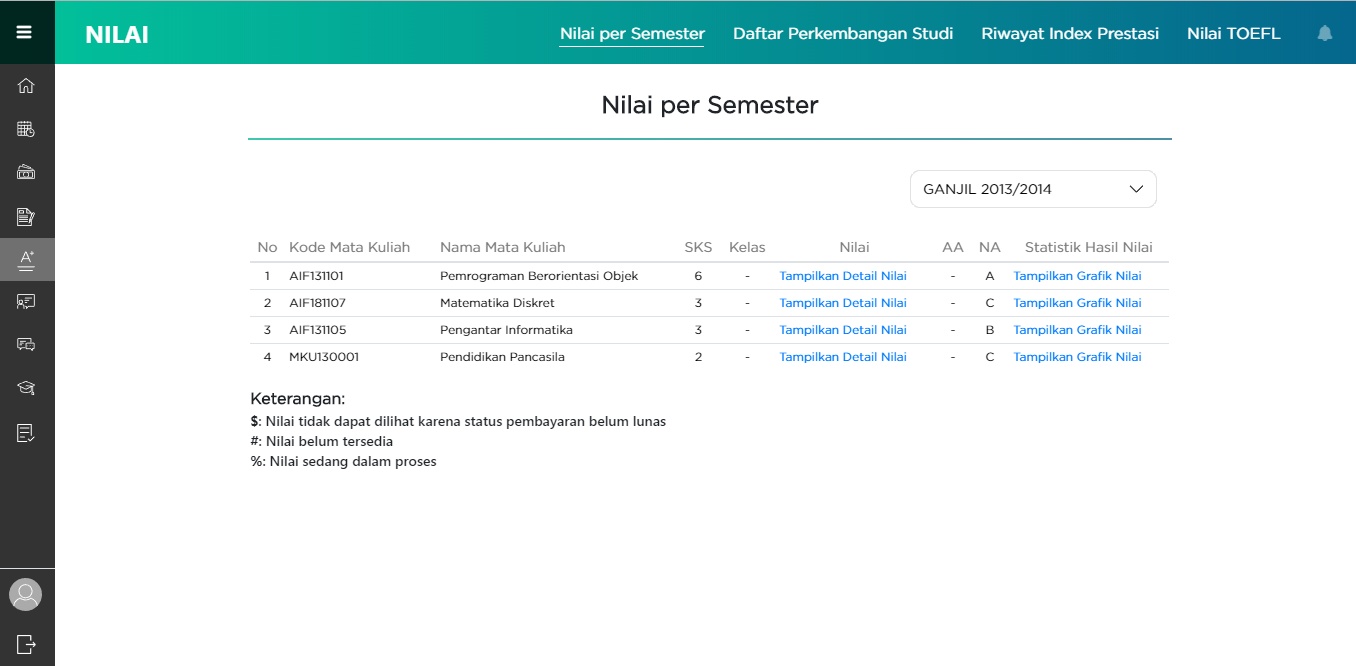
\includegraphics[scale=0.45]{Gambar/HasilPengujian/2013_2_nps_studentportal}
			\caption{Halaman Nilai Per Semester (Student Portal) - Harseto Pandityo}
			\label{fig:2013_2_nps_studentportal}
		\end{figure}
		\begin{figure}[H]
			\centering
			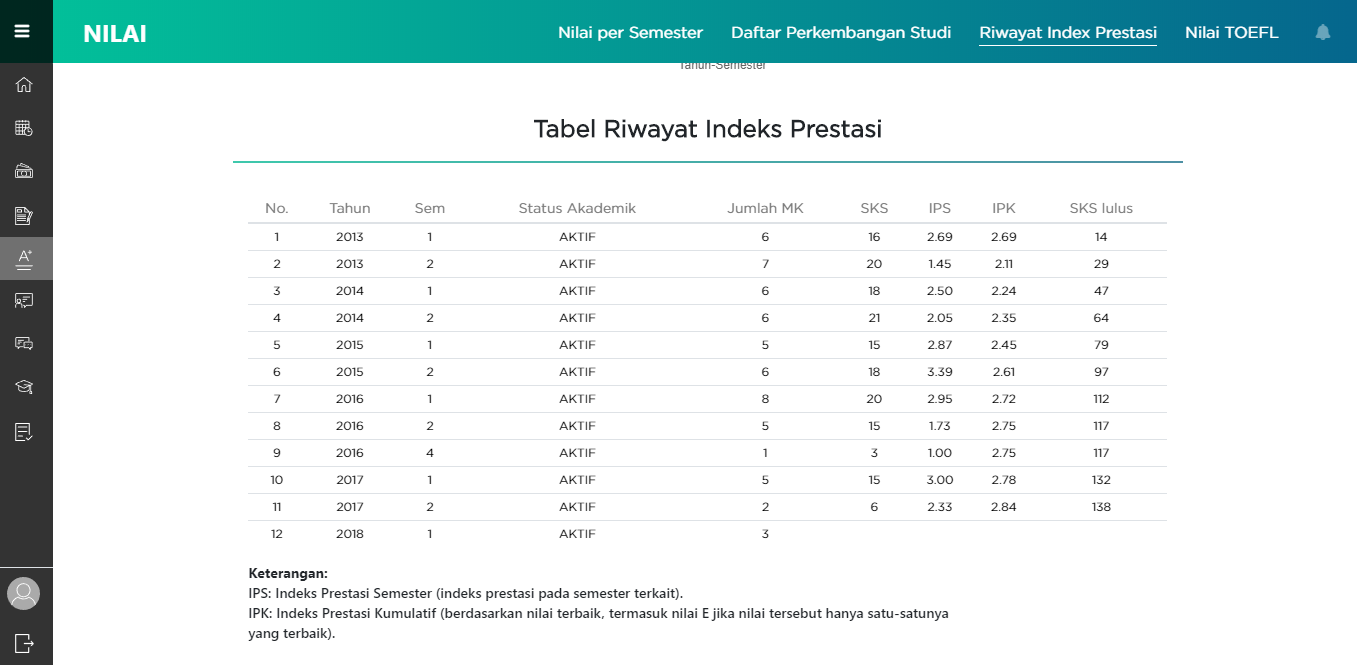
\includegraphics[scale=0.45]{Gambar/HasilPengujian/2013_2_rip_studentportal}
			\caption{Halaman Riwayat Indek Prestasi (Student Portal) - Harseto Pandityo}
			\label{fig:2013_2_rip_studentportal}
		\end{figure}
		\begin{figure}[H]
			\centering
			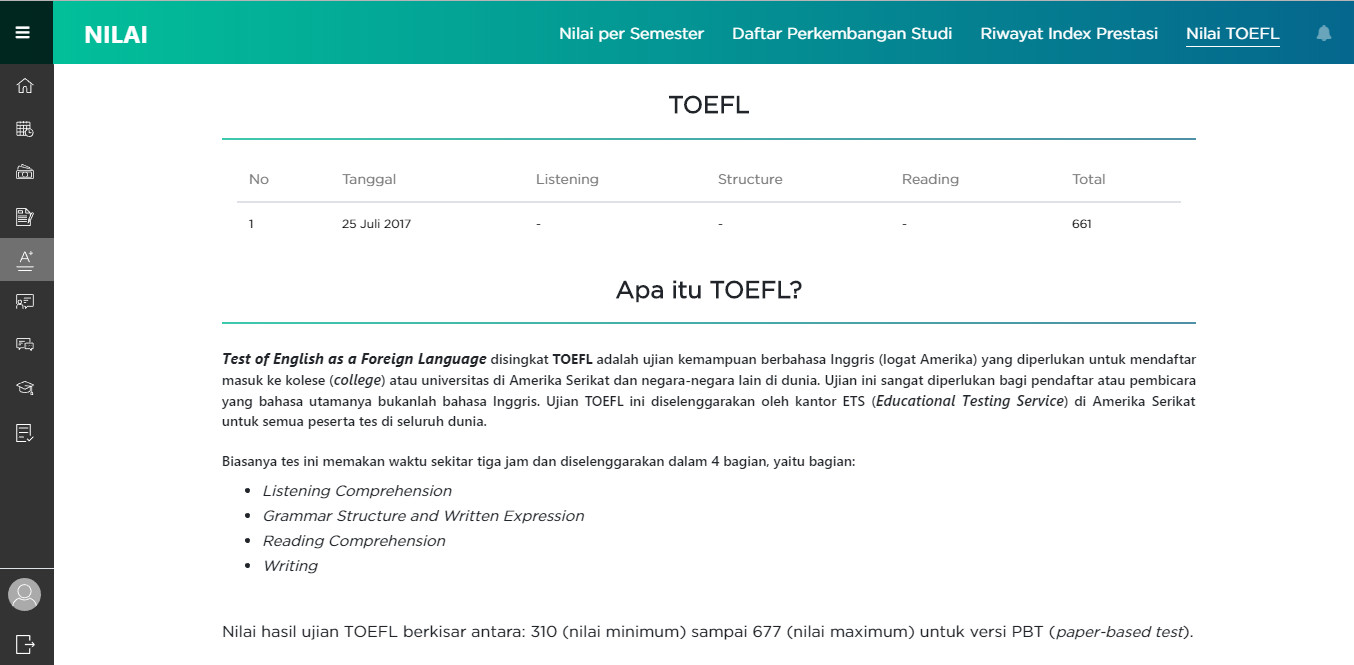
\includegraphics[scale=0.45]{Gambar/HasilPengujian/2013_2_toefl_studentportal}
			\caption{Halaman Nilai TOEFL (Student Portal) - Harseto Pandityo}
			\label{fig:2013_2_toefl_studentportal}
		\end{figure}
		\begin{figure}[H]
			\centering
			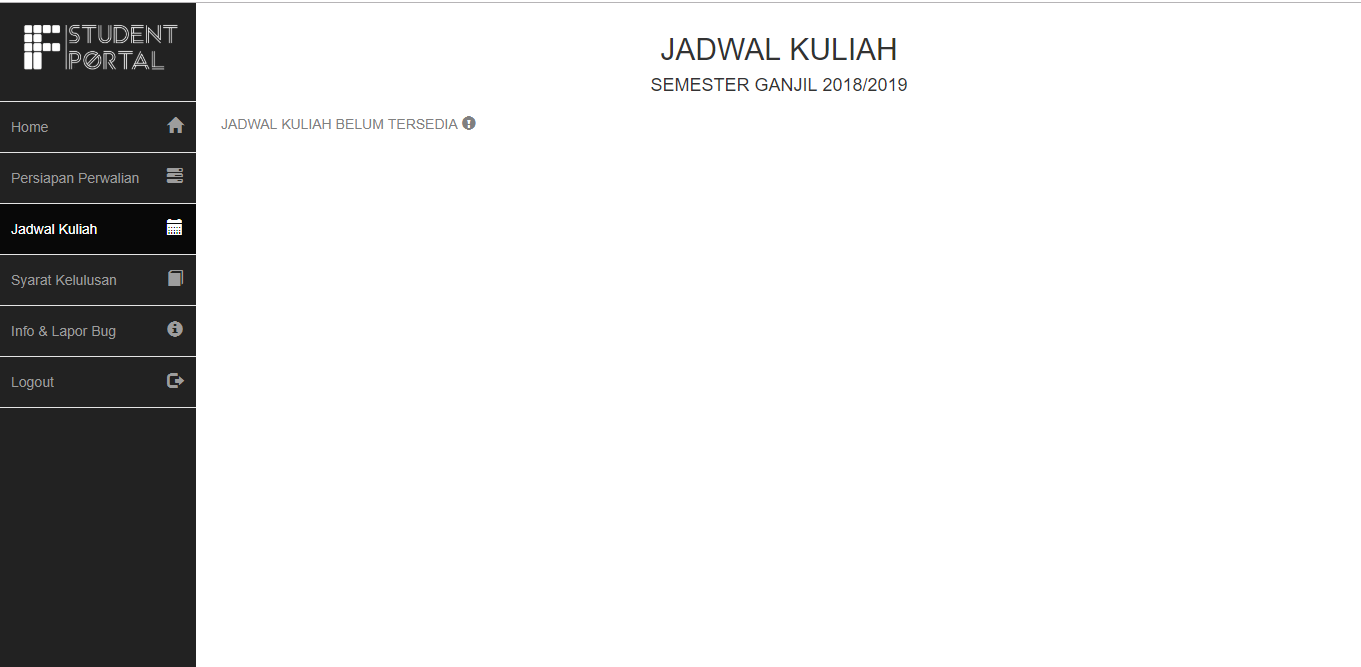
\includegraphics[scale=0.45]{Gambar/HasilPengujian/2013_2_jadwal_kuliah_ifstudentportal}
			\caption{Halaman Jadwal Kuliah (IFStudentPortal) - Harseto Pandityo}
			\label{fig:2013_2_jadwal_kuliah_ifstudentportal}
		\end{figure}
		\begin{figure}[H]
			\centering
			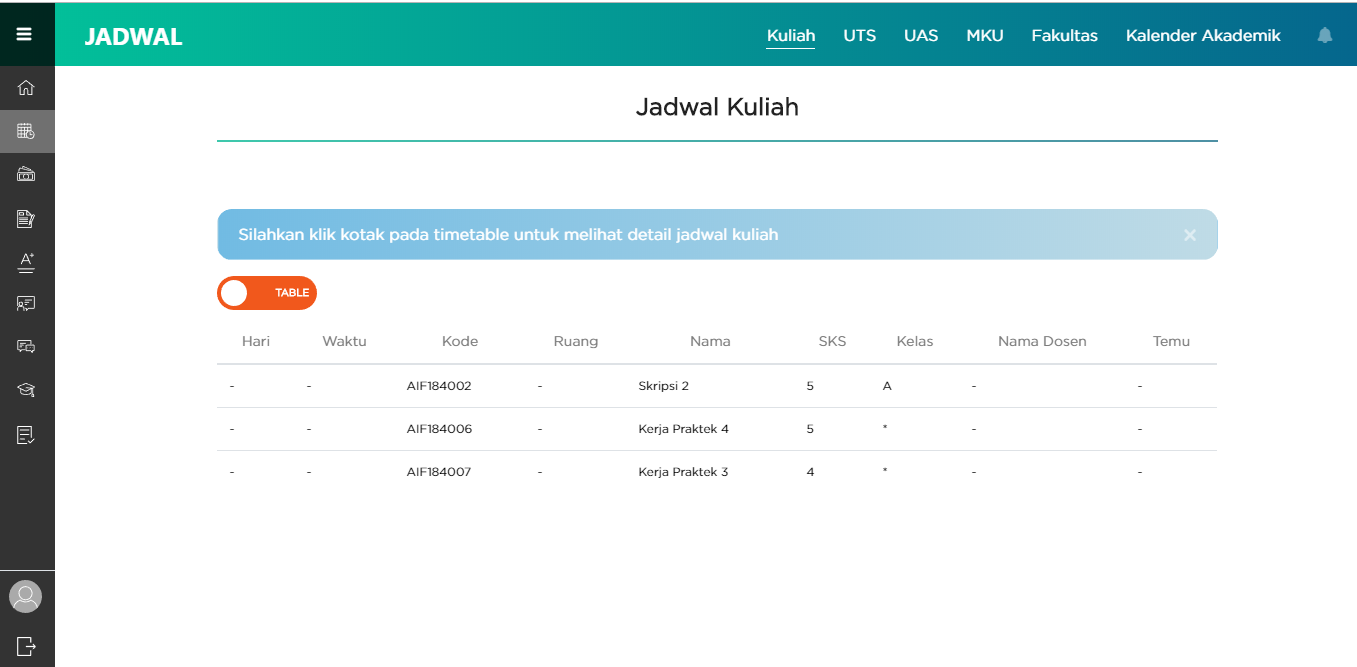
\includegraphics[scale=0.45]{Gambar/HasilPengujian/2013_2_jadwal_kuliah_studentportal}
			\caption{Halaman Jadwal Kuliah (Student Portal) - Harseto Pandityo}
			\label{fig:2013_2_jadwal_kuliah_studentportal}
		\end{figure}
		Hasil pengujian eksperimental halaman persiapan perwalian dari IFStudentPortal yang berisi data akademik (IPS, IPK, IP Lulus, IP Nilai Terbaik, sks lulus, dan nilai TOEFL) dan data mata kuliah berserta prasyaratnya dapat dilihat pada Gambar \ref{fig:2013_2_persiapan_perwalian_ifstudentportal}. Gambar \ref{fig:2013_2_rip_studentportal} menunjukkan riwayat IP sedangkan Gambar \ref{fig:2013_2_nps_studentportal} menunjukkan salah satu nilai per semester mahasiswa dan Gambar \ref{fig:2013_1_toefl_studentportal} menunjukkan riwayat nilai TOEFL mahasiswa. Hasil tersebut menunjukkan bahwa halaman persiapan perwalian sudah sesuai dengan data mahasiswa pada Student Portal. Hasil pengujian berikutnya dapat dilihat pada Gambar \ref{fig:2013_2_syarat_kelulusan_ifstudentportal} menujukkan syarat lulus mahasiswa Teknik Informatika UNPAR sedangkan Gambar \ref{fig:2013_2_nps_studentportal} menujukkan salah satu data nilai hasil transisi ke kurikulum 2018. Hasil tersebut menunjukkan bahwa halaman syarat kelulusan telah sesuai dengan hasil yang diharapkan. Hasil pengujian berikutnya dapat dilihat pada Gambar \ref{fig:2013_2_jadwal_kuliah_ifstudentportal} menunjukan jadwal kuliah mahasiswa pada IFStudentPortal. Kemudian jadwal kuliah mahasiswa pada Student Portal dapat dilihat pada Gambar \ref{fig:2013_2_jadwal_kuliah_studentportal}. Hasil tersebut menunjukkan bahwa jadwal kuliah dari IFStudentPortal sudah sesuai dengan jadwal kuliah pada Student Portal.
	\end{enumerate}
	Hasil pengujian eksperimental dari kedua mahasiswa angkatan 2013 sesuai dengan hasil yang diharapkan.
	\item Angkatan 2014 \\
	Untuk angkatan 2014 pengujian dilakukan kepada dua orang mahasiswa, yaitu:
	\begin{enumerate}
		\item Fedrian Hermana - 2014730008
		\begin{figure}[H]
			\centering
			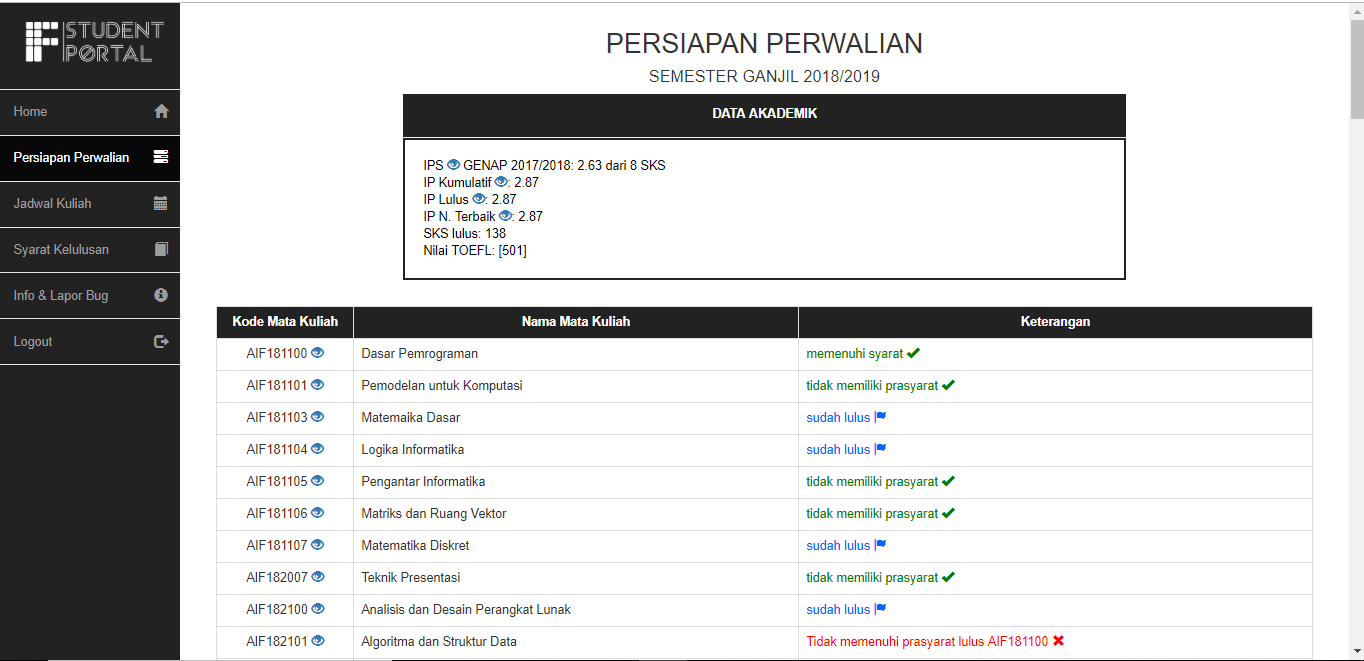
\includegraphics[scale=0.45]{Gambar/HasilPengujian/2014_1_persiapan_perwalian_ifstudentportal}
			\caption{Halaman Persiapan Perwalian (IFStudentPortal) - Fedrian Hermana}
			\label{fig:2014_1_persiapan_perwalian_ifstudentportal}
		\end{figure}
		\begin{figure}[H]
			\centering
			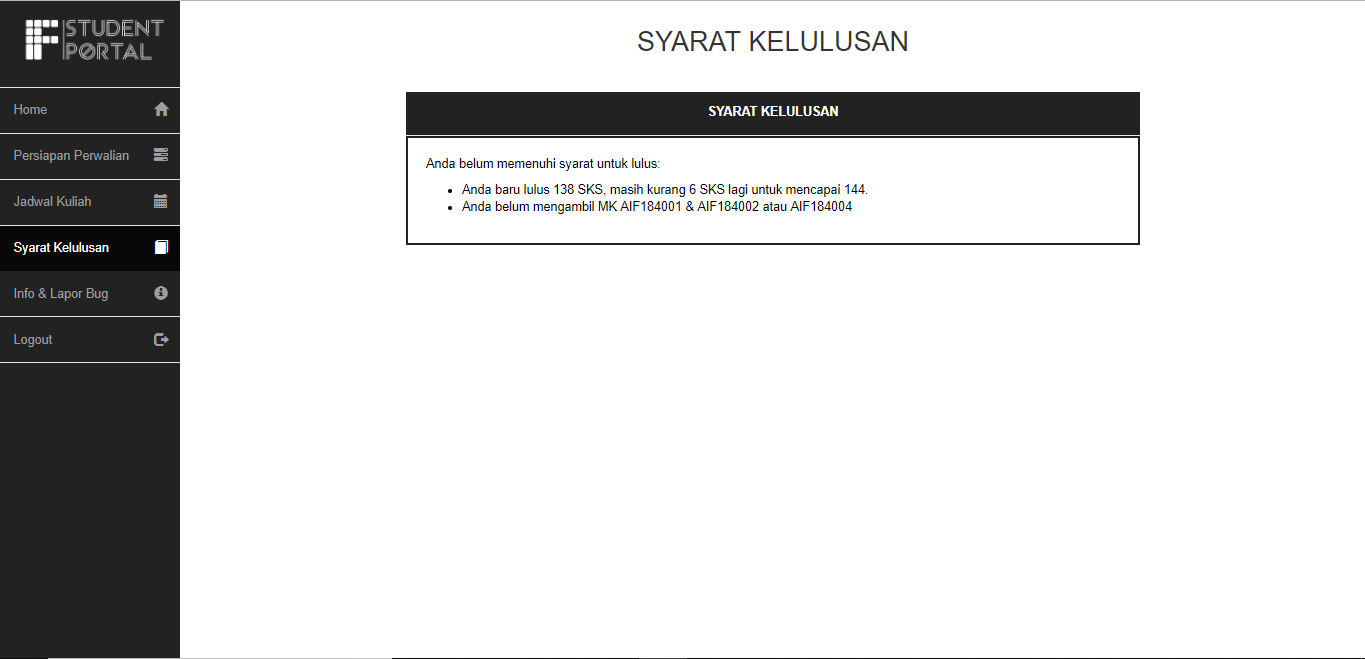
\includegraphics[scale=0.45]{Gambar/HasilPengujian/2014_1_syarat_kelulusan_ifstudentportal}
			\caption{Halaman Syarat Kelulusan (IFStudentPortal) - Fedrian Hermana}
			\label{fig:2014_1_syarat_kelulusan_ifstudentportal}
		\end{figure}
		\begin{figure}[H]
			\centering
			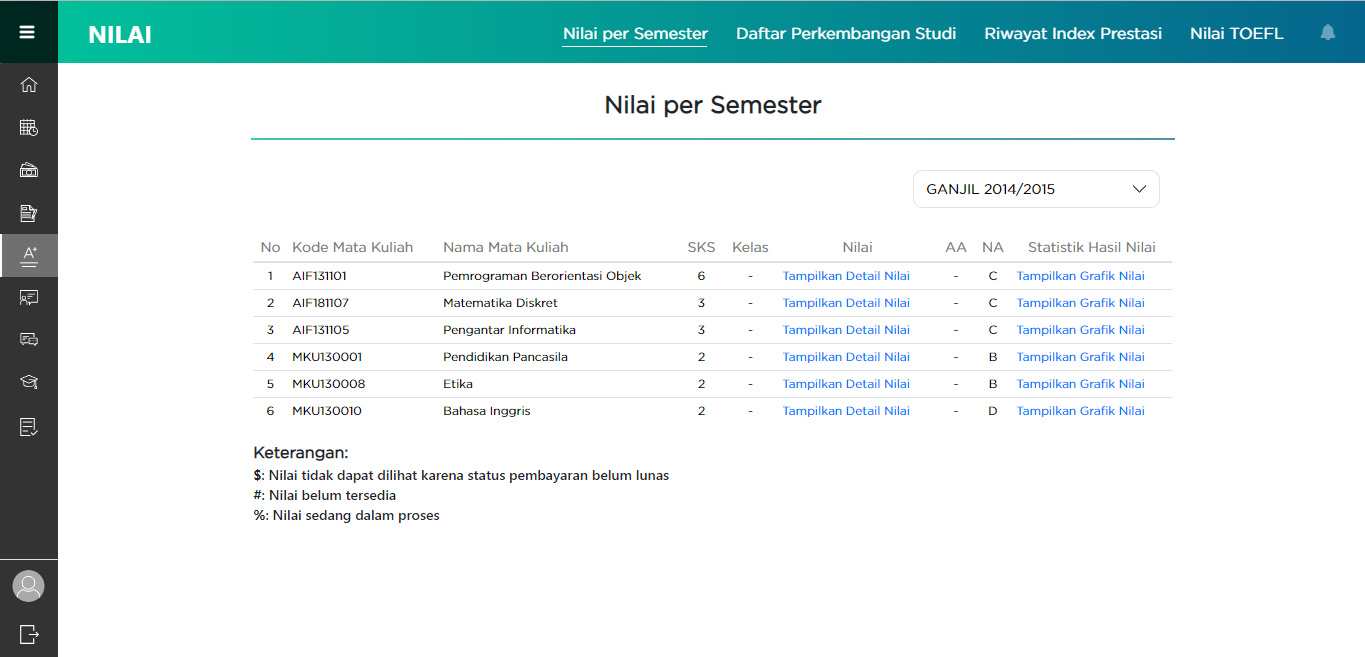
\includegraphics[scale=0.45]{Gambar/HasilPengujian/2014_1_nps_studentportal}
			\caption{Halaman Nilai Per Semester (Student Portal) - Fedrian Hermana}
			\label{fig:2014_1_nps_studentportal}
		\end{figure}
		\begin{figure}[H]
			\centering
			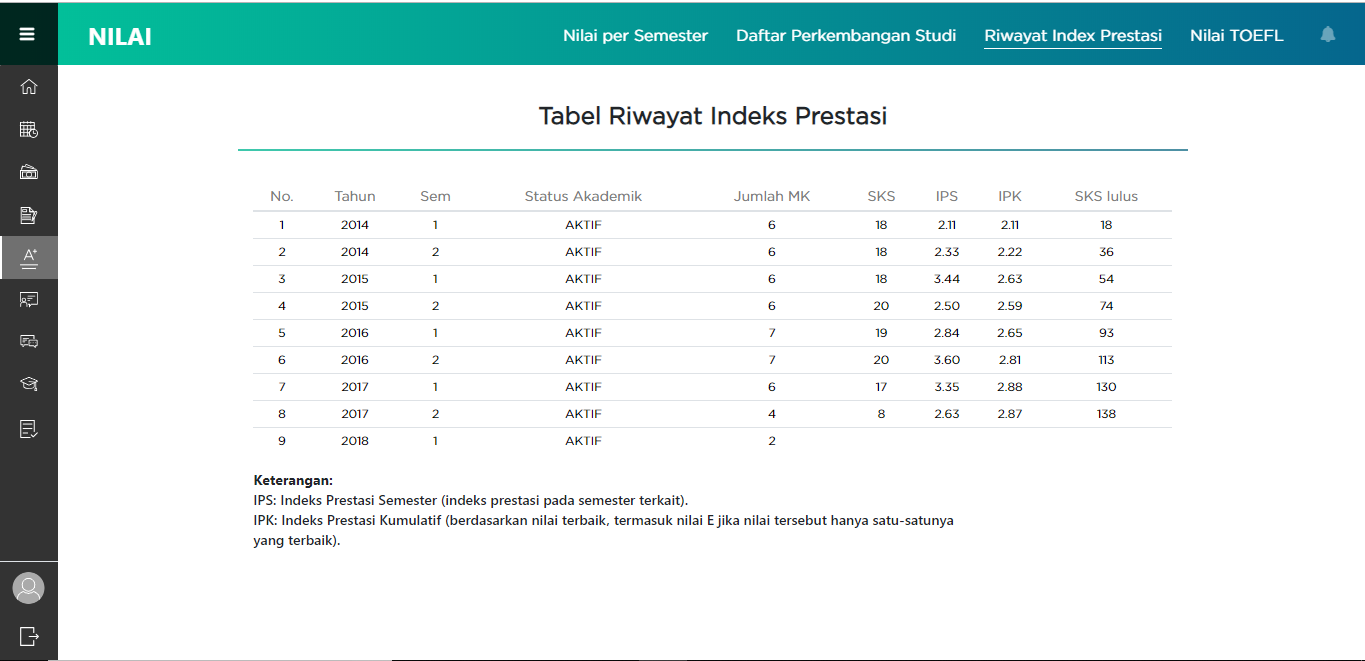
\includegraphics[scale=0.45]{Gambar/HasilPengujian/2014_1_rip_studentportal}
			\caption{Halaman Riwayat Indek Prestasi (Student Portal) - Fedrian Hermana}
			\label{fig:2014_1_rip_studentportal}
		\end{figure}
		\begin{figure}[H]
			\centering
			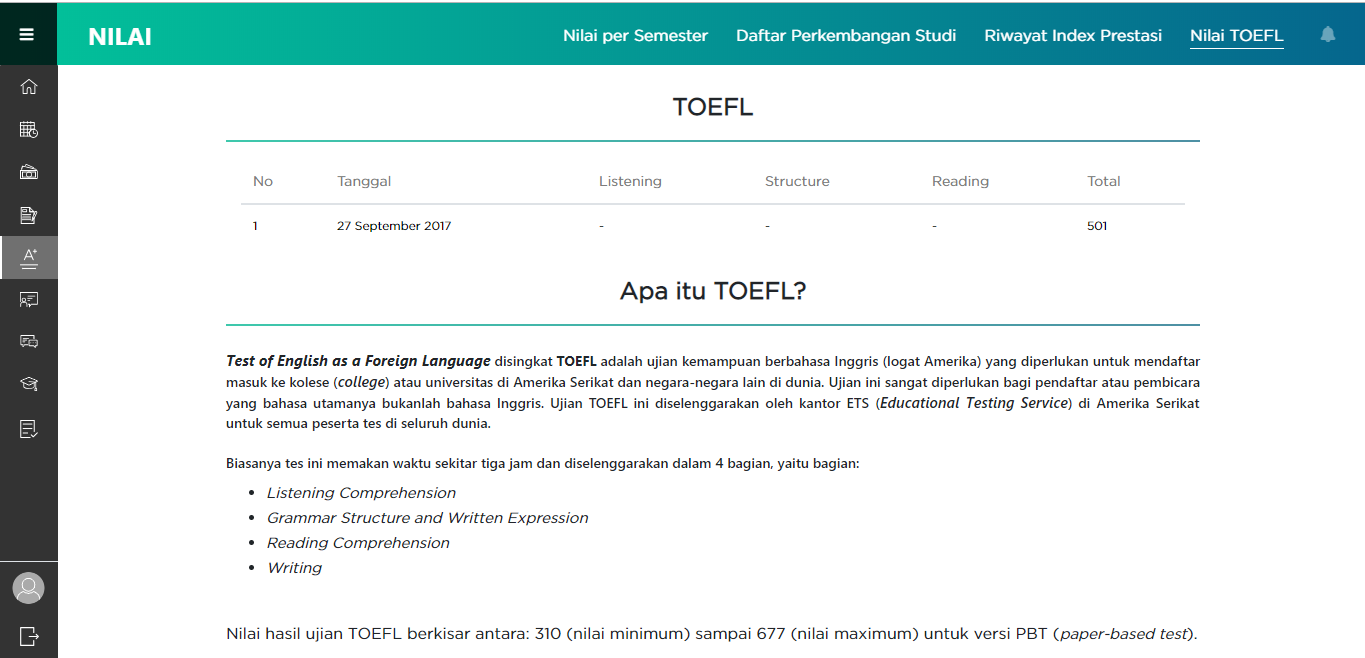
\includegraphics[scale=0.45]{Gambar/HasilPengujian/2014_1_toefl_studentportal}
			\caption{Halaman Nilai TOEFL (Student Portal) - Fedrian Hermana}
			\label{fig:2014_1_toefl_studentportal}
		\end{figure}
		\begin{figure}[H]
			\centering
			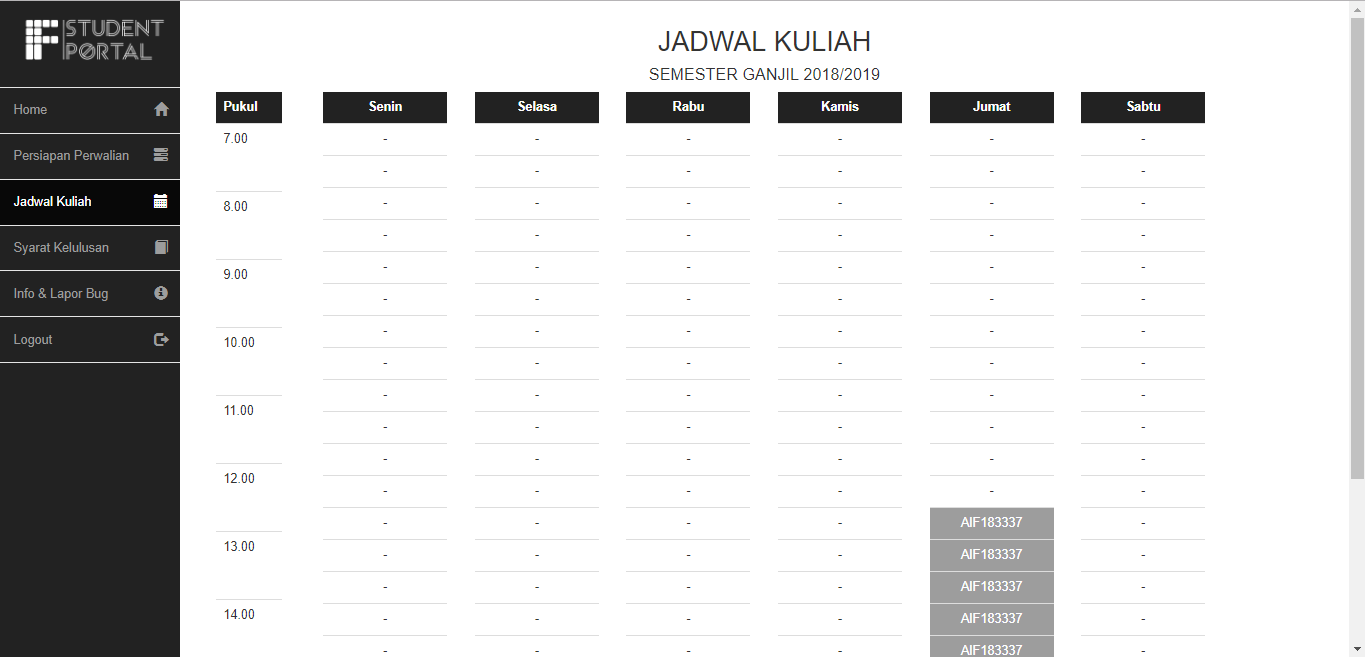
\includegraphics[scale=0.45]{Gambar/HasilPengujian/2014_1_jadwal_kuliah_ifstudentportal}
			\caption{Halaman Jadwal Kuliah (IFStudentPortal) - Fedrian Hermana}
			\label{fig:2014_1_jadwal_kuliah_ifstudentportal}
		\end{figure}
		\begin{figure}[H]
			\centering
			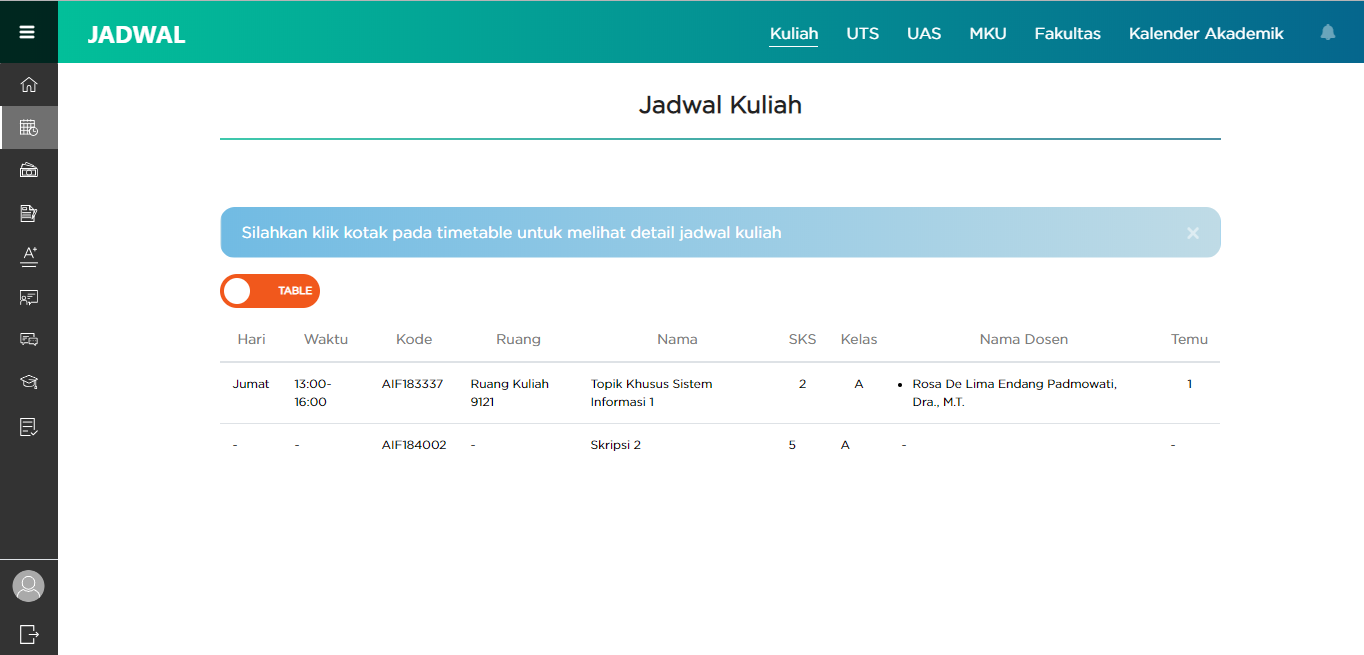
\includegraphics[scale=0.45]{Gambar/HasilPengujian/2014_1_jadwal_kuliah_studentportal}
			\caption{Halaman Jadwal Kuliah (Student Portal) - Fedrian Hermana}
			\label{fig:2014_1_jadwal_kuliah_studentportal}
		\end{figure}
		Hasil pengujian eksperimental halaman persiapan perwalian dari IFStudentPortal yang berisi data akademik (IPS, IPK, IP Lulus, IP Nilai Terbaik, sks lulus, dan nilai TOEFL) dan data mata kuliah berserta prasyaratnya dapat dilihat pada Gambar \ref{fig:2014_1_persiapan_perwalian_ifstudentportal}. Gambar \ref{fig:2014_1_rip_studentportal} menunjukkan riwayat IP sedangkan Gambar \ref{fig:2014_1_nps_studentportal} menunjukkan salah satu nilai per semester mahasiswa dan Gambar \ref{fig:2014_1_toefl_studentportal} menunjukkan riwayat nilai TOEFL mahasiswa. Hasil tersebut menunjukkan bahwa halaman persiapan perwalian sudah sesuai dengan data mahasiswa pada Student Portal. Hasil pengujian berikutnya dapat dilihat pada Gambar \ref{fig:2014_1_syarat_kelulusan_ifstudentportal} menujukkan syarat lulus mahasiswa Teknik Informatika UNPAR sedangkan Gambar \ref{fig:2014_1_nps_studentportal} menujukkan salah satu data nilai hasil transisi ke kurikulum 2018. Hasil tersebut menunjukkan bahwa halaman syarat kelulusan telah sesuai dengan hasil yang diharapkan. Hasil pengujian berikutnya dapat dilihat pada Gambar \ref{fig:2014_1_jadwal_kuliah_ifstudentportal} menunjukan jadwal kuliah mahasiswa pada IFStudentPortal. Kemudian jadwal kuliah mahasiswa pada Student Portal dapat dilihat pada Gambar \ref{fig:2014_1_jadwal_kuliah_studentportal}. Hasil tersebut menunjukkan bahwa jadwal kuliah dari IFStudentPortal sudah sesuai dengan jadwal kuliah pada Student Portal.
		\item Elia - 2014730009
		\begin{figure}[H]
			\centering
			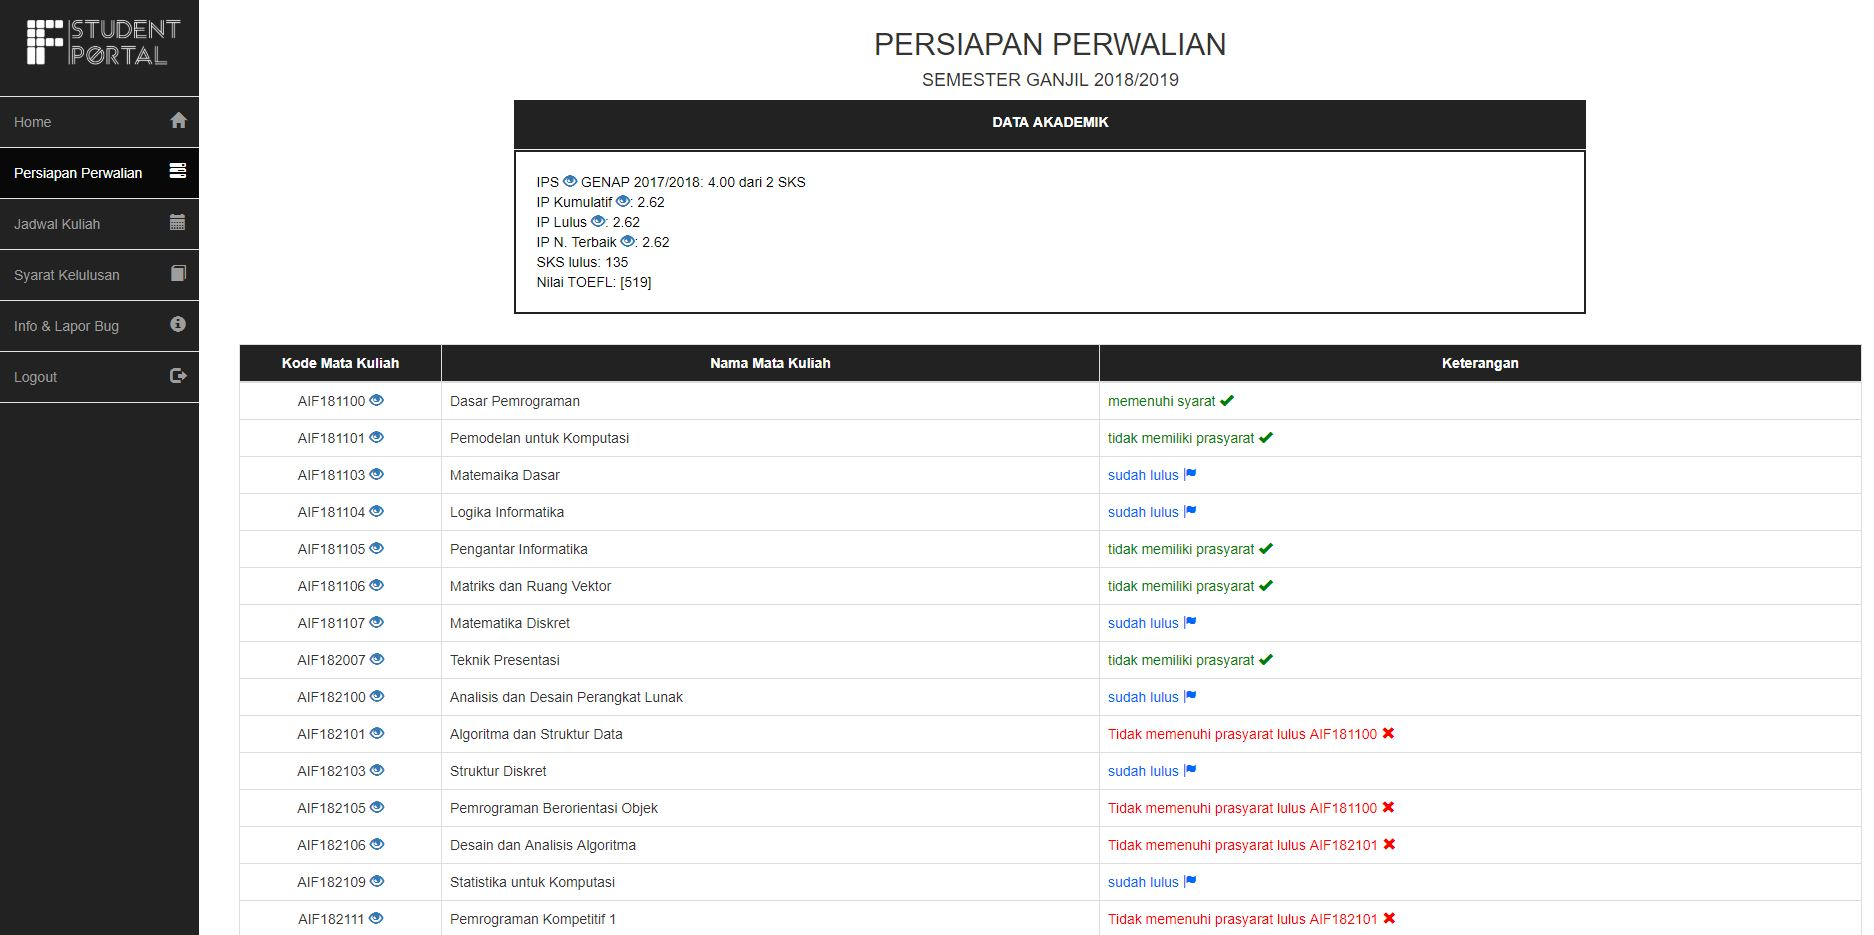
\includegraphics[scale=0.35]{Gambar/HasilPengujian/2014_2_persiapan_perwalian_ifstudentportal}
			\caption{Halaman Persiapan Perwalian (IFStudentPortal) - Elia}
			\label{fig:2014_2_persiapan_perwalian_ifstudentportal}
		\end{figure}
		\begin{figure}[H]
			\centering
			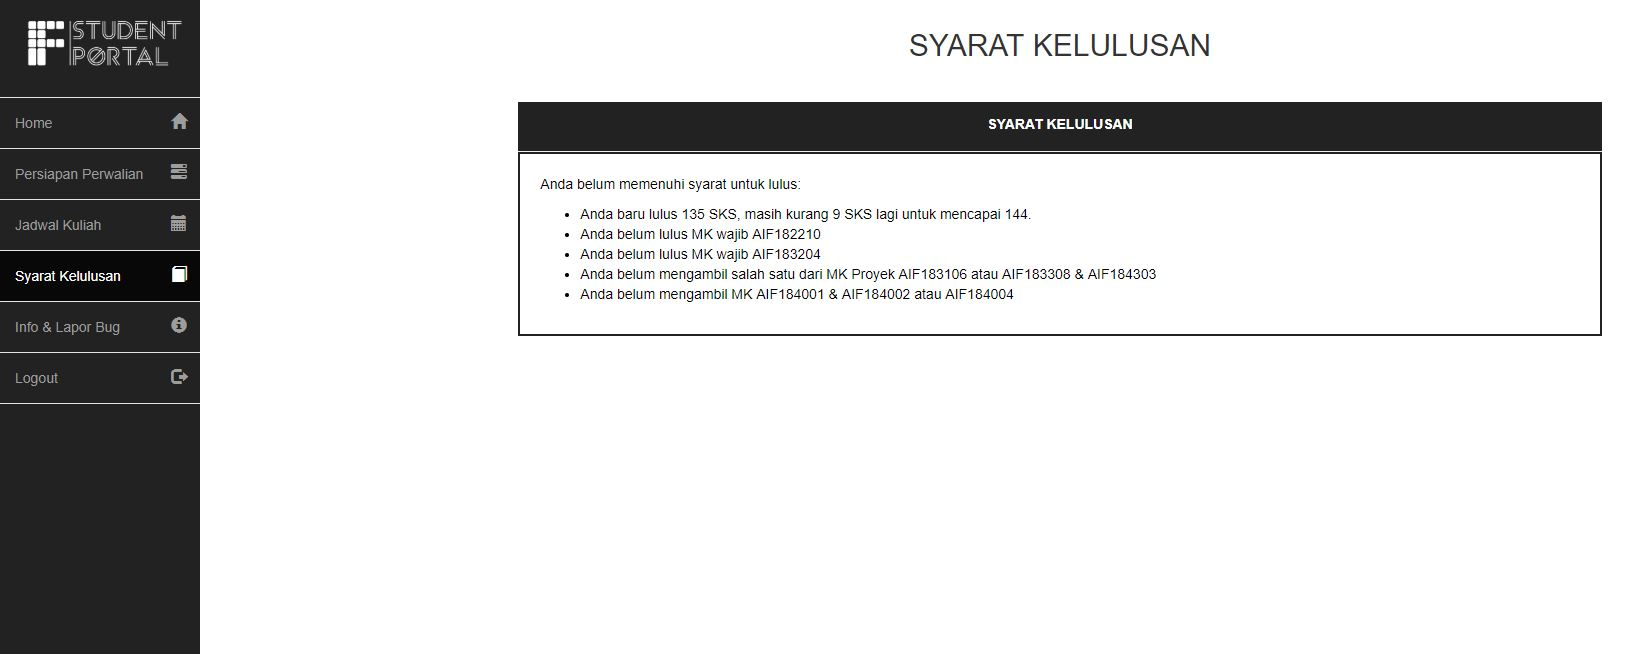
\includegraphics[scale=0.35]{Gambar/HasilPengujian/2014_2_syarat_kelulusan_ifstudentportal}
			\caption{Halaman Syarat Kelulusan (IFStudentPortal) - Elia}
			\label{fig:2014_2_syarat_kelulusan_ifstudentportal}
		\end{figure}
		\begin{figure}[H]
			\centering
			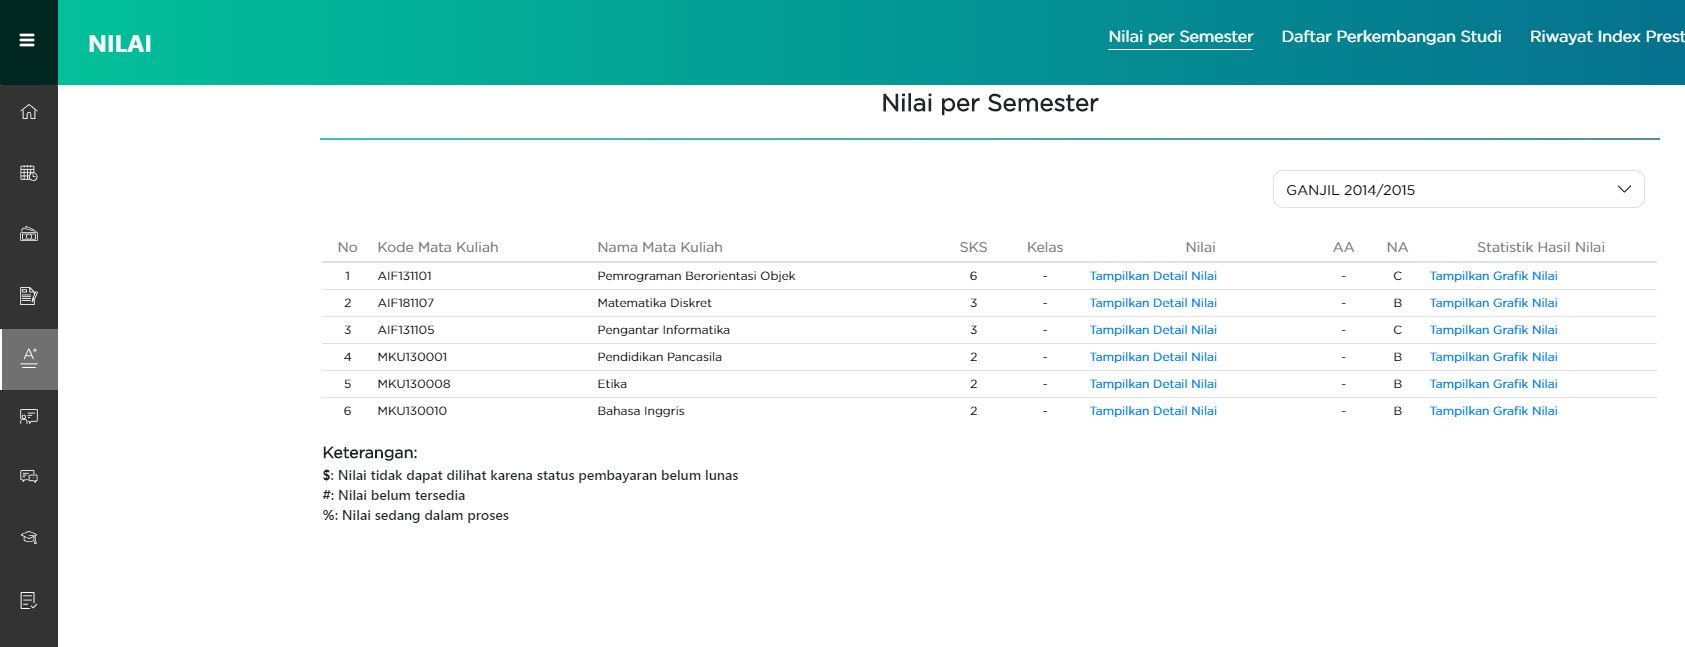
\includegraphics[scale=0.35]{Gambar/HasilPengujian/2014_2_nps_studentportal}
			\caption{Halaman Nilai Per Semester (Student Portal) - Elia}
			\label{fig:2014_2_nps_studentportal}
		\end{figure}
		\begin{figure}[H]
			\centering
			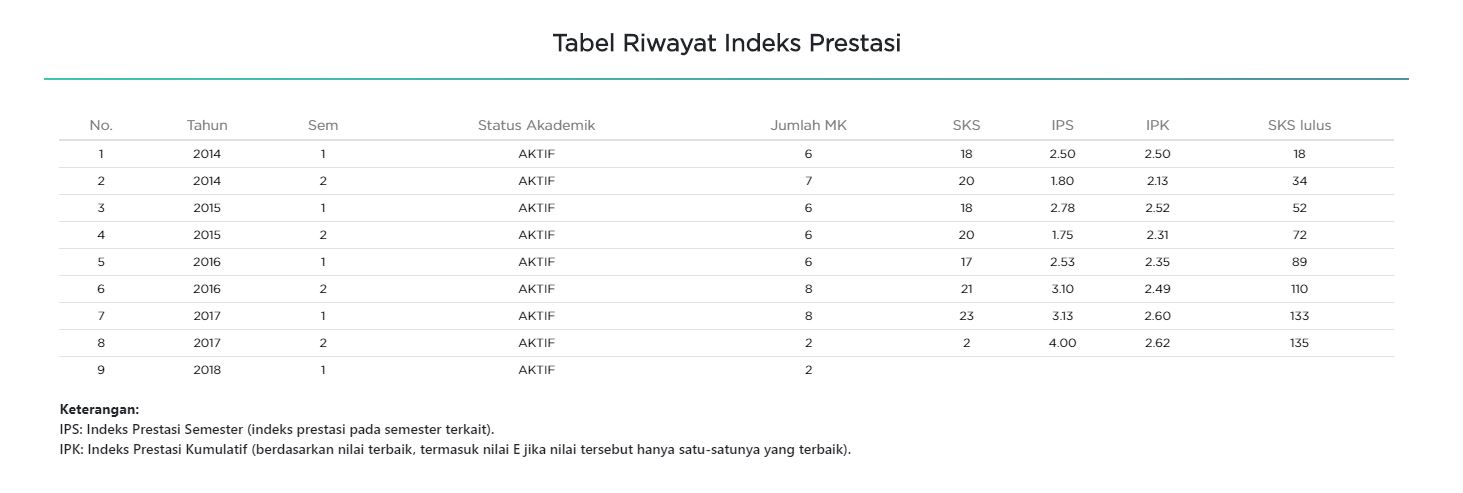
\includegraphics[scale=0.45]{Gambar/HasilPengujian/2014_2_rip_studentportal}
			\caption{Halaman Riwayat Indek Prestasi (Student Portal) - Elia}
			\label{fig:2014_2_rip_studentportal}
		\end{figure}
		\begin{figure}[H]
			\centering
			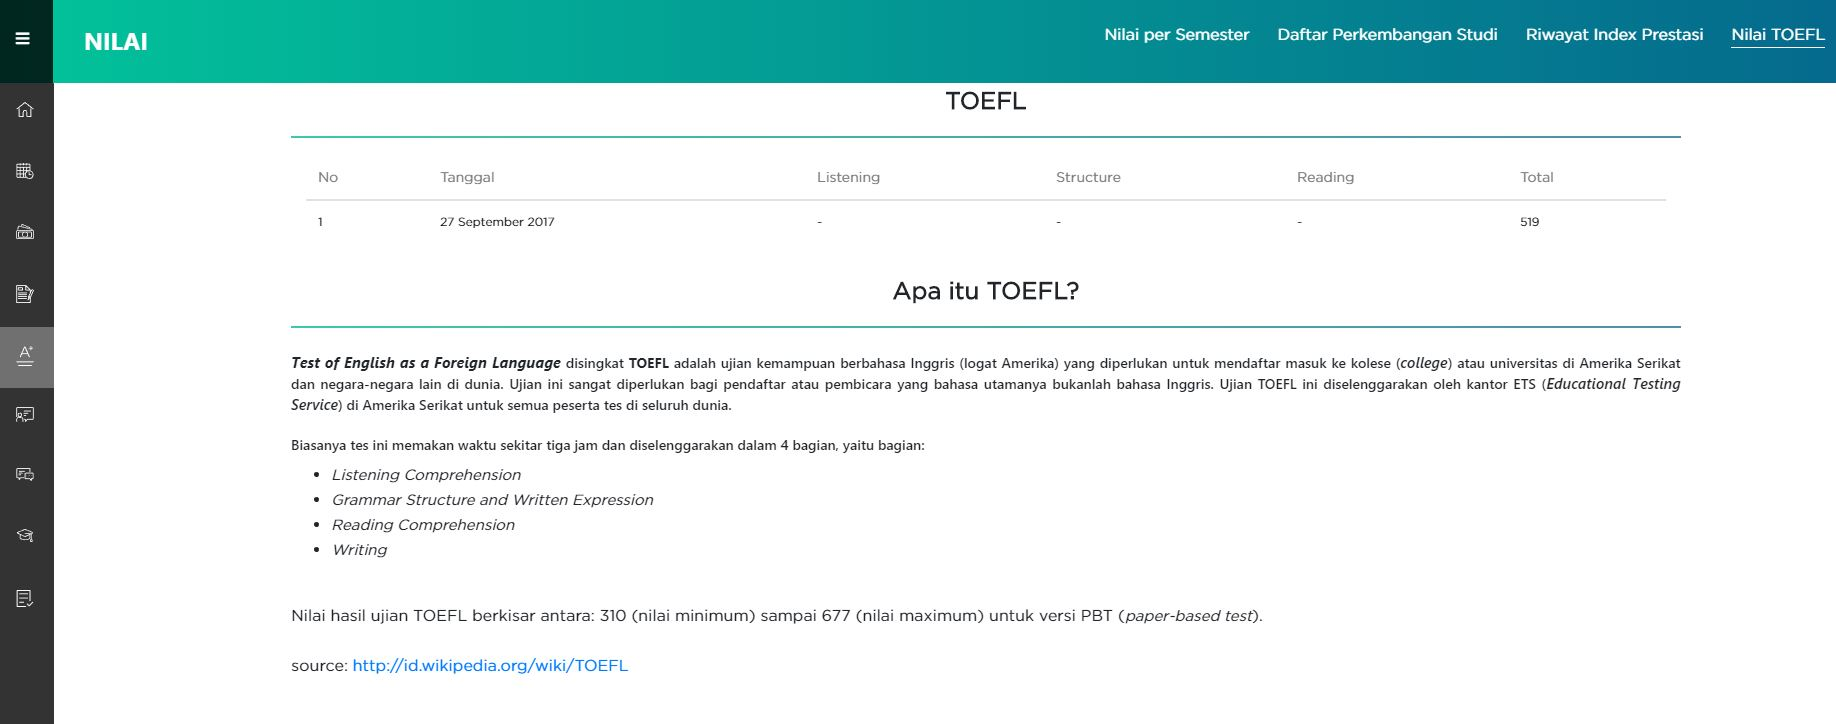
\includegraphics[scale=0.35]{Gambar/HasilPengujian/2014_2_toefl_studentportal}
			\caption{Halaman Nilai TOEFL (Student Portal) - Elia}
			\label{fig:2014_2_toefl_studentportal}
		\end{figure}
		\begin{figure}[H]
			\centering
			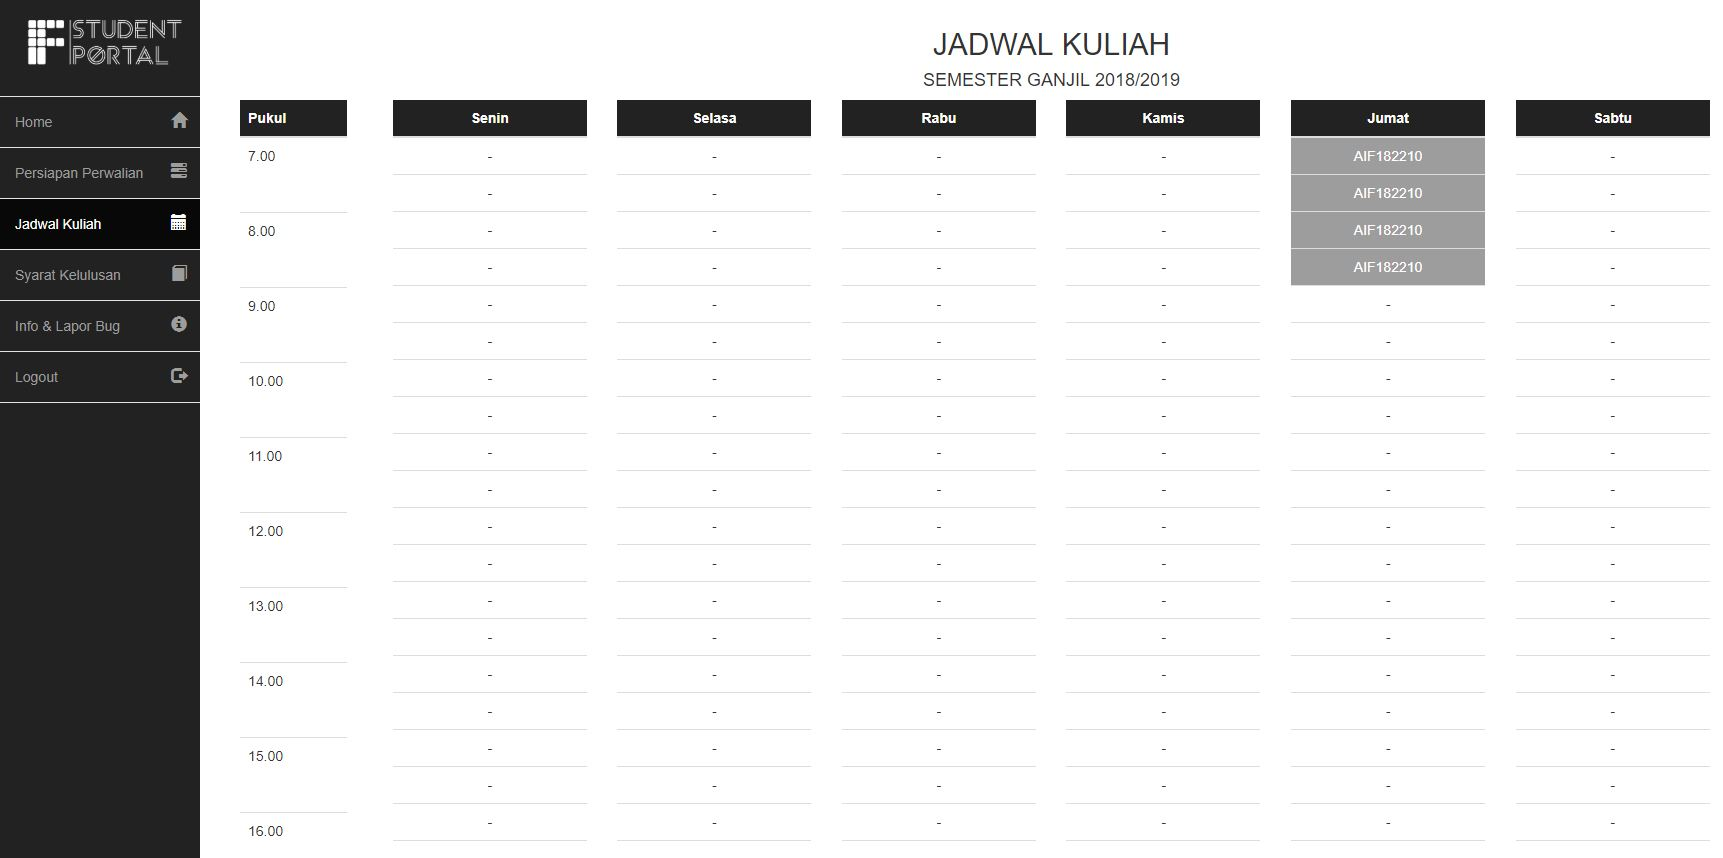
\includegraphics[scale=0.35]{Gambar/HasilPengujian/2014_2_jadwal_kuliah_ifstudentportal}
			\caption{Halaman Jadwal Kuliah (IFStudentPortal) - Elia}
			\label{fig:2014_2_jadwal_kuliah_ifstudentportal}
		\end{figure}
		\begin{figure}[H]
			\centering
			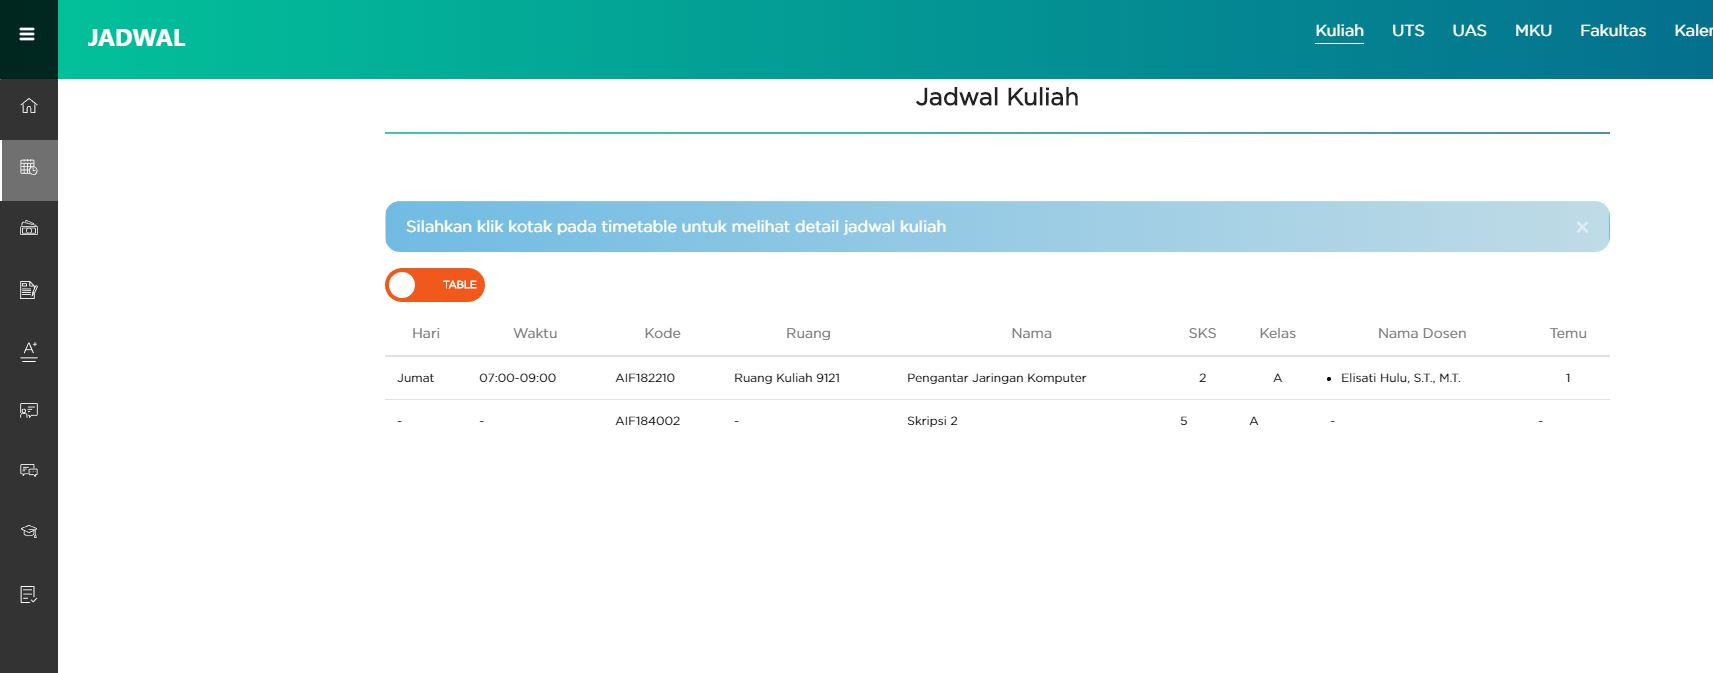
\includegraphics[scale=0.35]{Gambar/HasilPengujian/2014_2_jadwal_kuliah_studentportal}
			\caption{Halaman Jadwal Kuliah (Student Portal) - Elia}
			\label{fig:2014_2_jadwal_kuliah_studentportal}
		\end{figure}
		Hasil pengujian eksperimental halaman persiapan perwalian dari IFStudentPortal yang berisi data akademik (IPS, IPK, IP Lulus, IP Nilai Terbaik, sks lulus, dan nilai TOEFL) dan data mata kuliah berserta prasyaratnya dapat dilihat pada Gambar \ref{fig:2014_2_persiapan_perwalian_ifstudentportal}. Gambar \ref{fig:2014_2_rip_studentportal} menunjukkan riwayat IP sedangkan Gambar \ref{fig:2014_2_nps_studentportal} menunjukkan salah satu nilai per semester mahasiswa dan Gambar \ref{fig:2014_2_toefl_studentportal} menunjukkan riwayat nilai TOEFL mahasiswa. Hasil tersebut menunjukkan bahwa halaman persiapan perwalian sudah sesuai dengan data mahasiswa pada Student Portal. Hasil pengujian berikutnya mahasiswa melakukan pemeriksaan syarat kelulusan terdapat syarat yang seharusnya sudah lulus yaitu ``Anda belum mengambil salah satu dari MK Proyek AIF183106 atau AIF183308 \& AIF184303''(Gambar \ref{fig:2014_2_syarat_kelulusan_ifstudentportal}). Hal ini disebabkan perbedaan kode mata kuliah ``Proyek Sistem Infomasi 2'' dengan \cite{dokumenkurikulum2018}. Pada \cite{dokumenkurikulum2018} dituliskan hasil transisi untuk mata kuliah ``Proyek Sistem Infomasi 2'' adalah ``AIF184303'', sedangkan pada StudentPortal adalah ``AIF134405''(Gambar \ref{fig:2014_2_nps_studentportal}). Hasil pengujian berikutnya dapat dilihat pada Gambar \ref{fig:2014_2_jadwal_kuliah_ifstudentportal} menunjukan jadwal kuliah mahasiswa pada IFStudentPortal. Kemudian jadwal kuliah mahasiswa pada Student Portal dapat dilihat pada Gambar \ref{fig:2014_2_jadwal_kuliah_studentportal}. Hasil tersebut menunjukkan bahwa jadwal kuliah dari IFStudentPortal sudah sesuai dengan jadwal kuliah pada Student Portal.
	\end{enumerate}
	Hasil pengujian eksperimental pada mahasiswa Fedrian Hermana sesuai dengan hasil yang diharapkan, tetapi pada mahasiswa Elia terdapat hasil belum sesuai dengan yang diharapkan.
	\item Angkatan 2015 \\
	Untuk angkatan 2015 pengujian dilakukan kepada dua orang mahasiswa, yaitu:
	\begin{enumerate}
		\item Ebenhaezer Hardani - 2015730015
		\begin{figure}[H]
			\centering
			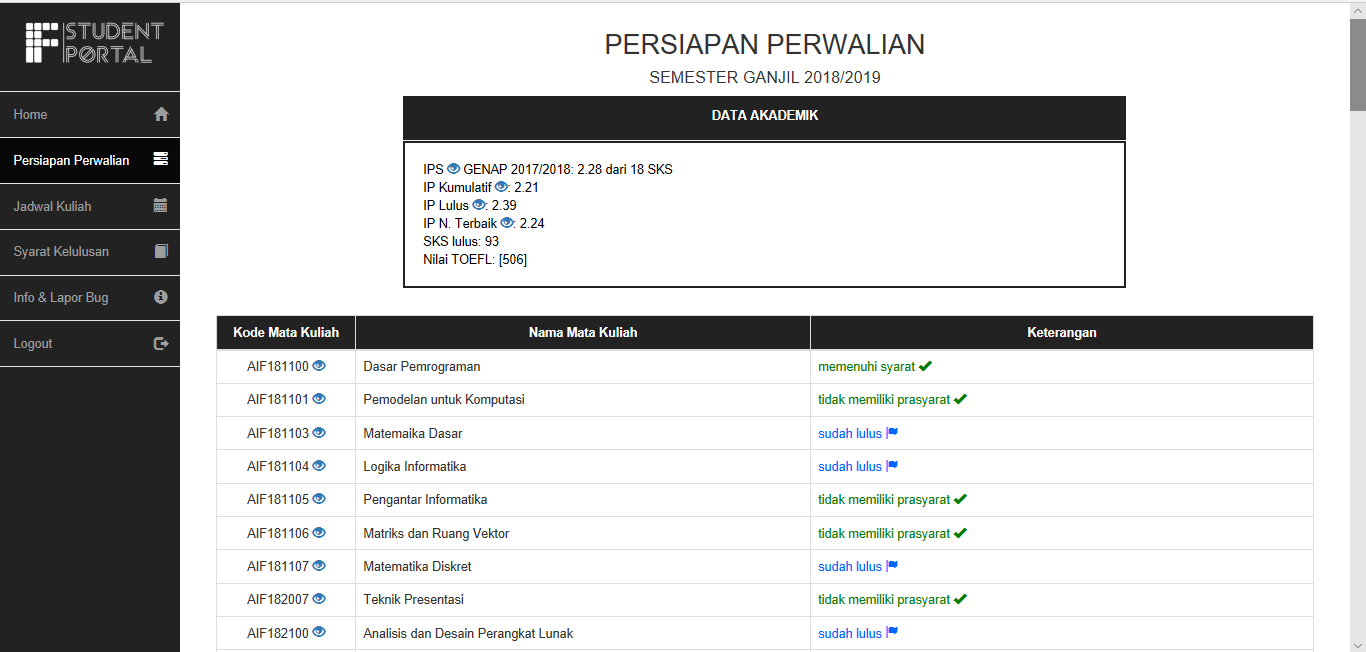
\includegraphics[scale=0.45]{Gambar/HasilPengujian/2015_1_persiapan_perwalian_ifstudentportal}
			\caption{Halaman Persiapan Perwalian (IFStudentPortal) - Ebenhaezer Hardani}
			\label{fig:2015_1_persiapan_perwalian_ifstudentportal}
		\end{figure}
		\begin{figure}[H]
			\centering
			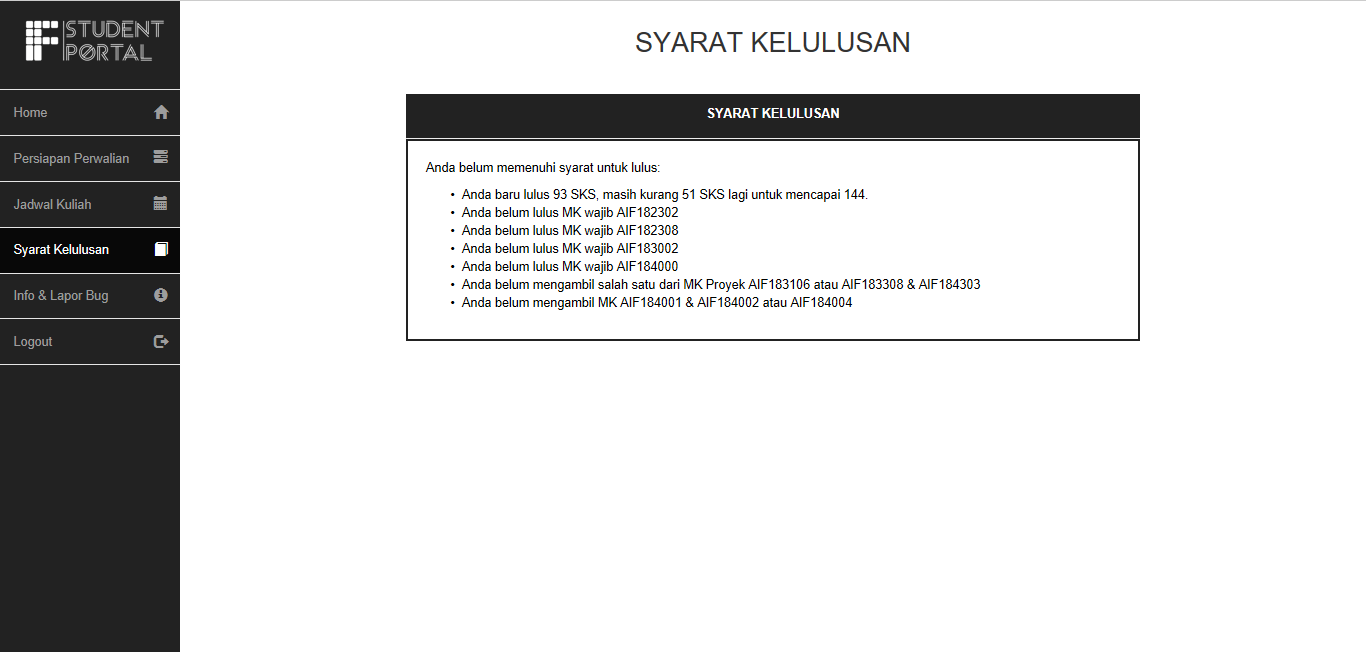
\includegraphics[scale=0.45]{Gambar/HasilPengujian/2015_1_syarat_kelulusan_ifstudentportal}
			\caption{Halaman Syarat Kelulusan (IFStudentPortal) - Ebenhaezer Hardani}
			\label{fig:2015_1_syarat_kelulusan_ifstudentportal}
		\end{figure}
		\begin{figure}[H]
			\centering
			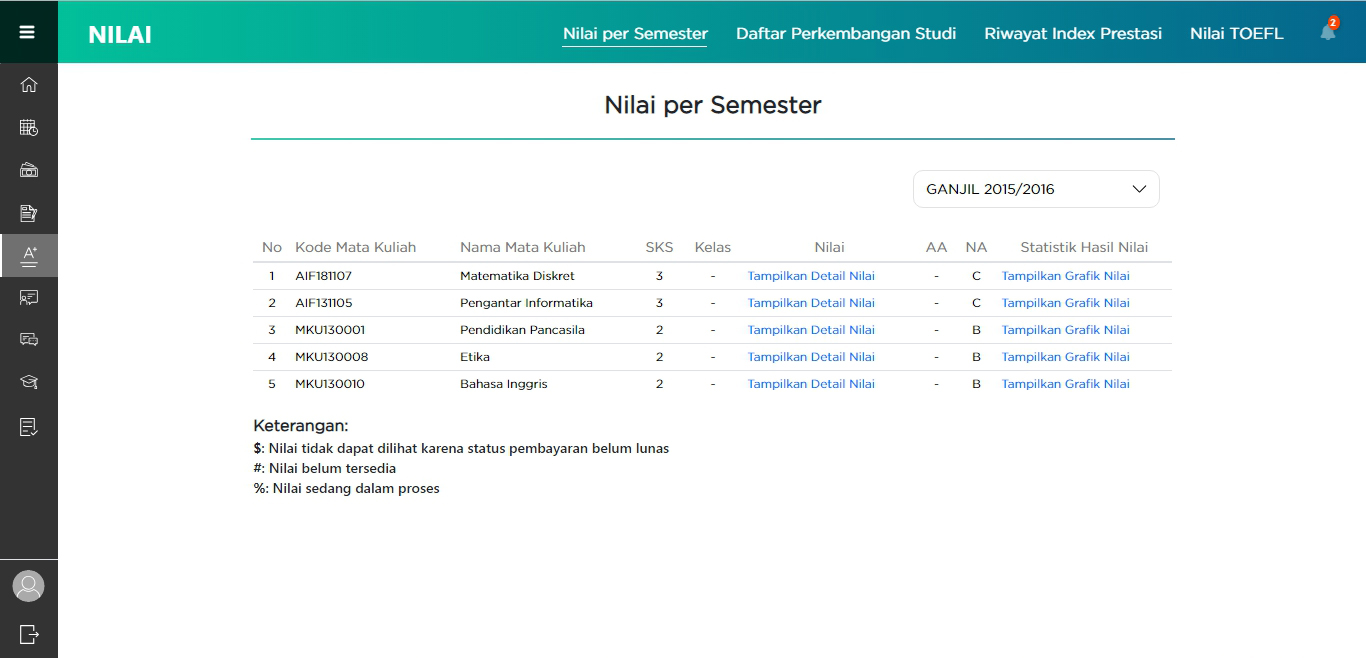
\includegraphics[scale=0.45]{Gambar/HasilPengujian/2015_1_nps_studentportal}
			\caption{Halaman Nilai Per Semester (Student Portal) - Ebenhaezer Hardani}
			\label{fig:2015_1_nps_studentportal}
		\end{figure}
		\begin{figure}[H]
			\centering
			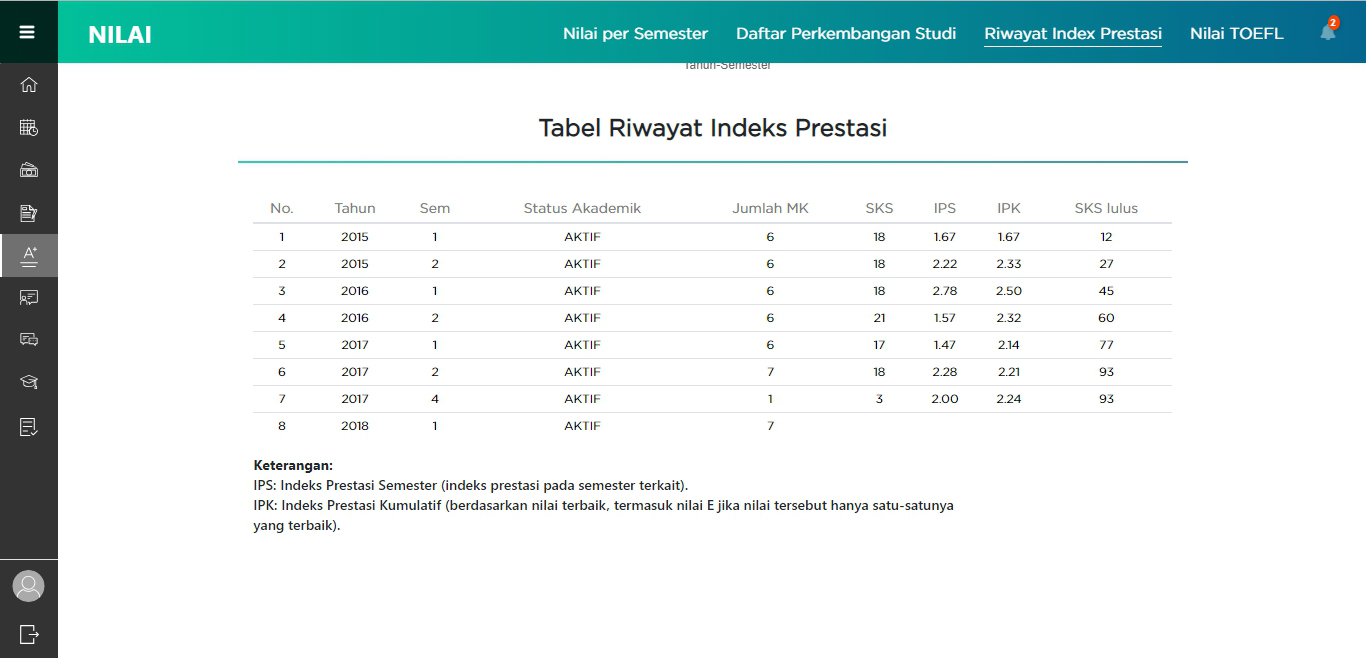
\includegraphics[scale=0.45]{Gambar/HasilPengujian/2015_1_rip_studentportal}
			\caption{Halaman Riwayat Indek Prestasi (Student Portal) - Ebenhaezer Hardani}
			\label{fig:2015_1_rip_studentportal}
		\end{figure}
		\begin{figure}[H]
			\centering
			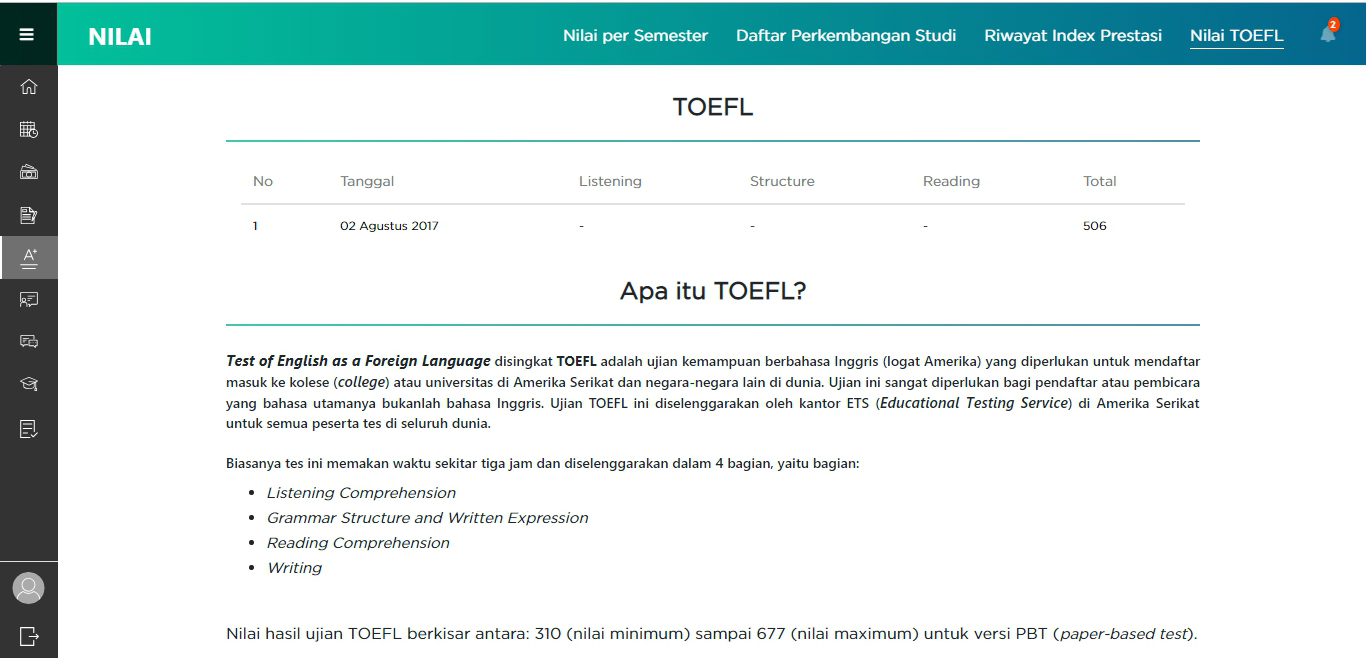
\includegraphics[scale=0.45]{Gambar/HasilPengujian/2015_1_toefl_studentportal}
			\caption{Halaman Nilai TOEFL (Student Portal) - Ebenhaezer Hardani}
			\label{fig:2015_1_toefl_studentportal}
		\end{figure}
		\begin{figure}[H]
			\centering
			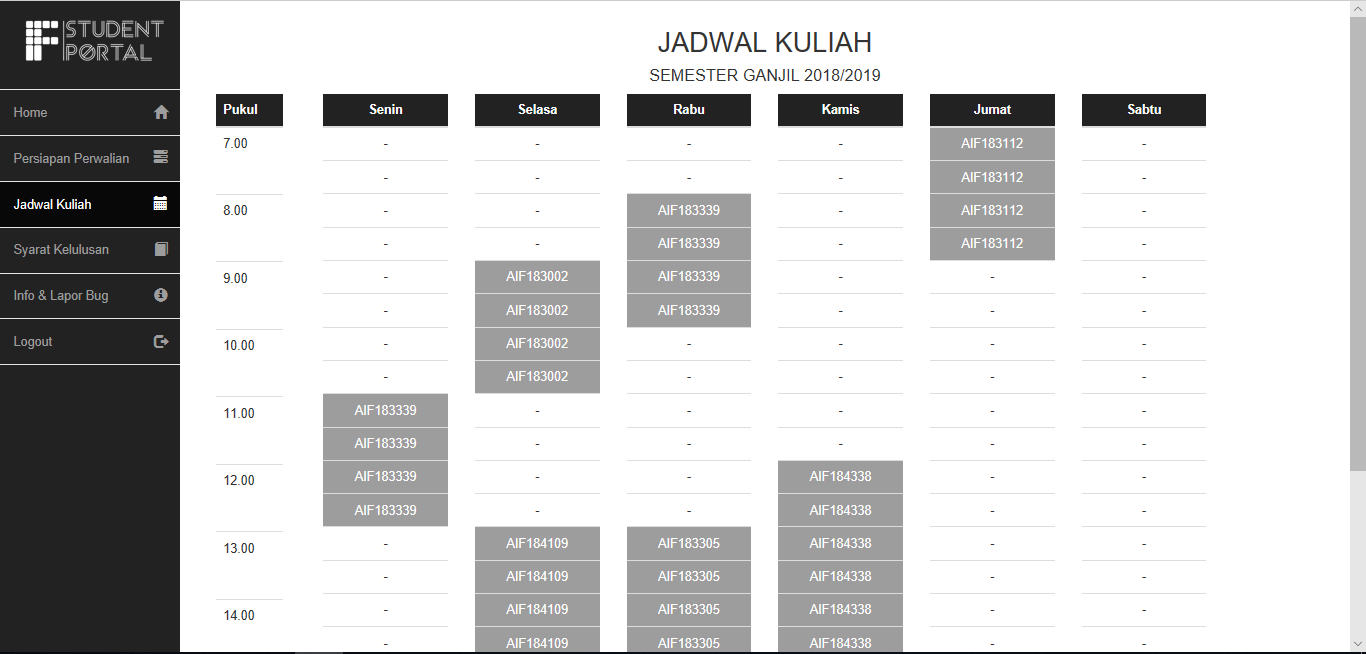
\includegraphics[scale=0.45]{Gambar/HasilPengujian/2015_1_jadwal_kuliah_ifstudentportal}
			\caption{Halaman Jadwal Kuliah (IFStudentPortal) - Ebenhaezer Hardani}
			\label{fig:2015_1_jadwal_kuliah_ifstudentportal}
		\end{figure}
		\begin{figure}[H]
			\centering
			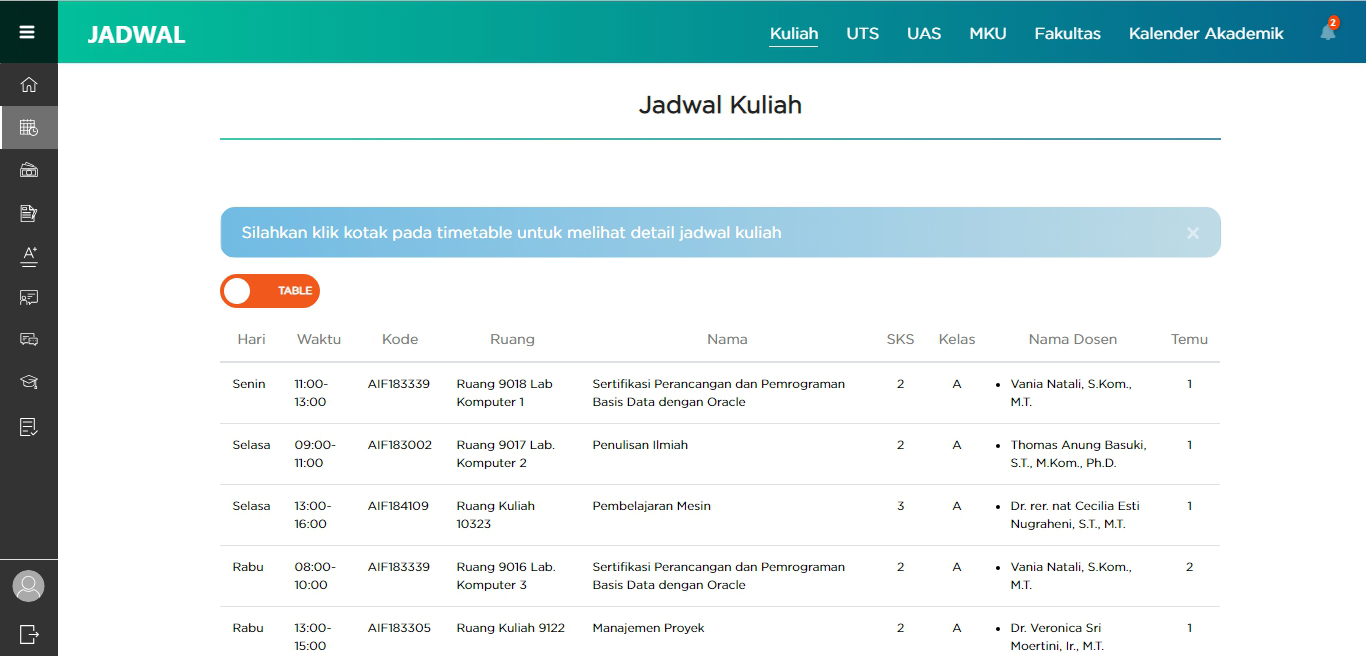
\includegraphics[scale=0.45]{Gambar/HasilPengujian/2015_1_jadwal_kuliah_studentportal}
			\caption{Halaman Jadwal Kuliah (Student Portal) - Ebenhaezer Hardani}
			\label{fig:2015_1_jadwal_kuliah_studentportal}
		\end{figure}
		Hasil pengujian eksperimental halaman persiapan perwalian dari IFStudentPortal yang berisi data akademik (IPS, IPK, IP Lulus, IP Nilai Terbaik, sks lulus, dan nilai TOEFL) dan data mata kuliah berserta prasyaratnya dapat dilihat pada Gambar \ref{fig:2015_1_persiapan_perwalian_ifstudentportal}. Gambar \ref{fig:2015_1_rip_studentportal} menunjukkan riwayat IP sedangkan Gambar \ref{fig:2015_1_nps_studentportal} menunjukkan salah satu nilai per semester mahasiswa dan Gambar \ref{fig:2015_1_toefl_studentportal} menunjukkan riwayat nilai TOEFL mahasiswa. Hasil tersebut menunjukkan bahwa halaman persiapan perwalian sudah sesuai dengan data mahasiswa pada Student Portal. Hasil pengujian berikutnya dapat dilihat pada Gambar \ref{fig:2015_1_syarat_kelulusan_ifstudentportal} menujukkan syarat lulus mahasiswa Teknik Informatika UNPAR sedangkan Gambar \ref{fig:2015_1_nps_studentportal} menujukkan salah satu data nilai hasil transisi ke kurikulum 2018. Hasil tersebut menunjukkan bahwa halaman syarat kelulusan telah sesuai dengan hasil yang diharapkan. Hasil pengujian berikutnya dapat dilihat pada Gambar \ref{fig:2015_1_jadwal_kuliah_ifstudentportal} menunjukan jadwal kuliah mahasiswa pada IFStudentPortal. Kemudian jadwal kuliah mahasiswa pada Student Portal dapat dilihat pada Gambar \ref{fig:2015_1_jadwal_kuliah_studentportal}. Hasil tersebut menunjukkan bahwa jadwal kuliah dari IFStudentPortal sudah sesuai dengan jadwal kuliah pada Student Portal.
		\item Hizkia Steven - 2015730020
		\begin{figure}[H]
			\centering
			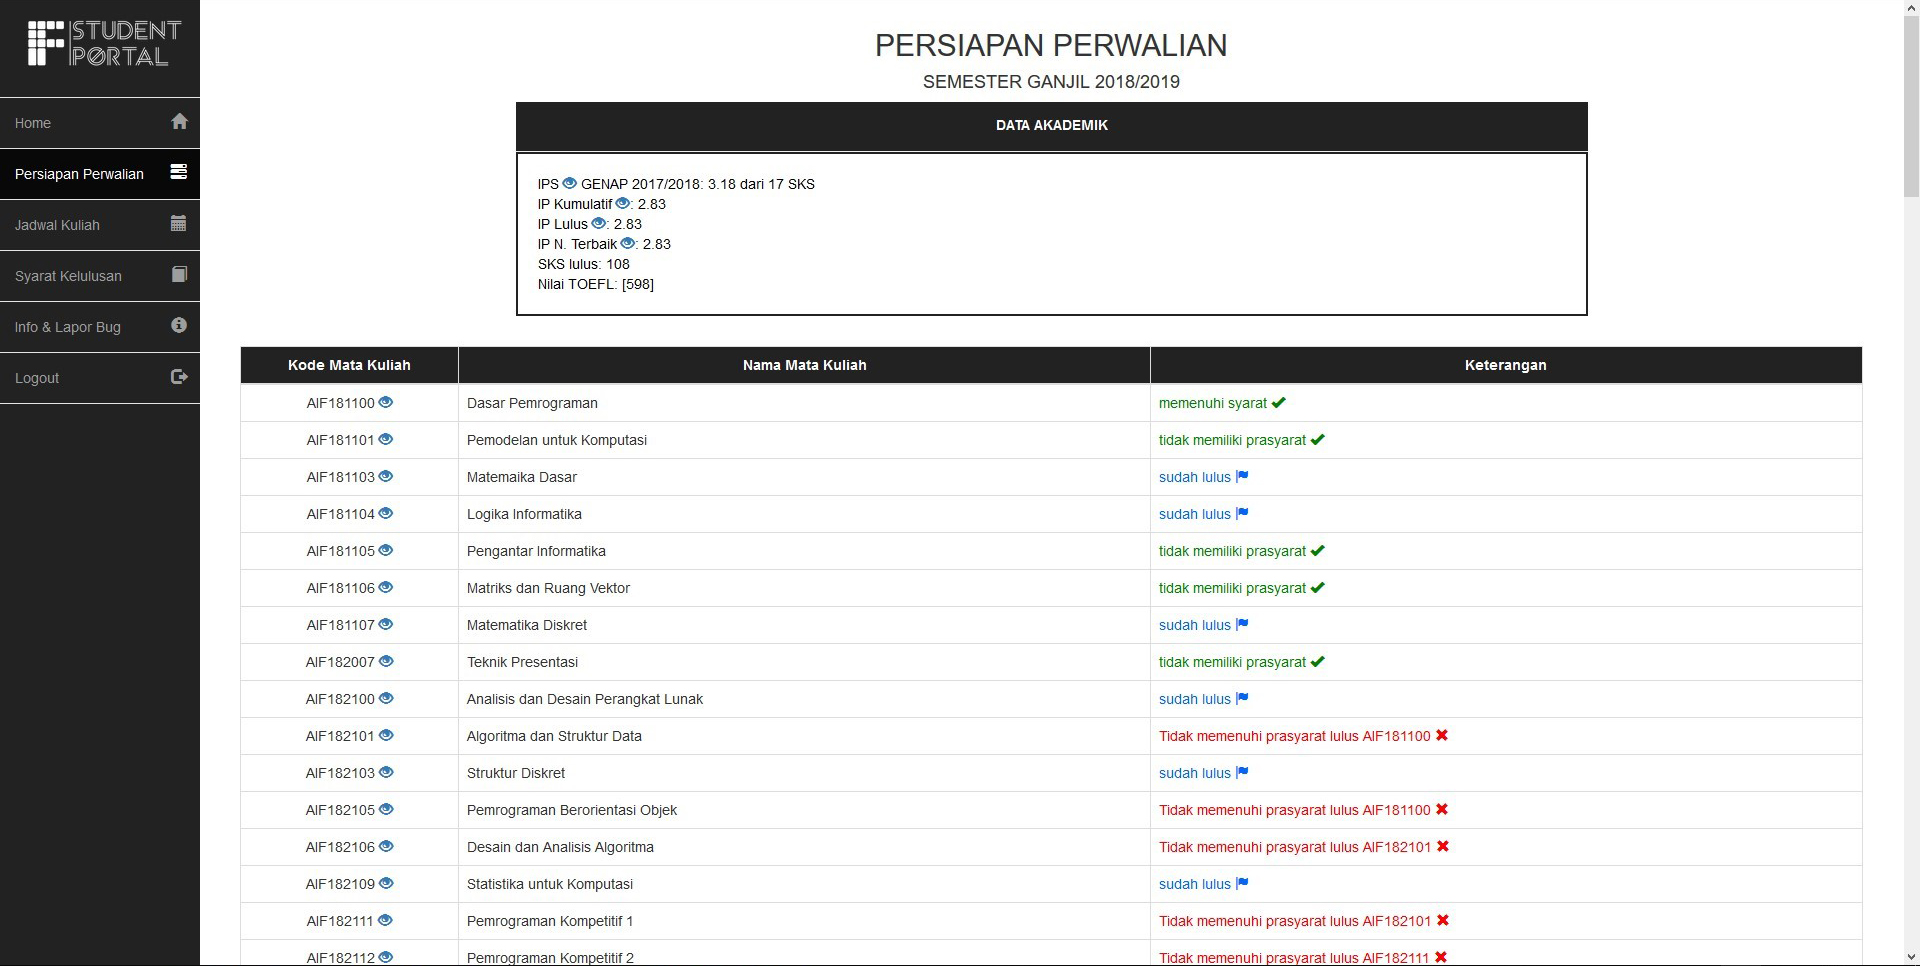
\includegraphics[scale=0.325]{Gambar/HasilPengujian/2015_2_persiapan_perwalian_ifstudentportal}
			\caption{Halaman Persiapan Perwalian (IFStudentPortal) - Hizkia Steven}
			\label{fig:2015_2_persiapan_perwalian_ifstudentportal}
		\end{figure}
		\begin{figure}[H]
			\centering
			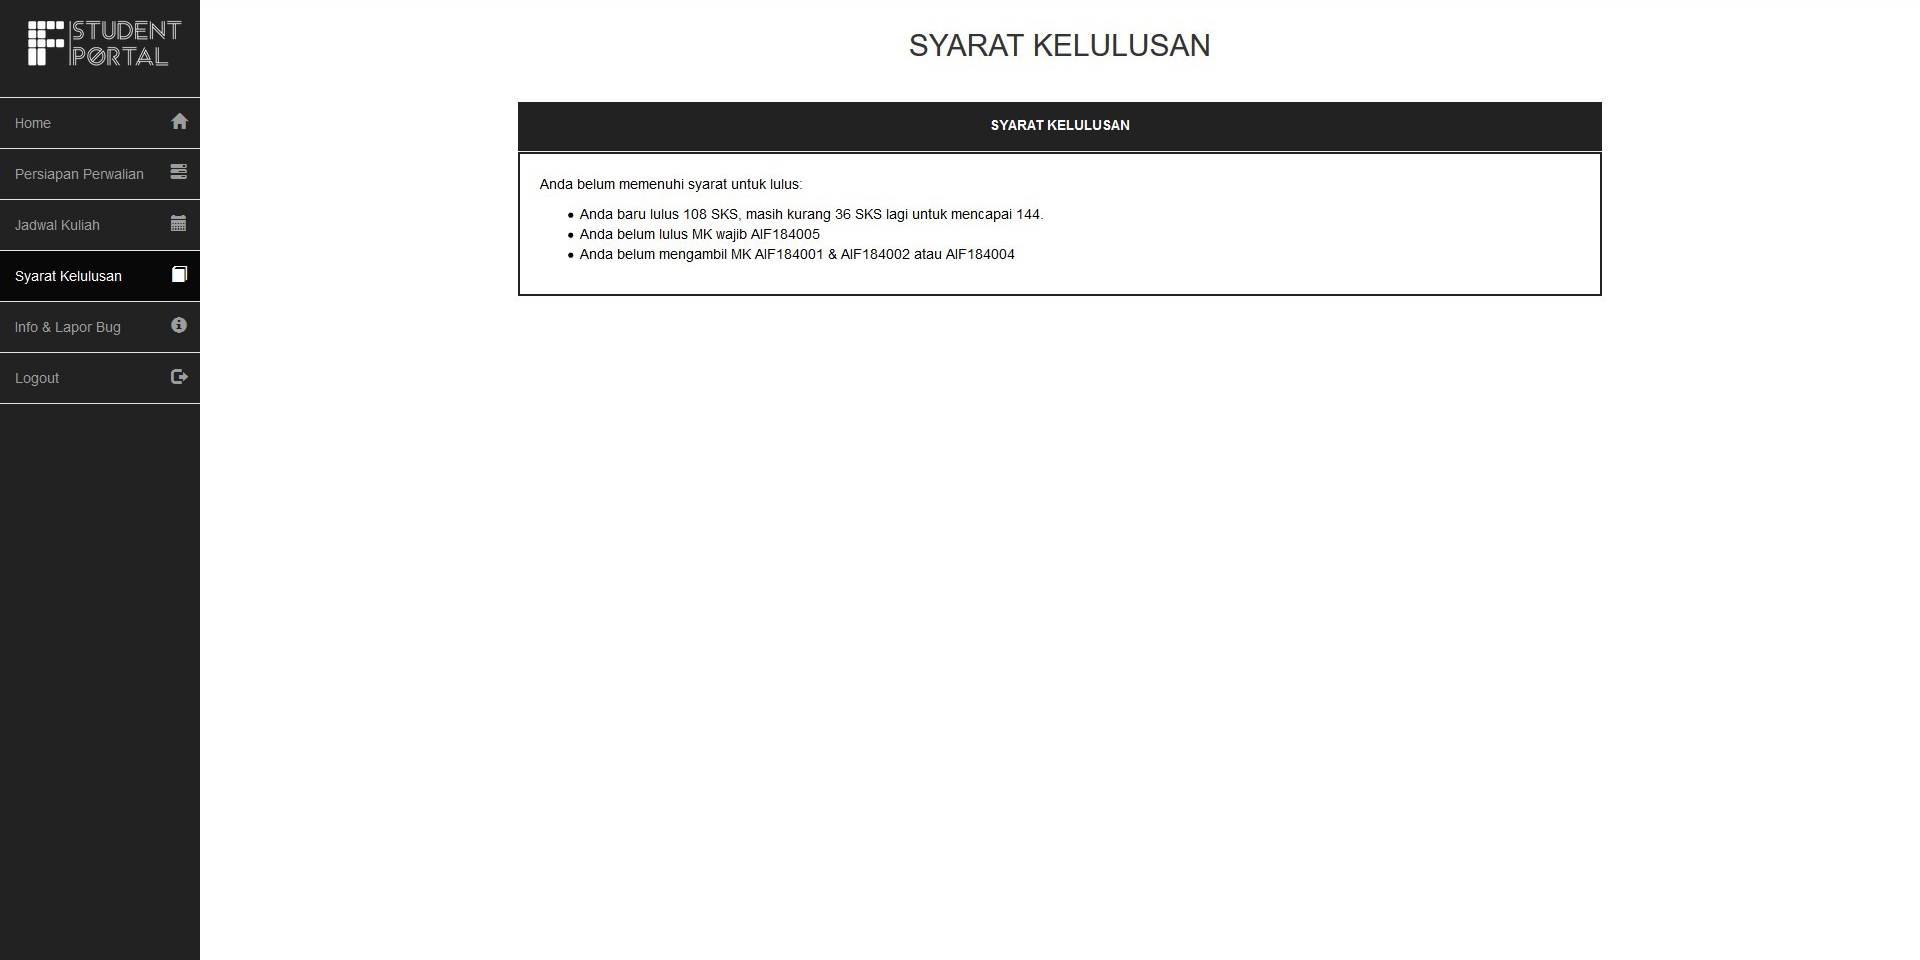
\includegraphics[scale=0.325]{Gambar/HasilPengujian/2015_2_syarat_kelulusan_ifstudentportal}
			\caption{Halaman Syarat Kelulusan (IFStudentPortal) - Hizkia Steven}
			\label{fig:2015_2_syarat_kelulusan_ifstudentportal}
		\end{figure}
		\begin{figure}[H]
			\centering
			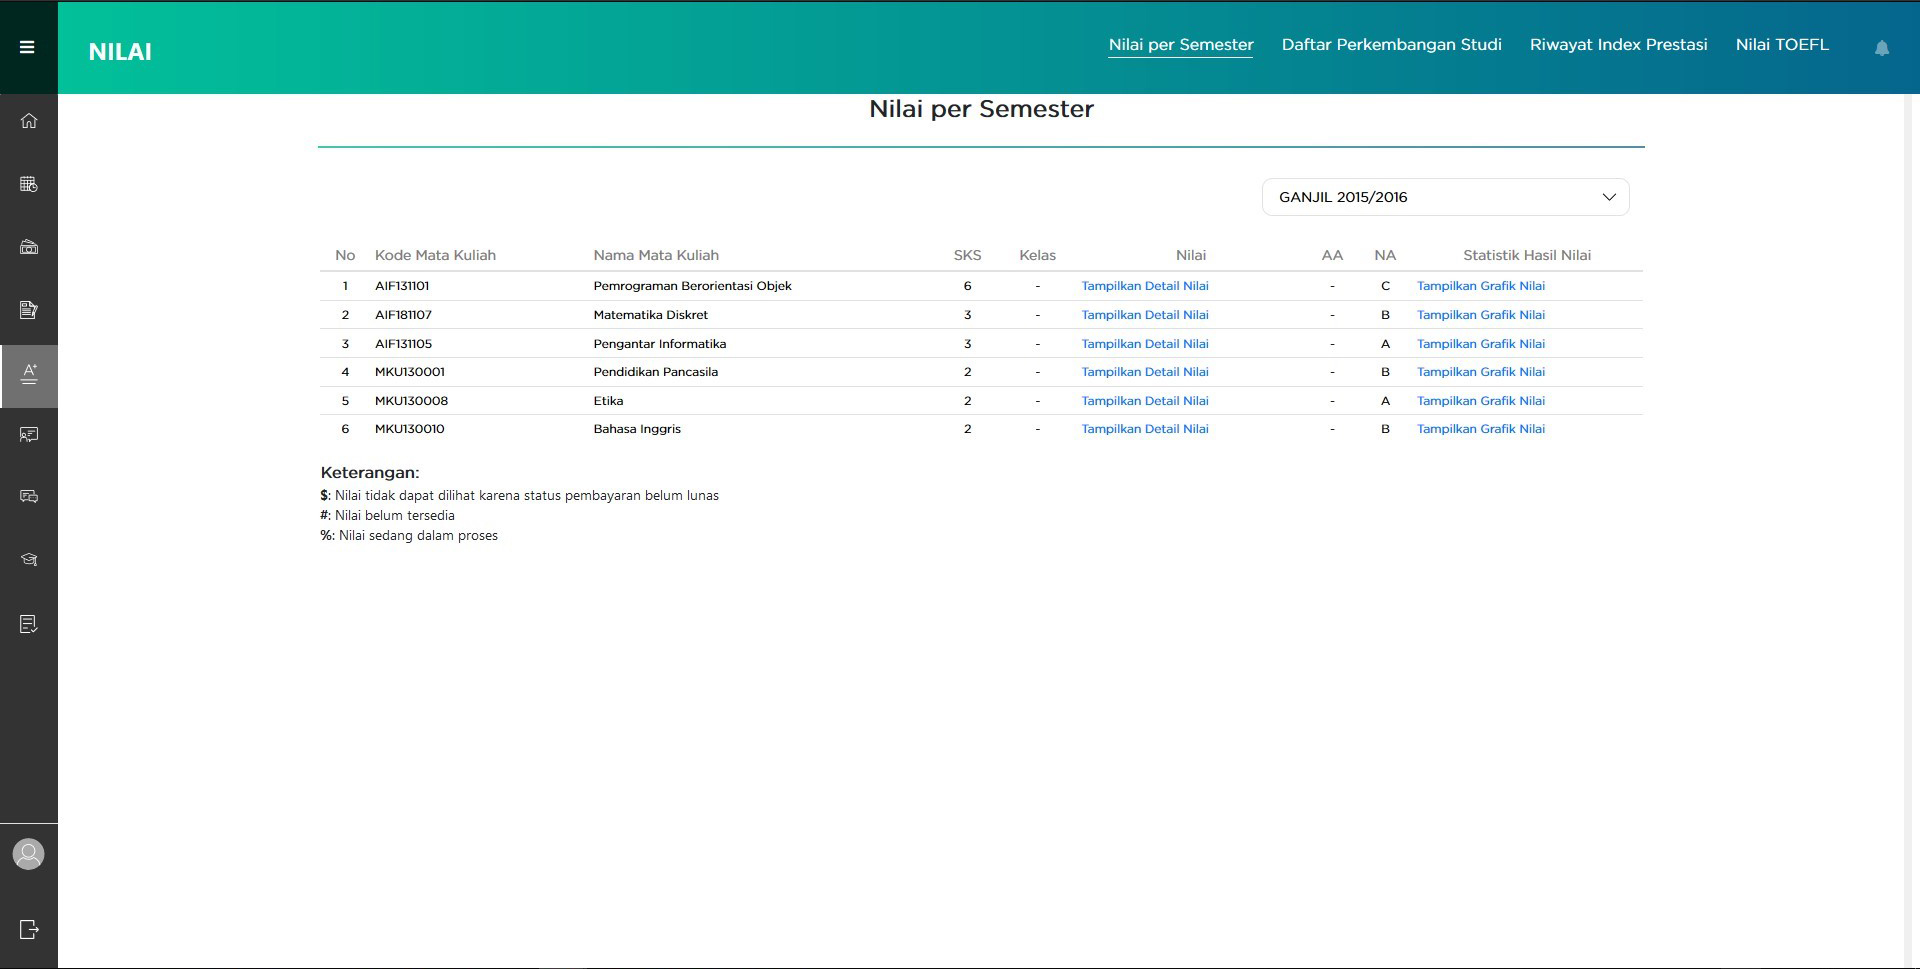
\includegraphics[scale=0.325]{Gambar/HasilPengujian/2015_2_nps_studentportal}
			\caption{Halaman Nilai Per Semester (Student Portal) - Hizkia Steven}
			\label{fig:2015_2_nps_studentportal}
		\end{figure}
		\begin{figure}[H]
			\centering
			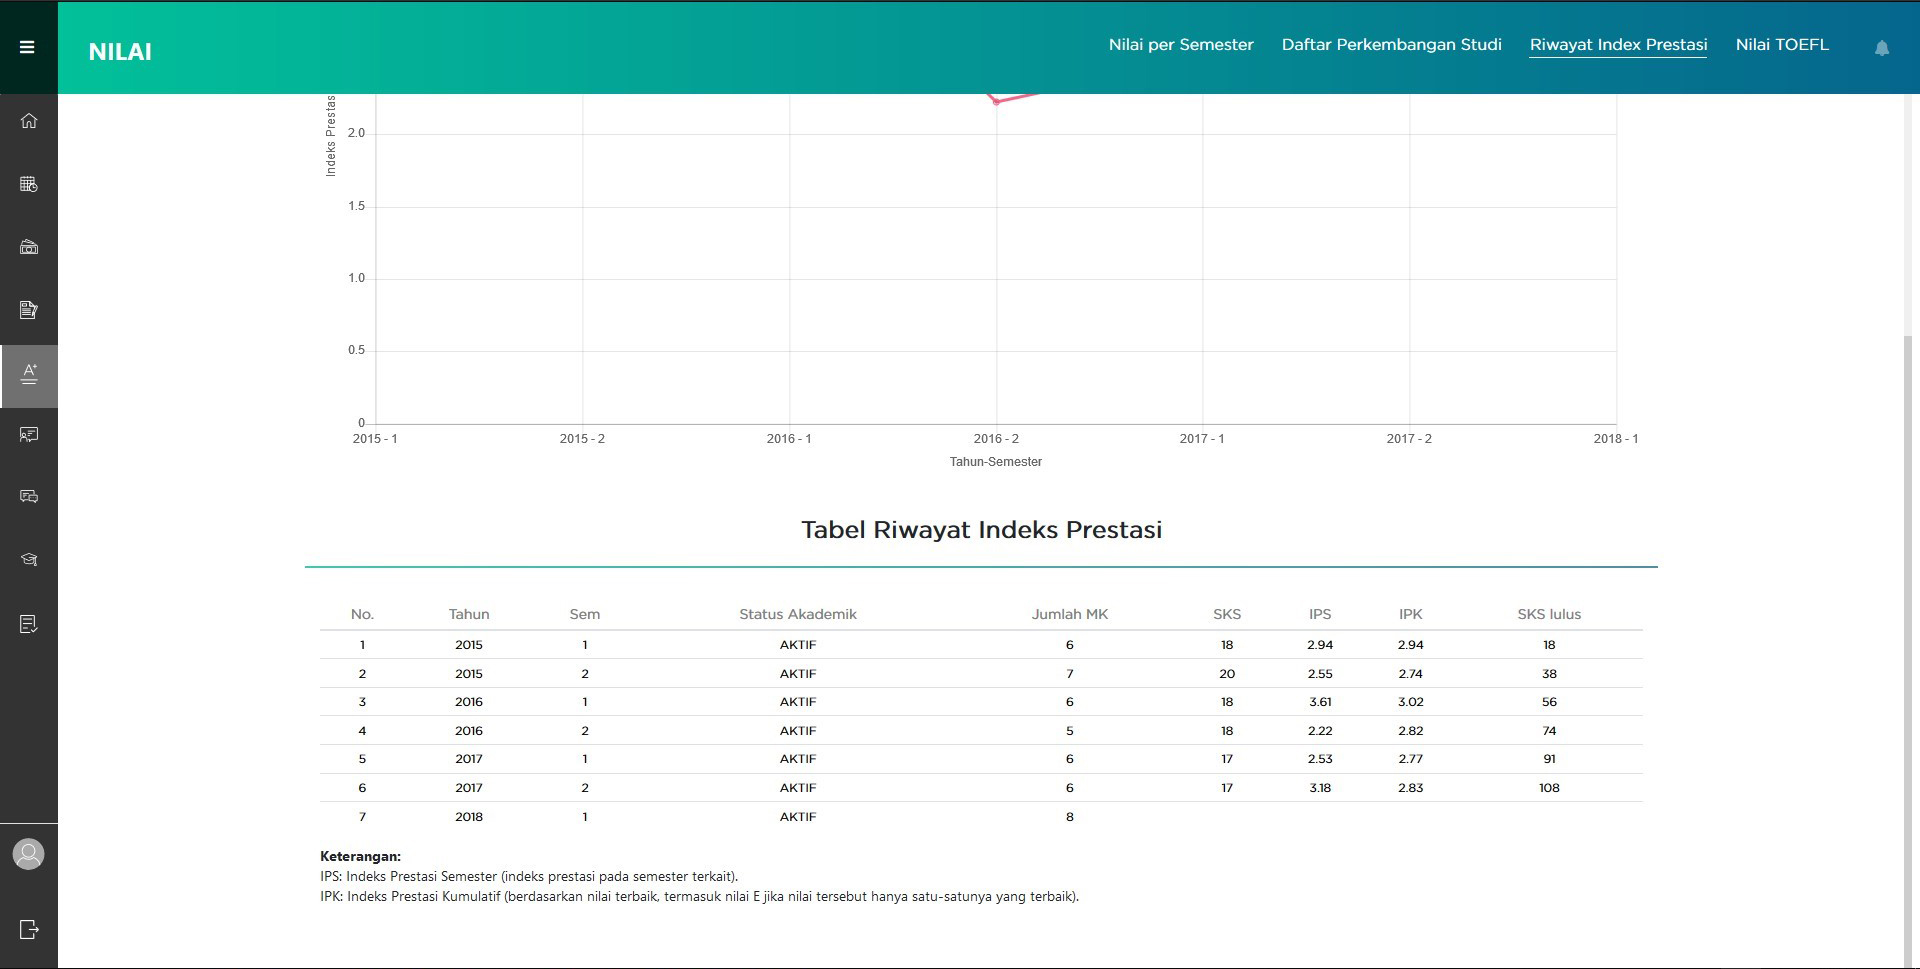
\includegraphics[scale=0.325]{Gambar/HasilPengujian/2015_2_rip_studentportal}
			\caption{Halaman Riwayat Indek Prestasi (Student Portal) - Hizkia Steven}
			\label{fig:2015_2_rip_studentportal}
		\end{figure}
		\begin{figure}[H]
			\centering
			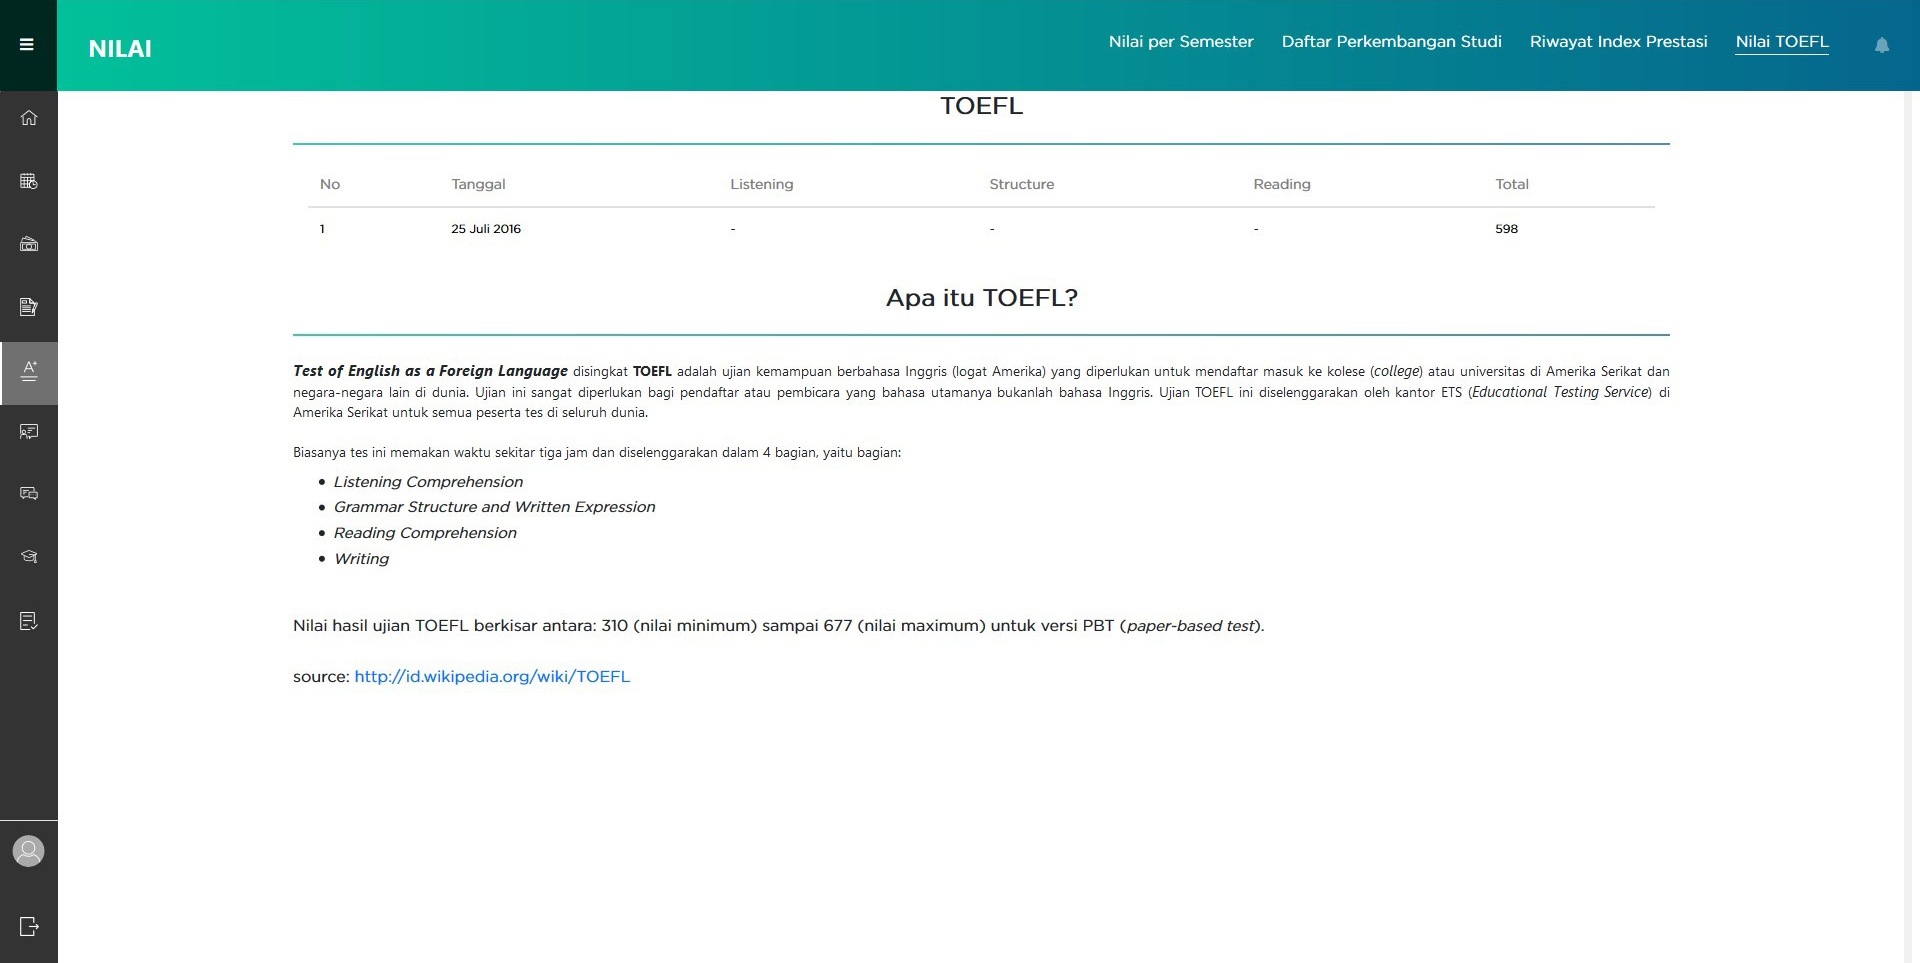
\includegraphics[scale=0.325]{Gambar/HasilPengujian/2015_2_toefl_studentportal}
			\caption{Halaman Nilai TOEFL (Student Portal) - Hizkia Steven}
			\label{fig:2015_2_toefl_studentportal}
		\end{figure}
		\begin{figure}[H]
			\centering
			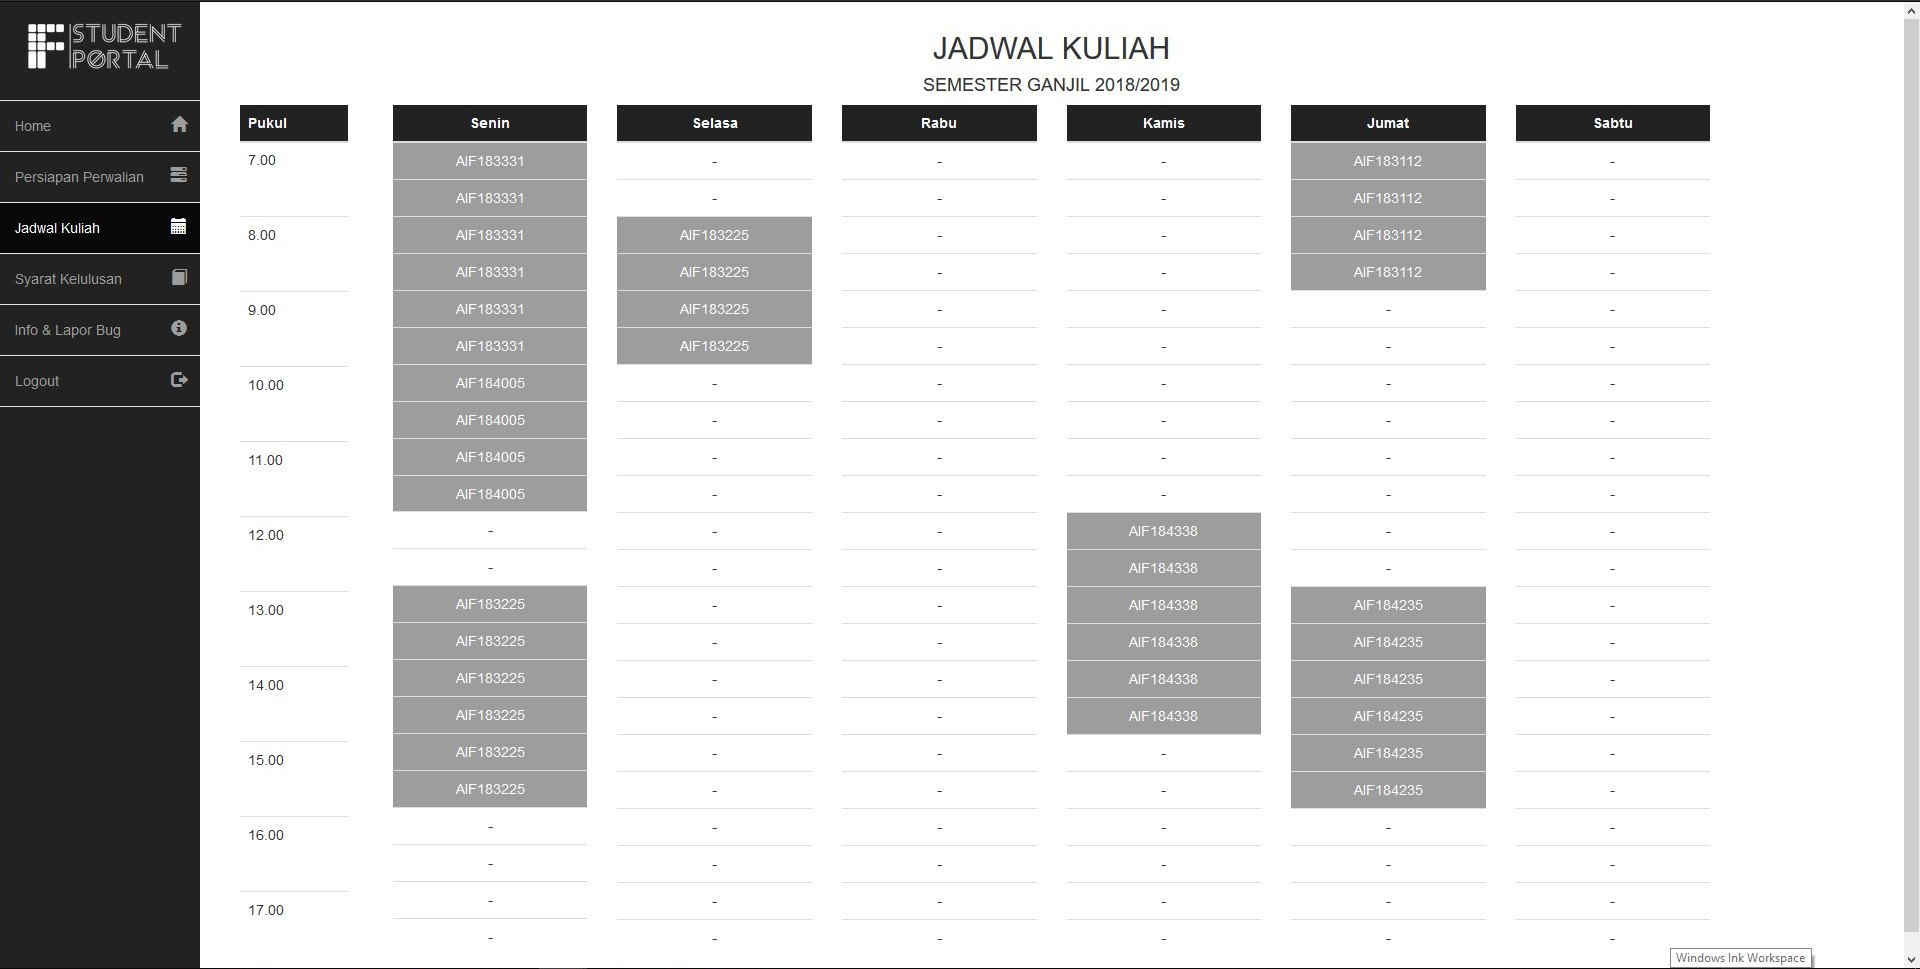
\includegraphics[scale=0.325]{Gambar/HasilPengujian/2015_2_jadwal_kuliah_ifstudentportal}
			\caption{Halaman Jadwal Kuliah (IFStudentPortal) - Hizkia Steven}
			\label{fig:2015_2_jadwal_kuliah_ifstudentportal}
		\end{figure}
		\begin{figure}[H]
			\centering
			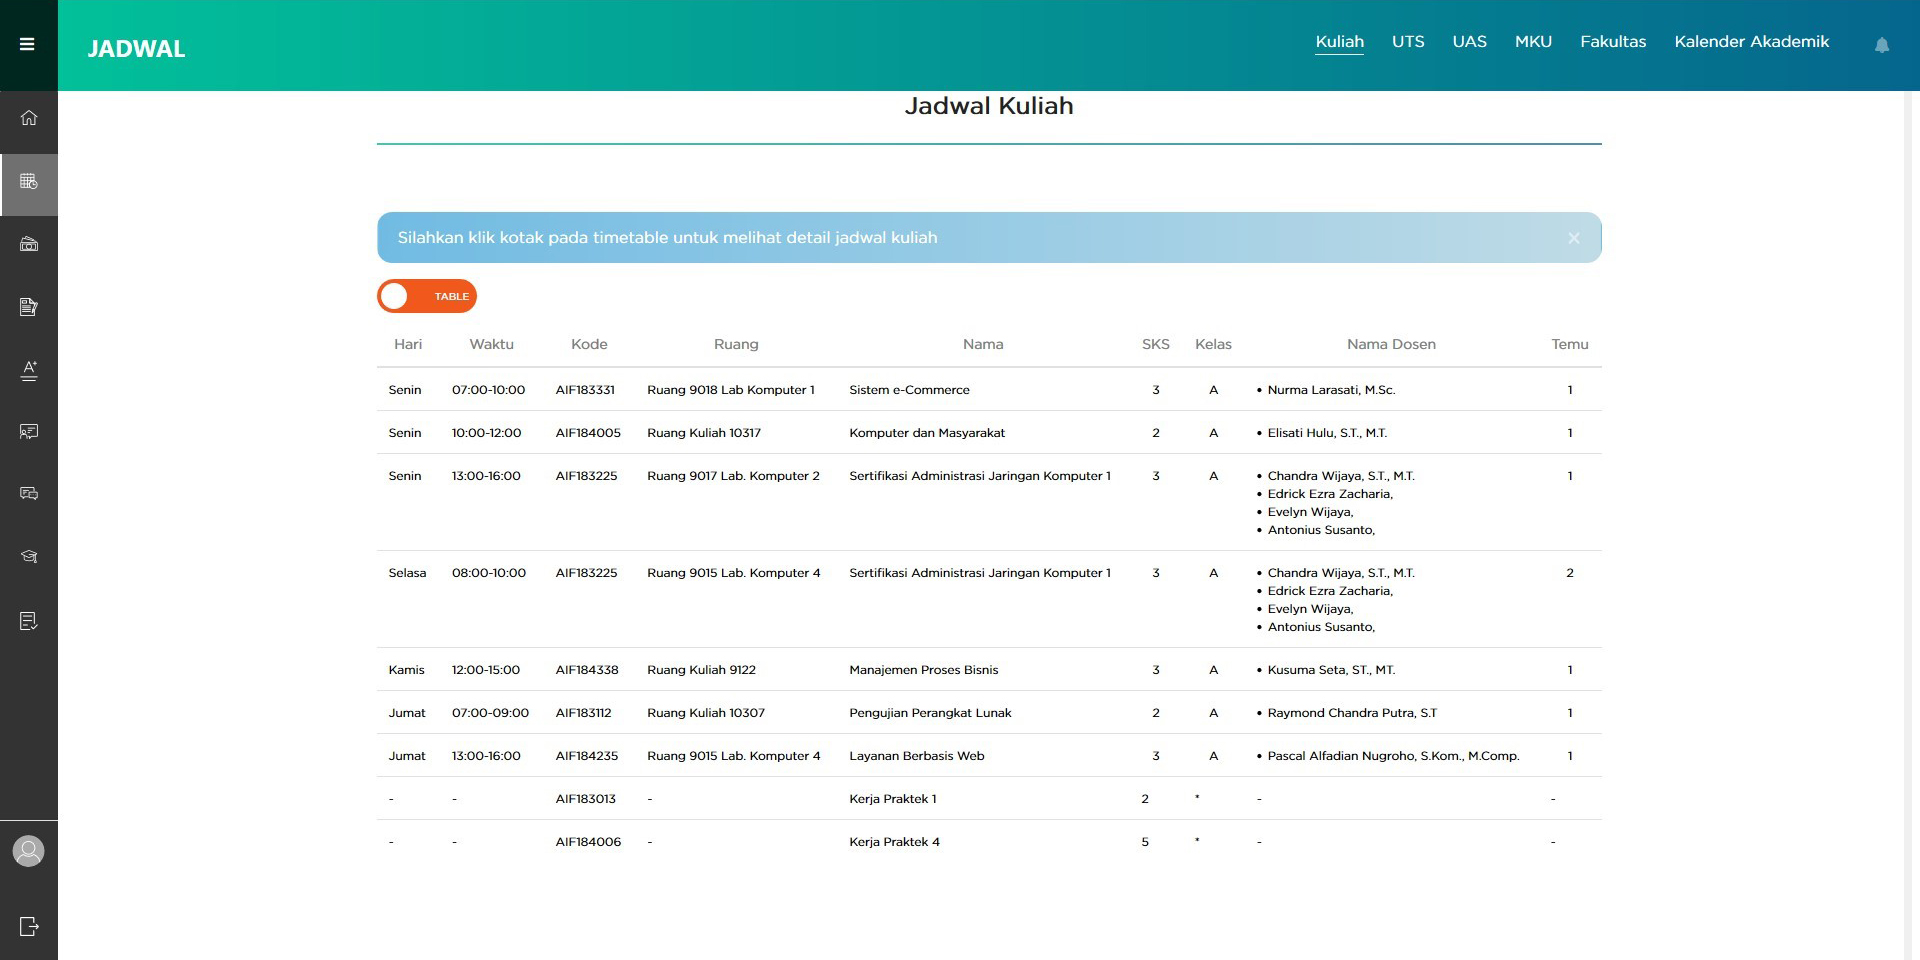
\includegraphics[scale=0.3]{Gambar/HasilPengujian/2015_2_jadwal_kuliah_studentportal}
			\caption{Halaman Jadwal Kuliah (Student Portal) - Hizkia Steven}
			\label{fig:2015_2_jadwal_kuliah_studentportal}
		\end{figure}
		Hasil pengujian eksperimental halaman persiapan perwalian dari IFStudentPortal yang berisi data akademik (IPS, IPK, IP Lulus, IP Nilai Terbaik, sks lulus, dan nilai TOEFL) dan data mata kuliah berserta prasyaratnya dapat dilihat pada Gambar \ref{fig:2015_2_persiapan_perwalian_ifstudentportal}. Gambar \ref{fig:2015_2_rip_studentportal} menunjukkan riwayat IP sedangkan Gambar \ref{fig:2015_2_nps_studentportal} menunjukkan salah satu nilai per semester mahasiswa dan Gambar \ref{fig:2015_2_toefl_studentportal} menunjukkan riwayat nilai TOEFL mahasiswa. Hasil tersebut menunjukkan bahwa halaman persiapan perwalian sudah sesuai dengan data mahasiswa pada Student Portal. Hasil pengujian berikutnya dapat dilihat pada Gambar \ref{fig:2015_2_syarat_kelulusan_ifstudentportal} menujukkan syarat lulus mahasiswa Teknik Informatika UNPAR sedangkan Gambar \ref{fig:2015_2_nps_studentportal} menujukkan salah satu data nilai hasil transisi ke kurikulum 2018. Hasil tersebut menunjukkan bahwa halaman syarat kelulusan telah sesuai dengan hasil yang diharapkan. Hasil pengujian berikutnya dapat dilihat pada Gambar \ref{fig:2015_2_jadwal_kuliah_ifstudentportal} menunjukan jadwal kuliah mahasiswa pada IFStudentPortal. Kemudian jadwal kuliah mahasiswa pada Student Portal dapat dilihat pada Gambar \ref{fig:2015_2_jadwal_kuliah_studentportal}. Hasil tersebut menunjukkan bahwa jadwal kuliah dari IFStudentPortal sudah sesuai dengan jadwal kuliah pada Student Portal.
	\end{enumerate}
	Hasil pengujian eksperimental dari kedua mahasiswa angkatan 2015 sesuai dengan hasil yang diharapkan.
	\item Angkatan 2016 \\
	Untuk angkatan 2016 pengujian dilakukan kepada dua orang mahasiswa, yaitu:
	\begin{enumerate}
		\item Gunawan Christianto - 2016730011 \\
		\begin{figure}[H]
			\centering
			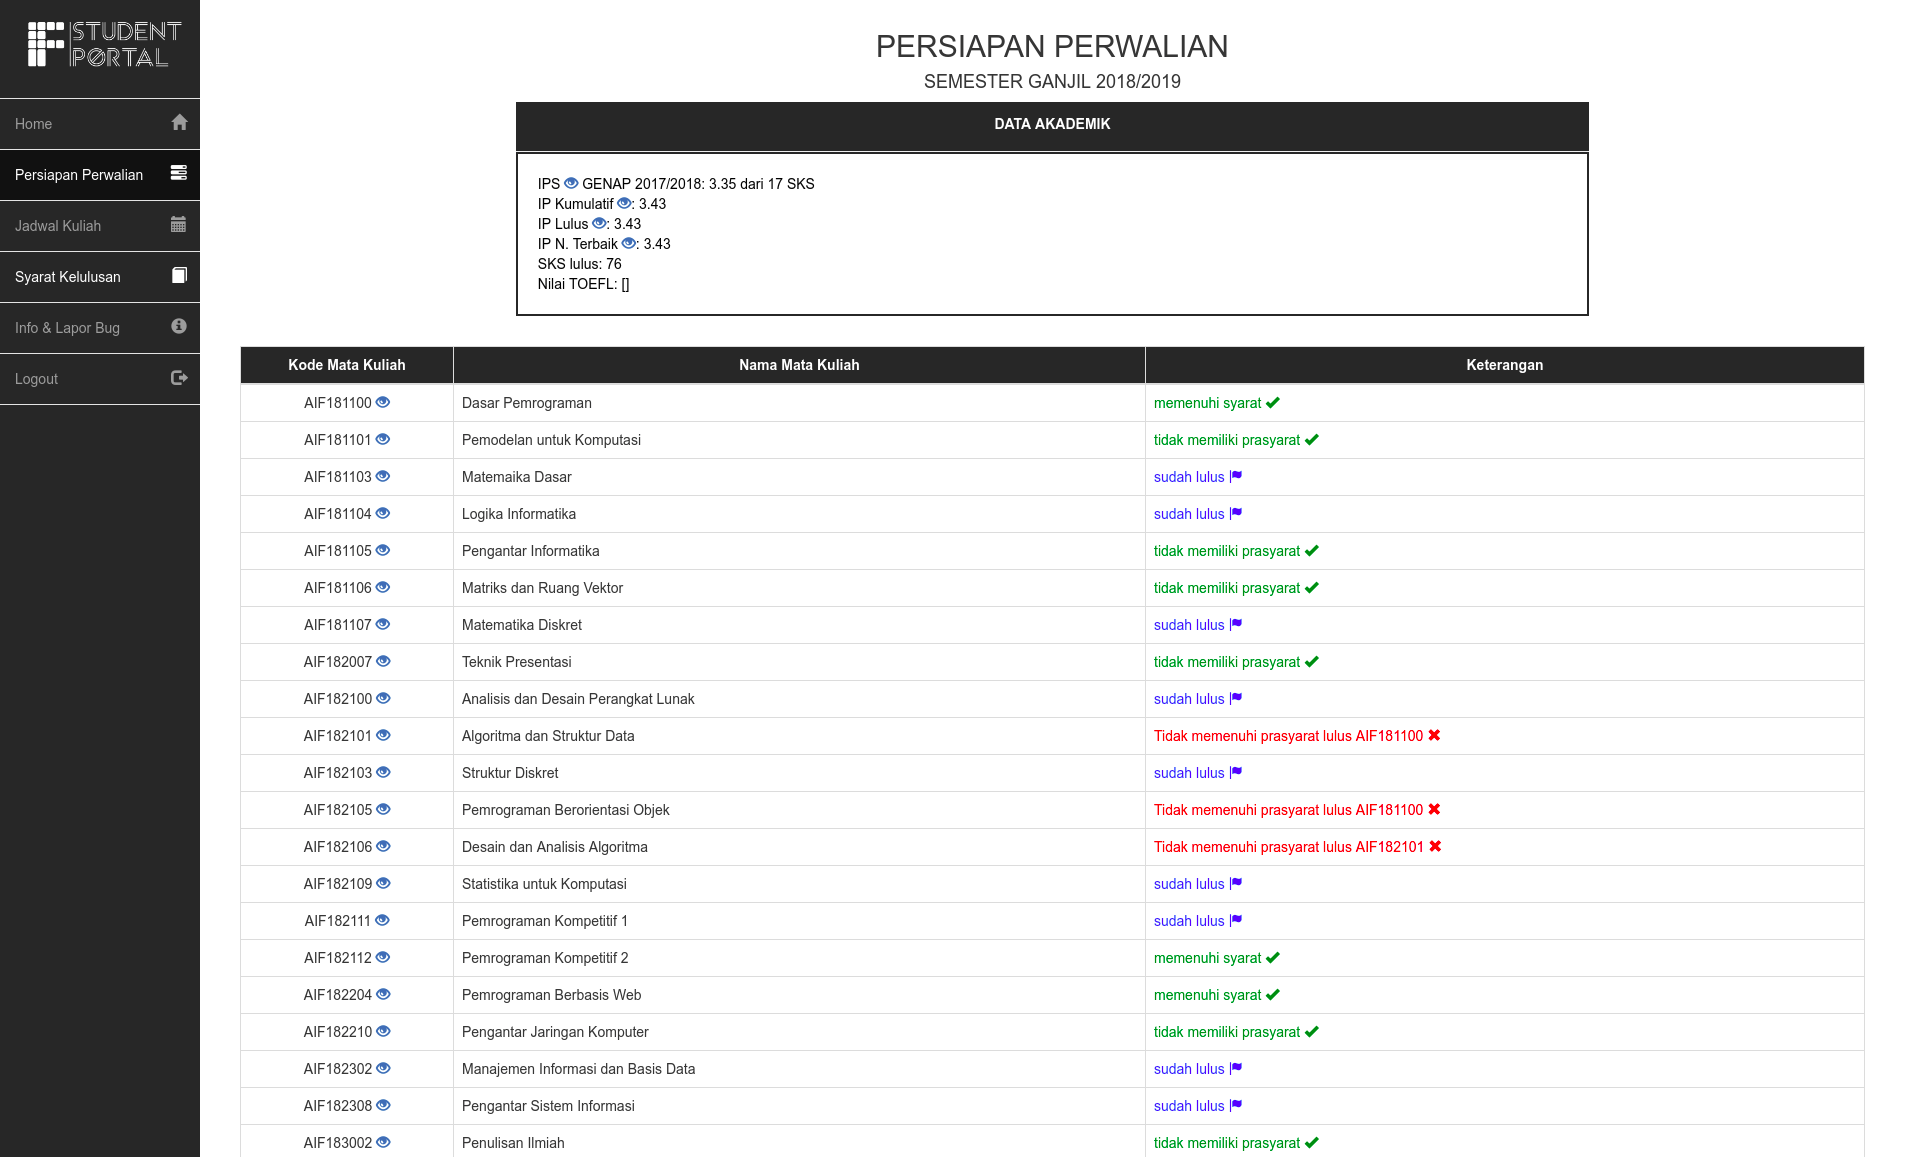
\includegraphics[scale=0.25]{Gambar/HasilPengujian/2016_1_persiapan_perwalian_ifstudentportal}
			\caption{Halaman Persiapan Perwalian (IFStudentPortal) - Gunawan Christianto}
			\label{fig:2016_1_persiapan_perwalian_ifstudentportal}
		\end{figure}
		\begin{figure}[H]
			\centering
			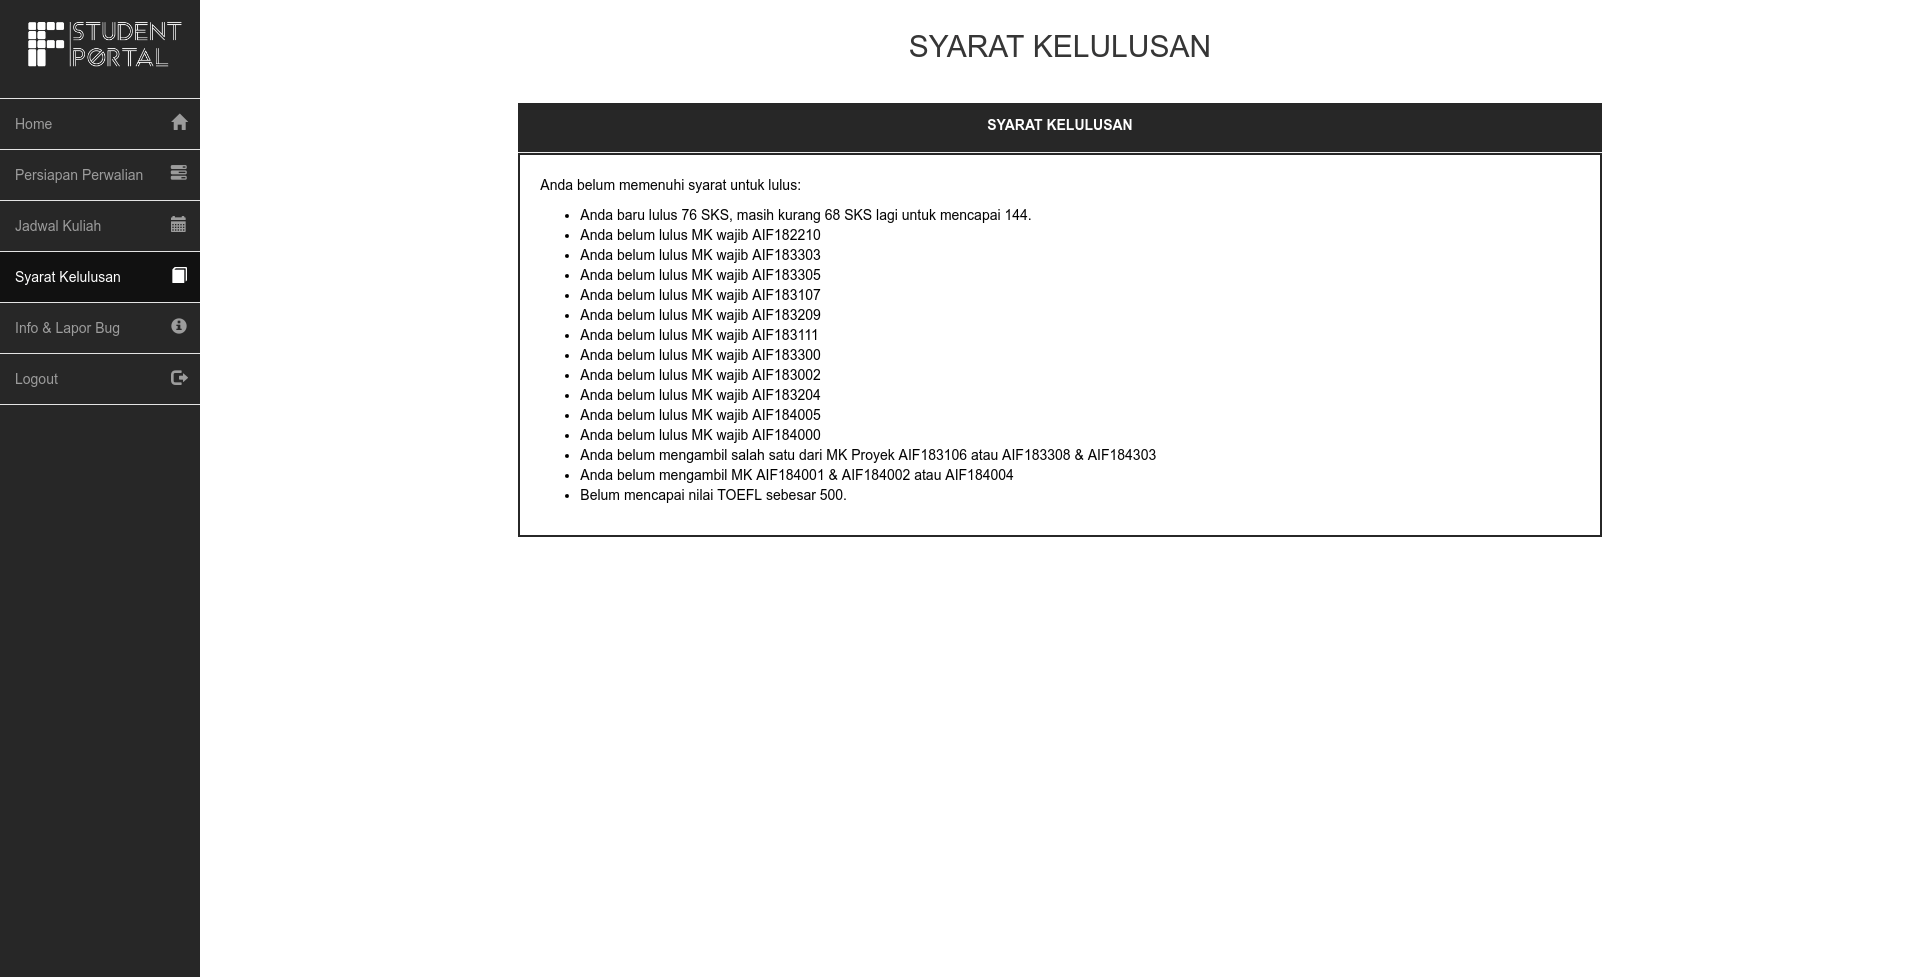
\includegraphics[scale=0.25]{Gambar/HasilPengujian/2016_1_syarat_kelulusan_ifstudentportal}
			\caption{Halaman Syarat Kelulusan (IFStudentPortal) - Gunawan Christianto}
			\label{fig:2016_1_syarat_kelulusan_ifstudentportal}
		\end{figure}
		\begin{figure}[H]
			\centering
			\includegraphics[scale=0.25]{Gambar/HasilPengujian/2016_1_nps_studentportal}
			\caption{Halaman Nilai Per Semester (Student Portal) - Gunawan Christianto}
			\label{fig:2016_1_nps_studentportal}
		\end{figure}
		\begin{figure}[H]
			\centering
			\includegraphics[scale=0.35]{Gambar/HasilPengujian/2016_1_rip_studentportal}
			\caption{Halaman Riwayat Indek Prestasi (Student Portal) - Gunawan Christianto}
			\label{fig:2016_1_rip_studentportal}
		\end{figure}
		\begin{figure}[H]
			\centering
			\includegraphics[scale=0.25]{Gambar/HasilPengujian/2016_1_toefl_studentportal}
			\caption{Halaman Nilai TOEFL (Student Portal) - Gunawan Christianto}
			\label{fig:2016_1_toefl_studentportal}
		\end{figure}
		\begin{figure}[H]
			\centering
			\includegraphics[scale=0.25]{Gambar/HasilPengujian/2016_1_jadwal_kuliah_ifstudentportal}
			\caption{Halaman Jadwal Kuliah (IFStudentPortal) - Gunawan Christianto}
			\label{fig:2016_1_jadwal_kuliah_ifstudentportal}
		\end{figure}
		\begin{figure}[H]
			\centering
			\includegraphics[scale=0.25]{Gambar/HasilPengujian/2016_1_jadwal_kuliah_studentportal}
			\caption{Halaman Jadwal Kuliah (Student Portal) - Gunawan Christianto}
			\label{fig:2016_1_jadwal_kuliah_studentportal}
		\end{figure}
		Hasil pengujian eksperimental halaman persiapan perwalian dari IFStudentPortal yang berisi data akademik (IPS, IPK, IP Lulus, IP Nilai Terbaik, sks lulus, dan nilai TOEFL) dan data mata kuliah berserta prasyaratnya dapat dilihat pada Gambar \ref{fig:2016_1_persiapan_perwalian_ifstudentportal}. Gambar \ref{fig:2016_1_rip_studentportal} menunjukkan riwayat IP sedangkan Gambar \ref{fig:2016_1_nps_studentportal} menunjukkan salah satu nilai per semester mahasiswa dan Gambar \ref{fig:2016_1_toefl_studentportal} menunjukkan riwayat nilai TOEFL mahasiswa. Hasil tersebut menunjukkan bahwa halaman persiapan perwalian sudah sesuai dengan data mahasiswa pada Student Portal. Hasil pengujian berikutnya dapat dilihat pada Gambar \ref{fig:2016_1_syarat_kelulusan_ifstudentportal} menujukkan syarat lulus mahasiswa Teknik Informatika UNPAR sedangkan Gambar \ref{fig:2016_1_nps_studentportal} menujukkan salah satu data nilai hasil transisi ke kurikulum 2018. Hasil tersebut menunjukkan bahwa halaman syarat kelulusan telah sesuai dengan hasil yang diharapkan. Hasil pengujian berikutnya dapat dilihat pada Gambar \ref{fig:2016_1_jadwal_kuliah_ifstudentportal} menunjukan jadwal kuliah mahasiswa pada IFStudentPortal. Kemudian jadwal kuliah mahasiswa pada Student Portal dapat dilihat pada Gambar \ref{fig:2016_1_jadwal_kuliah_studentportal}. Hasil tersebut menunjukkan bahwa jadwal kuliah dari IFStudentPortal sudah sesuai dengan jadwal kuliah pada Student Portal.
		\item Joshua Lauwrich Nandy - 2016730072 \\
		\begin{figure}[H]
			\centering
			\includegraphics[scale=0.45]{Gambar/HasilPengujian/2016_2_persiapan_perwalian_ifstudentportal}
			\caption{Halaman Persiapan Perwalian (IFStudentPortal) - Joshua Lauwrich Nandy}
			\label{fig:2016_2_persiapan_perwalian_ifstudentportal}
		\end{figure}
		\begin{figure}[H]
			\centering
			\includegraphics[scale=0.45]{Gambar/HasilPengujian/2016_2_syarat_kelulusan_ifstudentportal}
			\caption{Halaman Syarat Kelulusan (IFStudentPortal) - Joshua Lauwrich Nandy}
			\label{fig:2016_2_syarat_kelulusan_ifstudentportal}
		\end{figure}
		\begin{figure}[H]
			\centering
			\includegraphics[scale=0.45]{Gambar/HasilPengujian/2016_2_nps_studentportal}
			\caption{Halaman Nilai Per Semester (Student Portal) - Joshua Lauwrich Nandy}
			\label{fig:2016_2_nps_studentportal}
		\end{figure}
		\begin{figure}[H]
			\centering
			\includegraphics[scale=0.45]{Gambar/HasilPengujian/2016_2_rip_studentportal}
			\caption{Halaman Riwayat Indek Prestasi (Student Portal) - Joshua Lauwrich Nandy}
			\label{fig:2016_2_rip_studentportal}
		\end{figure}
		\begin{figure}[H]
			\centering
			\includegraphics[scale=0.45]{Gambar/HasilPengujian/2016_2_toefl_studentportal}
			\caption{Halaman Nilai TOEFL (Student Portal) - Joshua Lauwrich Nandy}
			\label{fig:2016_2_toefl_studentportal}
		\end{figure}
		\begin{figure}[H]
			\centering
			\includegraphics[scale=0.45]{Gambar/HasilPengujian/2016_2_jadwal_kuliah_ifstudentportal}
			\caption{Halaman Jadwal Kuliah (IFStudentPortal) - Joshua Lauwrich Nandy}
			\label{fig:2016_2_jadwal_kuliah_ifstudentportal}
		\end{figure}
		\begin{figure}[H]
			\centering
			\includegraphics[scale=0.45]{Gambar/HasilPengujian/2016_2_jadwal_kuliah_studentportal}
			\caption{Halaman Jadwal Kuliah (Student Portal) - Joshua Lauwrich Nandy (1/2)}
			\label{fig:2016_2_jadwal_kuliah_studentportal}
		\end{figure}
		\begin{figure}[H]
			\centering
			\includegraphics[scale=0.45]{Gambar/HasilPengujian/2016_2_jadwal_kuliah_studentportal_2}
			\caption{Halaman Jadwal Kuliah (Student Portal) - Joshua Lauwrich Nandy (2/2)}
			\label{fig:2016_2_jadwal_kuliah_studentportal_2}
		\end{figure}
		Hasil pengujian eksperimental halaman persiapan perwalian dari IFStudentPortal yang berisi data akademik (IPS, IPK, IP Lulus, IP Nilai Terbaik, sks lulus, dan nilai TOEFL) dan data mata kuliah berserta prasyaratnya dapat dilihat pada Gambar \ref{fig:2016_1_persiapan_perwalian_ifstudentportal}. Gambar \ref{fig:2016_2_rip_studentportal} menunjukkan riwayat IP sedangkan Gambar \ref{fig:2016_2_nps_studentportal} menunjukkan salah satu nilai per semester mahasiswa dan Gambar \ref{fig:2016_2_toefl_studentportal} menunjukkan riwayat nilai TOEFL mahasiswa. Hasil tersebut menunjukkan bahwa halaman persiapan perwalian sudah sesuai dengan data mahasiswa pada Student Portal. Hasil pengujian berikutnya dapat dilihat pada Gambar \ref{fig:2016_2_syarat_kelulusan_ifstudentportal} menujukkan syarat lulus mahasiswa Teknik Informatika UNPAR sedangkan Gambar \ref{fig:2016_2_nps_studentportal} menujukkan salah satu data nilai hasil transisi ke kurikulum 2018. Hasil tersebut menunjukkan bahwa halaman syarat kelulusan telah sesuai dengan hasil yang diharapkan. Hasil pengujian berikutnya dapat dilihat pada Gambar \ref{fig:2016_2_jadwal_kuliah_ifstudentportal} menunjukan jadwal kuliah mahasiswa pada IFStudentPortal. Kemudian jadwal kuliah mahasiswa pada Student Portal dapat dilihat pada Gambar \ref{fig:2016_2_jadwal_kuliah_studentportal}. Hasil tersebut menunjukkan bahwa jadwal kuliah dari IFStudentPortal sudah sesuai dengan jadwal kuliah pada Student Portal.
	\end{enumerate}
	Hasil pengujian eksperimental dari kedua mahasiswa angkatan 2016 sesuai dengan hasil yang diharapkan.
	\item Angkatan 2017 \\
	Untuk angkatan 2017 pengujian dilakukan kepada dua orang mahasiswa, yaitu:
	\begin{enumerate}
		\item Yohan Kurnia Wijaya - 2017730020
		\begin{figure}[H]
			\centering
			\includegraphics[scale=0.325]{Gambar/HasilPengujian/2017_1_persiapan_perwalian_ifstudentportal}
			\caption{Halaman Persiapan Perwalian (IFStudentPortal) - Yohan Kurnia Wijaya}
			\label{fig:2017_1_persiapan_perwalian_ifstudentportal}
		\end{figure}
		\begin{figure}[H]
			\centering
			\includegraphics[scale=0.325]{Gambar/HasilPengujian/2017_1_syarat_kelulusan_ifstudentportal}
			\caption{Halaman Syarat Kelulusan (IFStudentPortal) - Yohan Kurnia Wijaya}
			\label{fig:2017_1_syarat_kelulusan_ifstudentportal}
		\end{figure}
		\begin{figure}[H]
			\centering
			\includegraphics[scale=0.325]{Gambar/HasilPengujian/2017_1_nps_studentportal}
			\caption{Halaman Nilai Per Semester (Student Portal) - Yohan Kurnia Wijaya}
			\label{fig:2017_1_nps_studentportal}
		\end{figure}
		\begin{figure}[H]
			\centering
			\includegraphics[scale=0.325]{Gambar/HasilPengujian/2017_1_rip_studentportal}
			\caption{Halaman Riwayat Indek Prestasi (Student Portal) - Yohan Kurnia Wijaya}
			\label{fig:2017_1_rip_studentportal}
		\end{figure}
		\begin{figure}[H]
			\centering
			\includegraphics[scale=0.325]{Gambar/HasilPengujian/2017_1_toefl_studentportal}
			\caption{Halaman Nilai TOEFL (Student Portal) - Yohan Kurnia Wijaya}
			\label{fig:2017_1_toefl_studentportal}
		\end{figure}
		\begin{figure}[H]
			\centering
			\includegraphics[scale=0.325]{Gambar/HasilPengujian/2017_1_jadwal_kuliah_ifstudentportal}
			\caption{Halaman Jadwal Kuliah (IFStudentPortal) - Yohan Kurnia Wijaya}
			\label{fig:2017_1_jadwal_kuliah_ifstudentportal}
		\end{figure}
		\begin{figure}[H]
			\centering
			\includegraphics[scale=0.325]{Gambar/HasilPengujian/2017_1_jadwal_kuliah_studentportal}
			\caption{Halaman Jadwal Kuliah (Student Portal) - Yohan Kurnia Wijaya}
			\label{fig:2017_1_jadwal_kuliah_studentportal}
		\end{figure}
		Hasil pengujian eksperimental halaman persiapan perwalian dari IFStudentPortal yang berisi data akademik (IPS, IPK, IP Lulus, IP Nilai Terbaik, sks lulus, dan nilai TOEFL) dan data mata kuliah berserta prasyaratnya dapat dilihat pada Gambar \ref{fig:2017_1_persiapan_perwalian_ifstudentportal}. Gambar \ref{fig:2017_1_rip_studentportal} menunjukkan riwayat IP sedangkan Gambar \ref{fig:2017_1_nps_studentportal} menunjukkan salah satu nilai per semester mahasiswa dan Gambar \ref{fig:2017_1_toefl_studentportal} menunjukkan riwayat nilai TOEFL mahasiswa. Hasil tersebut menunjukkan bahwa halaman persiapan perwalian sudah sesuai dengan data mahasiswa pada Student Portal. Hasil pengujian berikutnya dapat dilihat pada Gambar \ref{fig:2017_1_syarat_kelulusan_ifstudentportal} menujukkan syarat lulus mahasiswa Teknik Informatika UNPAR sedangkan Gambar \ref{fig:2017_1_nps_studentportal} menujukkan salah satu data nilai hasil transisi ke kurikulum 2018. Hasil tersebut menunjukkan bahwa halaman syarat kelulusan telah sesuai dengan hasil yang diharapkan. Hasil pengujian berikutnya dapat dilihat pada Gambar \ref{fig:2017_1_jadwal_kuliah_ifstudentportal} menunjukan jadwal kuliah mahasiswa pada IFStudentPortal. Kemudian jadwal kuliah mahasiswa pada Student Portal dapat dilihat pada Gambar \ref{fig:2017_1_jadwal_kuliah_studentportal}. Hasil tersebut menunjukkan bahwa jadwal kuliah dari IFStudentPortal sudah sesuai dengan jadwal kuliah pada Student Portal.
		\item Henrico Leodra - 2017730038
		\begin{figure}[H]
			\centering
			\includegraphics[scale=0.325]{Gambar/HasilPengujian/2017_2_persiapan_perwalian_ifstudentportal}
			\caption{Halaman Persiapan Perwalian (IFStudentPortal) - Henrico Leodra}
			\label{fig:2017_2_persiapan_perwalian_ifstudentportal}
		\end{figure}
		\begin{figure}[H]
			\centering
			\includegraphics[scale=0.325]{Gambar/HasilPengujian/2017_2_syarat_kelulusan_ifstudentportal}
			\caption{Halaman Syarat Kelulusan (IFStudentPortal) - Henrico Leodra}
			\label{fig:2017_2_syarat_kelulusan_ifstudentportal}
		\end{figure}
		\begin{figure}[H]
			\centering
			\includegraphics[scale=0.325]{Gambar/HasilPengujian/2017_2_nps_studentportal}
			\caption{Halaman Nilai Per Semester (Student Portal) - Henrico Leodra}
			\label{fig:2017_2_nps_studentportal}
		\end{figure}
		\begin{figure}[H]
			\centering
			\includegraphics[scale=0.325]{Gambar/HasilPengujian/2017_2_rip_studentportal}
			\caption{Halaman Riwayat Indek Prestasi (Student Portal) - Henrico Leodra}
			\label{fig:2017_2_rip_studentportal}
		\end{figure}
		\begin{figure}[H]
			\centering
			\includegraphics[scale=0.325]{Gambar/HasilPengujian/2017_2_toefl_studentportal}
			\caption{Halaman Nilai TOEFL (Student Portal) - Henrico Leodra}
			\label{fig:2017_2_toefl_studentportal}
		\end{figure}
		\begin{figure}[H]
			\centering
			\includegraphics[scale=0.325]{Gambar/HasilPengujian/2017_2_jadwal_kuliah_ifstudentportal}
			\caption{Halaman Jadwal Kuliah (IFStudentPortal) - Henrico Leodra}
			\label{fig:2017_2_jadwal_kuliah_ifstudentportal}
		\end{figure}
		\begin{figure}[H]
			\centering
			\includegraphics[scale=0.325]{Gambar/HasilPengujian/2017_2_jadwal_kuliah_studentportal}
			\caption{Halaman Jadwal Kuliah (Student Portal) - Henrico Leodra}
			\label{fig:2017_2_jadwal_kuliah_studentportal}
		\end{figure}
		Hasil pengujian eksperimental halaman persiapan perwalian dari IFStudentPortal yang berisi data akademik (IPS, IPK, IP Lulus, IP Nilai Terbaik, sks lulus, dan nilai TOEFL) dan data mata kuliah berserta prasyaratnya dapat dilihat pada Gambar \ref{fig:2017_2_persiapan_perwalian_ifstudentportal}. Gambar \ref{fig:2017_2_rip_studentportal} menunjukkan riwayat IP sedangkan Gambar \ref{fig:2017_2_nps_studentportal} menunjukkan salah satu nilai per semester mahasiswa dan Gambar \ref{fig:2017_2_toefl_studentportal} menunjukkan riwayat nilai TOEFL mahasiswa. Hasil tersebut menunjukkan bahwa halaman persiapan perwalian sudah sesuai dengan data mahasiswa pada Student Portal. Hasil pengujian berikutnya dapat dilihat pada Gambar \ref{fig:2017_2_syarat_kelulusan_ifstudentportal} menujukkan syarat lulus mahasiswa Teknik Informatika UNPAR sedangkan Gambar \ref{fig:2017_2_nps_studentportal} menujukkan salah satu data nilai hasil transisi ke kurikulum 2018. Hasil tersebut menunjukkan bahwa halaman syarat kelulusan telah sesuai dengan hasil yang diharapkan. Hasil pengujian berikutnya dapat dilihat pada Gambar \ref{fig:2017_2_jadwal_kuliah_ifstudentportal} menunjukan jadwal kuliah mahasiswa pada IFStudentPortal. Kemudian jadwal kuliah mahasiswa pada Student Portal dapat dilihat pada Gambar \ref{fig:2017_2_jadwal_kuliah_studentportal}. Hasil tersebut menunjukkan bahwa jadwal kuliah dari IFStudentPortal sudah sesuai dengan jadwal kuliah pada Student Portal.
	\end{enumerate}
	Hasil pengujian eksperimental dari kedua mahasiswa angkatan 2017 sesuai dengan hasil yang diharapkan.
	\item Angkatan 2018 \\
	Untuk angkatan 2018 dilakukan kepada satu orang mahasiswa, yaitu:
	\begin{itemize}
		\item Juan Antonius - 6181801059 \\
		\begin{figure}[H]
			\centering
			\includegraphics[scale=0.3]{Gambar/2018_1_error}
			\caption{\textit{Login error} mahasiswa Juan Antonius}
			\label{fig:2018_1_error}
		\end{figure}
		Pengujian eksperimental dilakukan kepada mahasiswa bernama Juan Antonius. Disini Juan tidak dapat \textit{login} ke IFStudentPortal dan IFStudentPortal mengeluarkan pesan \textit{error} yaitu ``bukan mahasiswa teknik informatika'' (Gambar \ref{fig:2018_1_error}). Ternyata pada angkatan 2018 terdapat perbedaan format NPM mahasiswa, sehingga pengujian eksperimental tidak dapat dilakukan karena aplikasi tidak menangani perbedaan format NPM mahasiswa.
		\item Angkatan yang sudah lulus \\
		\begin{figure}[H]
			\centering
			\includegraphics[scale=0.45]{Gambar/HasilPengujian/2012_1}
			\caption{\textit{Error Login} IFStudentPortal}
			\label{fig:2012_1}
		\end{figure}
		\begin{figure}[H]
			\centering
			\includegraphics[scale=0.45]{Gambar/HasilPengujian/2012_2}
			\caption{\textit{Error Login} Student Portal UNPAR}
			\label{fig:2012_2}
		\end{figure}
		Pengujian eksperimental ini dilakukan untuk mengetahui apakah yang mahasiswa yang telah lulus dapat mengakses IFStudentPortal. Pengujian dilakukan pada mahasiswa Tommy Adhitya The (2012730031). Hasil yang diperoleh dari pengujian ini bahwa mahasiswa Tommy tidak dapat mengakses IFStudentPortal (Gambar \ref{fig:2012_1}) karena mahasiswa Tommy sudah tidak dapat mengakses Student Portal yang diperlihatkan pada Gambar \ref{fig:2012_2}.
	\end{itemize}
\end{itemize}